\documentclass[oneside]{book}

\usepackage{style}

% uthsav: adding to write code inline
\newcommand{\codeblock}{\textcolor{blue}}

\newif\ifdraft\drafttrue      % Uncomment to turn on comments
%\newif\ifdraft\draftfalse   % Uncomment to turn off comments

\begin{document}

\frontmatter
	\input{titlepage}
	% \input{copyright}%
	\subsection*{Authors}

TK.

\vspace{5em}

\subsection*{Acknowledgements}

TK.%
	% \input{editor}%
	\input{tableofcontents}
	% \listoffigures
	% \listoftables
	% \lstlistoflistings


\mainmatter
	\chapter{Introduction}

\section{Overview of course}

Knowing just a little bit of computer science can get you started right away in
writing code for real-world applications. In this course, you will learn about
the fascinating subject of computer science. You will develop algorithmic
thinking skills that will imporove day-to-day critical thinking and
problem-solving. Perhaps most importantly, you will learn to code, which will
not only open up new job opportunities but also make you more effective in most
areas of business.

\afm{Is this still true?} In the first semester, the first two classes of each
week focus on computer science theory and special topics. The final day of each
week will be a lab day, where we actually start practicing coding skills.

In the second semester, we will focus more on practical coding, with a single day a week for theory and 2 lab periods per week for coding. 

Broadly, we will cover the following topics:
\begin{itemize}
    \item How modern computers work
    	\begin{itemize}
       		\item Hardware
       		\item Software
       		\item Computer networks and information systems
    	\end{itemize}
    \item Algorithms for quickly solving complex problems
    	\begin{itemize}
       		\item Searching
       		\item Sorting
    	\end{itemize}
    \item Data structures 
    	\begin{itemize}
       		\item Arrays
       		\item ArrayLists
    	\end{itemize}
    \item Applications of Computer science
    	\begin{itemize}
       		\item Basic coding in Java
       		\item How to use productivity software
    	\end{itemize}
    \end{itemize}
    
\begin{figure}
  \centering
    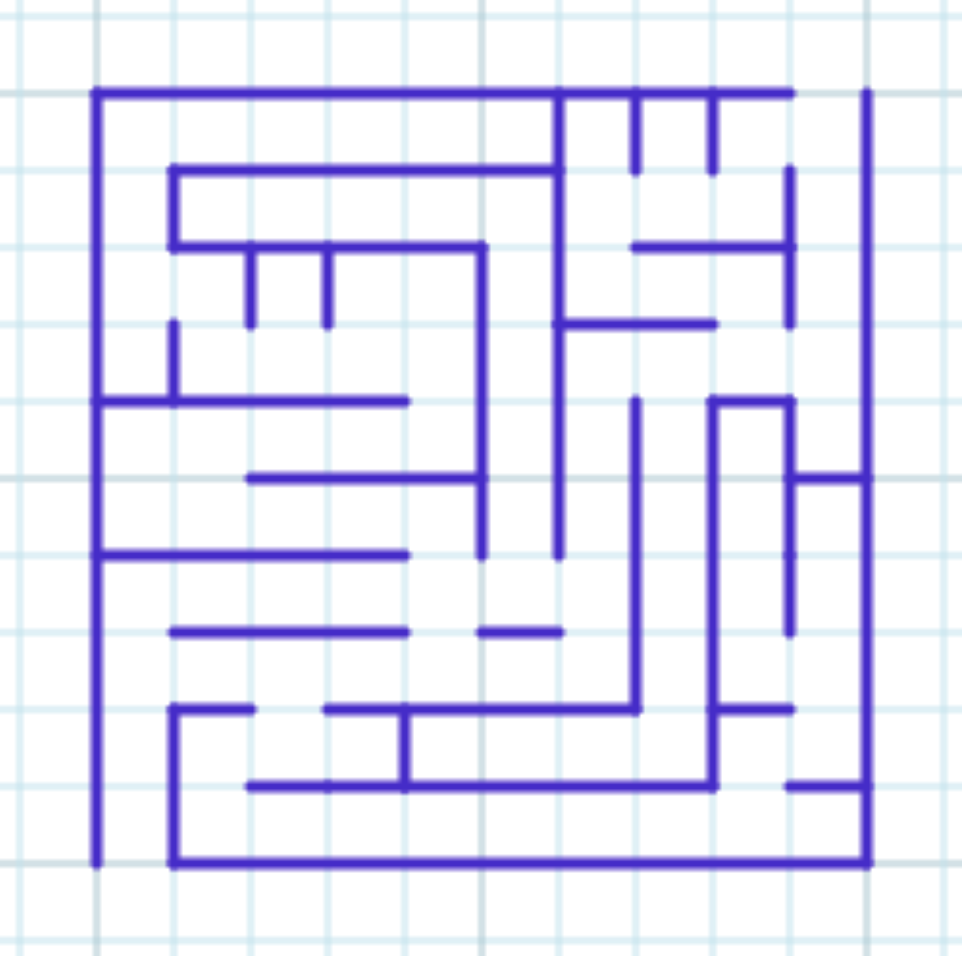
\includegraphics[scale=.4]{graph-paper.png}
    \caption{An example maze. The input is in the lower left, the output is in
      the upper right. Each set of 4 squares counts as one square the robot can
      move into.}
    \label{fig:graph-paper}
\end{figure}

\begin{exercise}
  Get a piece of graph paper, and build a maze on it. Your maze should have one
  input, and one output. An example maze is shown on
  Figure~\ref{fig:graph-paper}.

  Next, get another student's maze. You are programming a robot that can solve
  this maze. These robots can take a sequence of commands, where each command is
  ``Turn Left [number]'' (TL[n]) and ``Move Forwards [number]'' (MF[n]). Create a sequence of inputs to the robots
  that would solve that maze.  For example, the following robot goes to the top
  left corner of the provided maze: MF[2], TL[3], MF[2],
  TL[1], MF[1], TL[1], MF[2], TL[3], MF[7].

  What types of commands could have made this easier? Could your robot solve
  arbitrary mazes? What types of commands would be helpful for making your robot
  solve any maze?
\end{exercise}

\section{Brief history of computer science}

Timeline:\footnote{https://www.worldsciencefestival.com/infographics/a\_history\_of\_computer\_science/}
\begin{itemize}
\item Invention of the abacus (2700-2300 BC, Sumerians)
\item Design of first modern-style computer (Charles Babbage, 1837)
\item Design of first computer algorithm (Ada Lovelace, 1843)
\item Invention of first electronic digital computer (Konrad Zuse, 1941)
\item Invention of the transistor (Bell labs, 1947)
\item Invention of the first computer network (early Internet) (DARPA, 1968)
\item Invention of the World Wide Web (Sir Tim Berners-Lee, 1990)
\end{itemize}

\begin{figure}
	\centering
	\includegraphics[width=0.85\textwidth]{images/z1.jpg}
	\caption{Construction of Konrad Zuse's Z1, the first modern computer, in his
    parents' apartment.
    https://history-computer.com/ModernComputer/Relays/Zuse.html}
	\label{fig:z1}
\end{figure}

\section{Components of a computer}

There are 4 primary components of a computer:

\begin{itemize}
	\item Hardware
	\item Software
	\item Data
	\item User
\end{itemize}

\subsection{Hardware}

Computer hardware consists of physical, electronic devices. These are the parts you actually can see and touch. Some examples include

\begin{itemize}
	\item Central processing unit (CPU)
	\item Monitor
	\item CD drive
	\item Keyboard
	\item Computer data storage
	\item Graphic card
	\item Sound card
	\item Speakers
	\item Motherboard
\end{itemize}

\begin{figure}
	\centering
	\includegraphics[width=0.85\textwidth]{images/hardware.png}
	\caption{Examples of hardware components of a personal computer. https://www5.cob.ilstu.edu/dsmath1/tag/computer-hardware/}
	\label{fig:hardware}
\end{figure}

We will discuss these components in more detail in lecture 3.

\subsection{Software}

Software (otherwise known as \textit{programs}, \textit{applications}, or \textit{apps}) are organized sets of instructions for controlling the computer.

There are two main classes of software:

\begin{itemize}
	\item Applications software: programs allowing the human to interact directly with the computer
	\item Systems software: programs the computer uses to control itself
\end{itemize}

Some more familiar applications software include

\begin{itemize}
	\item Microsoft Word: allows the user to edit text files
	\item Internet Explorer: connects the user to the world wide web
	\item iTunes: organizes and plays music files
\end{itemize}

While applications software allows the user to interact with the computer, systems software keeps the computer running. The operating system (OS) is the most common example of systems software, and it schedules tasks and manages storage of data.

We will dive deeper into the details of both applications and systems software in lecture 4.

\subsection{Data}
Data is fundamentally information of any kind. One key benefit of computers is their ability to reliably store massive quantities of data for a long time. Another is the speed with which they can do calculations on data once they receive instructions from a human user.

While humans can understand data with a wide variety of perceptions (taste,
smell, hearing, touch, sight), computers read and write everything internally as
\textit{bits}, sequences of 0s and 1s.

Computers have software and hardware which allow them to convert their internal 0s and 1s into text, numerals, and images displayed on the monitor; and sounds which can be played through the speaker.

Similarly, computers have hardware and software that convert information from
the real world into bits: a microphone converts sound, a camera converts pictures, and a text editor converts character symbols.

\subsection{Users}
Of course, there would be no data and no meaningful calculations without the human user. Computers are ultimately tools for making humans more powerful.

As we will see in the next section, however, different types of computers have different roles for the user.


\section{Types of computers}

\subsection{Supercomputers}
These are the most powerful computers out there. The are used for problems that take along time to calculate. They are rare because of their size and expense, and therefore primarily used by big organizations like universities, corporations, and the government.

The user of a supercomputer typically gives the computer a list of instructions, and allows the supercomputer to run on its own over the course of hours or days to complete its task.

\begin{figure}
	\centering
	\includegraphics[width=0.85\textwidth]{images/supercomputer.jpg}
	\caption{Summit, a world-class supercomputing cluster at Oak Ridge National Laboratory in Tennessee. https://insidehpc.com/2018/11/new-top500-list-lead-doe-supercomputers/}
	\label{fig:supercomputer}
\end{figure}

\subsection{Mainframe computers}
Although not as powerful as supercomputers, mainframe computers can handle more data and run much faster than a typical personal computer. Often, they are given instructions only periodically by computer programmers, and then run on their own for months at a time to store and process incoming data. For example, census number-crunching, consumer statistics, and transactions processing all use mainframe computers

\subsection{Personal computers}
These are the familiar computers we use to interact with applications every day. Full-size desktop computers and laptop computers are examples

\subsection{Embedded computers}
In the modern ``digital'' age, nearly all devices we use have computers embedded within them. From cars to washing machines to watches to heating systems, most everyday appliances have a computer within them that allows them to function.

\subsection{Mobile computers}
In the past 2 decades, mobile devices have exploded onto the scene, and smartphones have essentially become as capable as standalone personal computers for many tasks.

\section{Why computers are useful}

Computers help us in most tasks in the modern age. We can use them, for example, to:

\begin{itemize}
	\item Write a letter.
	\item Do our taxes.
	\item Play video games.
	\item Watch videos.
	\item Surf the internet.
	\item Keep in touch with friends.
	\item Date.
	\item Order food.
	\item Control robots and self-driving cars.
\end{itemize}

\begin{exercise}
What are some other tasks a computer can accomplish?
\end{exercise}

This is why the job market for computer scientists continues to expand, and why computer skills are more and more necessary even in non-computational jobs.

According to a Stackoverflow survey from 2018,\footnote{https://insights.stackoverflow.com/survey/2018/} 9\% of professional coders on the online developer community have only been coding for 0-2 years. This demonstrates two things:

\begin{enumerate}
	\item The job market for people with coding skills is continually expanding
	\item It doesn't take much to become a coder
\end{enumerate}

Some examples of careers in computer science include

\begin{itemize}
\item IT management / consulting
\item Game developer
\item Web developer
\item UI/UX designer
\item Data analyst
\item Database manager
\end{itemize}

\begin{exercise}
  Think about building a simple video game. What are the hardware, software,
  data needed for this game? What would be the minimal hardware, and what
  hardware would you need to add features like voice chat or online play. What
  types of computers would best run this game? Why?

  Do the same for a text editor.
\end{exercise}


\referencessection

Computer Science: An Interdisciplinary Approach, Robert Sedgewick and Kevin Wayne.

University of Wisconsin-Madison CS 202 Lectures, Andrea Arpaci-Dusseau.\\http://pages.cs.wisc.edu/~dusseau/Classes/CS202-F11/

	\pagebreak
        \chapter{Hello World}

It is now time for us to start practicing coding skills.
In this course, we will be focusing on learning how to program
in Java, which is just one of many programming languages.
While each programming languages has its own quirks and features
specific to it, many of the concepts you will learn in this
class will exist not only in Java but also in other languages.

We will now write our first program in Java called ``Hello World.''
We will use DrJava to help us write, compile, and run this program.

\section{Starting DrJava}
TODO: how to start DrJava on laptop that students are given
TODO: add screenshot of DrJava when just opened and label parts

On the left-hand side of the window, there is a list of currently-open files. When you first start up DrJava, the only thing there should say ``(Untitled)''.
The main part of the window is where you will write code. There should be numbers along the left-hand side to make it easy for you to see which line you are writing code on. The bottom part of the window is where we can interact with the program, for example by seeing the output of compiling the program or by seeing the output of running the program.

\section{Writing Hello World}

In the main part of the window, type the following code:
\begin{code}
class HelloWorld {
    
    public static void main(String[] args) {
        System.out.println("Hello World!");
    }
    
}
\end{code}

We will learn more about what the different parts of this program do later on, but here is a brief explanation for now:
\begin{enumerate}
\item In line 1, \ic{class HelloWorld} makes a new \emph{class} called \ic{HelloWorld}. In Java, all code must be enclosed in a class. The class contains all the code between the open curly brace \ic{\{} on line 1 and the close curly brace \ic{\}} on line 7.
\item Line 3 makes a new method called \ic{main}. We will learn later what
\ic{public static void} and \ic{String[] args} mean. For now, all you
need to know is that every Java program needs a \ic{main} method and starts
by executing the code within the \ic{main} method. Our \ic{main} method
contains all the code between the open curly brace \ic{\{} on line 3 and the
close curly brace \ic{\}} on line 5.
\item Line 4 is a print statement. \ic{System.out.println} will print out
whatever is specified between the open parenthesis \ic{(} and close
parenthesis\ic{)} that follows immediately after.
\ic{System.out.println} will begin a new line after printing out whatever is specified in the parentheses.
In this case, we
put the \emph{string literal} \ic{"Hello World!"} in between these parentheses.
String literals refer to text between quotation marks.
\end{enumerate}


\section{Saving and Compiling in DrJava}

In the upper part of the window, you should see a toolbar with many buttons.
You can now click the ``Save'' button.
Because the class name is \ic{HelloWorld}, the name of your file will be
\ic{HelloWorld.java}. The \ic{.java} file extension is used for
\emph{source code}, which in this case is human-readable code written in Java.

Clicking the ``Compile'' button will first save your file (if it hasn't already been saved) and then \emph{compile} it. Compiling converts your human-readable
source code into code that is easier for the computer to read.
In the case of Java, this will generate a \ic{.class} file. The
\ic{HelloWorld.class} file contains the compiled code.
After clicking ``Compile,'' the bottom part of the window should say
\ic{Compilation completed.} If there are problems with your program, it may not be able to be compiled. In such a case, this bottom part of the window will instead indicate that there was an issue with compilation.
We can try seeing how this might look now.

Try deleting the final curly brace \ic{\}} from the program and hit ``Compile.''The bottom window should now indicate that something has gone wrong.
The message \ic{Error: reached end of file while parsing} arises because
the end of the file was reached without finding the final curly brace.
Add the curly brace back in and hit ``Compile'' again to recompile the program.
Note that in the bottom part of the window, the ``Compiler Output'' tab is selected. This tab is where you can view any messages from compilation.

Let's see another example of a compilation error. Try deleting the semicolon \ic{;} from the program and hit ``Compile.''
The message \ic{Error: ';' expected} arises because the curly brace on line 5 was reached without the semicolon being
encountered. In Java, every statement must end in a semicolon. In this case, the print statement on line 4 must
end in a semicolon. Add the semicolon back in and recompile the program. Compilation should succeed.

\section{Running Code with DrJava}
Now that the program has been written and compiled, it is now time to run it.
We can use DrJava to run a compiled program by clicking the ``Run'' button in the toolbar. In the bottom part of the window, you should see something like the following:
\begin{code}
> run HelloWorld
Hello World!
>
\end{code}
The \ic{run HelloWorld} part indicates that the program \ic{HelloWorld} should be run, and the next line is the output of the program.
Note that in the bottom part of the window, the ``Interactions'' tab is now
selected. This tab allows you to interact with your program. Clicking
the ``Run'' button is equivalent to clicking the ``Interactions'' tab, typing
\ic{run HelloWorld}, and then hitting enter/return key on your keyboard.

If you would like, you can type \ic{run HelloWorld} after the final \ic{>} and
type the enter/return key to run your program again.

\section{Making Changes}
Now we've successfully written, compiled, and ran our first Java program.
As an exercise, let's make our ``Hello World!'' more enthusiastic.
Change the \ic{Hello World!} in line 4 to \ic{Hello World!!}.
You can compile and rerun your program to see the results. In general,
you can make changes to your program, recompile it, and run it again
to see the results of your changes.

Let's make some other changes.
Try adding \ic{ //print hello} to the end of line 4, so that your line 4 now looks like this:
\begin{code}
        System.out.println("Hello World!!"); // print hello
\end{code}
Try compiling and running the program. The behavior should remain unchanged from the previous time you ran the program.
Two forward slashes \ic{//} denote the beginning of an \emph{inline comment} and have the effect of
turning the rest of the line into a \emph{comment}. Comments are ignored by the compiler and do not have any effect on
the program's behavior. They are
useful for adding explanations or providing information to people that are reading the code. In this case,
the comment \ic{print hello} can be viewed as explaining the purpose of the code on that line.

Now try adding \ic{//} to the beginning of line 4, so that it looks as follows:
\begin{code}
//        System.out.println("Hello World!!"); //print hello
\end{code}
Try compiling and running the program now. You should find that there is now no output. The two forward slashes that you added turned the whole line into a comment. As far as the compiler is concerned, your program is the same
as if the entire line 4 did not exist.

Uncomment line 4 by deleting the forward slashes you added at the beginning of it.
Now add the following lines after line 4:
\begin{code}
System.out.println("Hello!"); // print hello again
System.out.println("Goodbye World!"); // say goodbye
\end{code}
Your code now has \emph{multiple statements}. In particular, you now have three. The first one on line 4 will print
\ic{Hello World!!}, the second one will print \ic{Hello!}, and the third will print \ic{Goodbye World!}.
Note that each of these statements is followed by a semicolon.
Deleting any one of these semicolons will result in a compilation error (give it a try!).
Your code should now look as follows:
\begin{code}
class HelloWorld {
    
    public static void main(String[] args) {
        System.out.println("Hello World!!"); //print hello
        System.out.println("Hello!"); // print hello again
        System.out.println("Goodbye World!"); // say goodbye
    }
    
}
\end{code}
Try compiling it and running it. The output should look as follows:
\begin{code}
Hello World!!
Hello!
Goodbye World!
\end{code}

Let's add some description of what we're doing by adding a \emph{block comment}.
A block comment begins with \ic{/*} and is ended whenever \ic{*/} is encountered.
It may (but does not necessarily need to) span multiple lines.
Right before the main method, add a block comment to get the following:
\begin{code}
class HelloWorld {

    /* Main method to print out the following:
         Hello World!!
         Hello!
         Goodbye World!
    */
    public static void main(String[] args) {
        System.out.println("Hello World!!"); //print hello
        System.out.println("Hello!"); // print hello again
        System.out.println("Goodbye World!"); // say goodbye
    }

}
\end{code}
If you compile and run the program now, it should have the same behavior as before, since whatever occurs
inside comments does not affect the program's behavior.

Inline comments can be nested inside block comments, so for example, the following program
will compile without issue:
\begin{code}
class HelloWorld {

    /* Main method to print out the following:
         Hello World!!
         Hello!
         Goodbye World!
    */
    public static void main(String[] args) {
        /*
        System.out.println("Hello World!!"); //print hello
        System.out.println("Hello!"); // print hello again
        System.out.println("Goodbye World!"); // say goodbye
        */
    }

}
\end{code}
Note that since we have commented out all the code in the main method,
this program is actually the same as the following program that we considered earlier:
\begin{code}
class HelloWorld {

    public static void main(String[] args) {
//        System.out.println("Hello World!!"); //print hello
    }

}
\end{code}

Let's now consider the following program that has two print statements and no comments:
\begin{code}
class HelloWorld {

    public static void main(String[] args) {
        System.out.println("Hello!");
        System.out.println("Goodbye!");
    }

}
\end{code}
Try compiling and running the program. Note the output.
What happens when we remove the linebreaks and spaces between each pair of print statements?
Try removing them to get the following:
\begin{code}
class HelloWorld {

    public static void main(String[] args) {
        System.out.println("Hello!");System.out.println("Goodbye!");
    }

}
\end{code}
Now compile and run the program. What happens?
The behavior should still be such that it prints the same output:
\begin{code}
Hello!
Goodbye!
\end{code}
\emph{Whitespace} such as linebreaks and spaces do not have any meaning in Java.
While spaces are necessary to separate things like \ic{class} and \ic{HelloWorld} or \ic{String[]} and \ic{args}
so that Java can distinguish between them, spaces are otherwise unimportant.
Linebreaks have no significance at all in a Java program except to denote when an inline comment
should end.

That being said, whitespace should be used to make your code more legible. Although you can write
all your Java programs on a single line, it is considered very bad style!
For demonstrative purposes, here the original Hello World Java program all on two lines:
\begin{code}
class HelloWorld{public static void main(String[] args)
    {System.out.println("Hello World!");}}
\end{code}
Try compiling and running it. It should print \ic{Hello World!} as its output.
You can get rid of all the spacing after the close parenthesis \ic{)} to get it all on one line--it
just doesn't fit on the page if it's all on one line here!

        \pagebreak
	\chapter{Hardware}

\begin{figure}
	\centering
	\includegraphics[width=0.85\textwidth]{images/computer_system.png}
	\caption{A variety of computer systems: desktops, a laptop, a tablet, and a
    smart phone. \afm{Source for pic.}}
	\label{fig:hardware:computers}
\end{figure}

Today's lecture will focus on \emph{computer systems} \afm{should we change the title
  to systems, this is funky to say the chapter is hardware, and then say we
  focus on systems}, groupings of devices that work together to perform a common
task (or tasks). A user will interact with a computer through a variety of input
and output devices. These devices include keyboards, mice, speakers, microphones, and monitors. A
user's input will be processed, some computations will be performed, and then
the resulting output will be displayed to the user. When most of us think about
computers, we often think of a desktop or laptop computer, equipped with a
keyboard, mouse, and monitor as seen in Figure~\ref{fig:hardware:computers}.
However, many things we interact with daily are computerized, including cell
phones, cars, traffic lights, smart watches, televisions, and manufacturing
lines. Today each of these items have sensors to perceive the real world, use an
embedded computing device to understand the sensory input, and use a combination
of display and mechanical devices to interact with the real world.

\begin{example}
  For intersections across busy roadways, some traffic lights are computerized
  to optimize road traffic. These lights will stay green along the busier of the
  two roads, and use cameras or pressure sensors to detect the presence of cars
  along the less busy of the two roads. When cars arrive, the lights switch,
  allowing the cars on the less busy road to cross.
\end{example}

Today we will introduce three fundamental parts of computer systems:
input and output devices, memory, and the central processing unit (CPU).
These components work together to perform the basic building blocks of
input processing, storage, control, and output. Understanding how the
three parts work together will allow us to create powerful information
processing tools. We will introduce each of these parts in turn.
In Figure~\ref{fig:hardware:overview}, we see how these parts come
together to form a computer system.

\begin{figure}
	\centering
	\includegraphics[width=0.85\textwidth]{images/cs_intro_hardware_overview.png}
	\caption{Interconnected parts of a computer system (keyboard, mouse,
                 monitor, DVD player / burner, speaker, hard drive, CPU).
                 \afm{source for pic}}
	\label{fig:hardware:overview}
\end{figure}

\section{Input and Output Devices}

Input and output (IO) devices allow the computer to interact with users and the world
directly. Without these devices, a computer system would be very boring, always
performing the same computation each time it's used. Even if it did compute a
different value we would be unable to examine the value. A computer needs to be
able to accept input and provide output. The first computers would occupy a
large room in an office building and connect to a terminal (a keyboard and a
text screen) in another room for users to interact with. Thanks to the hard work
of electrical engineers,
computers can now fit in the palm of your hand while being much more powerful.
Likewise, many more types of input and output devices are now available. We
still have the keyboard and monitor, and the mouse was invented for interacting
with graphical displays. Today's phones are more computer than phone, coming
equipped with speakers, microphones, touch screens, cameras, fingerprint
scanners, radio transmitters, and much more. Computers even come embedded in
other devices like cars, traffic lights, X-ray machines, and thermostats to both
control and monitor the devices. As shown in Figure~\ref{fig:hardware:overview},
these devices connect to the rest of the computer through the computer's memory.
This kind of input and output is called memory mapped I/O (input and output).
Creators of input (or output) devices are assigned a section of the computer’s memory to write (for input devices) or read (for output devices) data. For example, a keyboard might write data about each key that is pressed to a given location. The computer will then read the data in that location to communicate with the keyboard. In the case of an output device, the process works in reverse: the computer writes the data in the assigned location, which the output device then reads. The creators of these devices agree on a known format to read and write data.

\begin{example}
  You can think of communication between devices and computer as similar to
  leaving messages for a friend in a locker. Only you and your friend have
  access to this locker, which only holds space for one message. The format you
  agree upon is which language you'll use to speak (e.g. English) and any
  special keywords or phrases. For example, you might agree upon a convention
  like the kind used in radio communication, where one person waits until they
  get an ``Over'' signal before responding with a new message.
\end {example}

The format that devices and computers communicate in are generally very simple
and structured to permit fast and easily understandable communication for
computers and devices.

\begin{example}
A monitor is a graphical display for computers. Let's consider a monitor
connected to a computer that only displays in black and white images
that are 20 x 20 pixels large. The monitor and keyboard agree upon using
the following format to communicate. The format is black and white images
that are 20 x 20 pixels large. Each pixel's value is represented at 0 for
black and 1 for white. Then an image is represented as a 400 = (20 x 20) long
sequence of pixel values. The sequence is ordered left to right, top to bottom.
Now that both the monitor and computer agree upon the communication format, the
computer can write images to the section of memory dedicated to the monitor
and the monitor will read the image and display the image on its screen.
Figure~\ref{fig:hardware:monitor_image} displays an example image, a 
20 x 20 checkerboard with its encoding.

\emph{Note: While this is a simplified example, this is similar to how modern
  graphical displays communicate with computers}.
\end{example}

\begin{figure}
	\centering
        \hspace{0.5cm}
	\begin{minipage}{0.45\textwidth}
		\includegraphics[width=0.90\textwidth]{images/checkered_image.jpg}
	\end{minipage}
        \begin{minipage}{0.45\textwidth}
		\scriptsize
\begin{verbatim}
0 1 0 1 0 1 0 1 0 1 0 1 0 1 0 1 0 1 0 1
1 0 1 0 1 0 1 0 1 0 1 0 1 0 1 0 1 0 1 0
0 1 0 1 0 1 0 1 0 1 0 1 0 1 0 1 0 1 0 1
1 0 1 0 1 0 1 0 1 0 1 0 1 0 1 0 1 0 1 0
0 1 0 1 0 1 0 1 0 1 0 1 0 1 0 1 0 1 0 1
1 0 1 0 1 0 1 0 1 0 1 0 1 0 1 0 1 0 1 0
0 1 0 1 0 1 0 1 0 1 0 1 0 1 0 1 0 1 0 1
1 0 1 0 1 0 1 0 1 0 1 0 1 0 1 0 1 0 1 0
0 1 0 1 0 1 0 1 0 1 0 1 0 1 0 1 0 1 0 1
1 0 1 0 1 0 1 0 1 0 1 0 1 0 1 0 1 0 1 0
0 1 0 1 0 1 0 1 0 1 0 1 0 1 0 1 0 1 0 1
1 0 1 0 1 0 1 0 1 0 1 0 1 0 1 0 1 0 1 0
0 1 0 1 0 1 0 1 0 1 0 1 0 1 0 1 0 1 0 1
1 0 1 0 1 0 1 0 1 0 1 0 1 0 1 0 1 0 1 0
0 1 0 1 0 1 0 1 0 1 0 1 0 1 0 1 0 1 0 1
1 0 1 0 1 0 1 0 1 0 1 0 1 0 1 0 1 0 1 0
0 1 0 1 0 1 0 1 0 1 0 1 0 1 0 1 0 1 0 1
1 0 1 0 1 0 1 0 1 0 1 0 1 0 1 0 1 0 1 0
0 1 0 1 0 1 0 1 0 1 0 1 0 1 0 1 0 1 0 1
1 0 1 0 1 0 1 0 1 0 1 0 1 0 1 0 1 0 1 0
\end{verbatim}
        \end{minipage}
	\caption{An example checkered image and its encoding --- newlines and spaces added for readability.}
	\label{fig:hardware:monitor_image}
\end{figure}

\section{Memory}

With \emph{memory}, computers gain the ability to store and recall data. This is very
similar to physical storage of items. Figure~\ref{fig:hardware:storage} shows
three storage locations --- a storage closet, a garage, and a warehouse. Each of
the three locations make a tradeoff between convenience of location and storage
capacity. The closet can contain a few things and is the same room you need it.
The garage can fit even more things and is only a walk outside (or through) your
home, and the warehouse can fit practically anything you would want to store but
you have to drive to the warehouse to pick-up or store your items. Similarly, a
computer's memory makes the same trade-offs.

There are two major types of memory, \emph{Main Memory} (RAM) and \emph{Secondary Memory},
like hard disks, solid-state drives, tape drives, and more. Main memory is \emph{volatile},
meaning that the contents of the memory is not preserved when a computer is
turned off and back on. On the other hand Secondary Memory is meant to be
\emph{persistent} or \emph{nonvolatile}, and does not go away when the computer is turned off. Main Memory
can be thought of as the ``scratch paper'' the computer uses for computations.
Computers will also use Main Memory as a conduit for communicating between the
CPU and all other parts of the computer. Main memory is closer to a garage
(where you can lose items when you turn off the lights) --- there is enough room
to fit most items you use regularly and is close enough to not worry about the
time it takes to get to the garage.

In most modern computers,
programs are treated as data. The individual instructions that combine
to form a program are stored in memory just as data is. It is the job of the
computer to properly understand if a segment of memory is data or a program.
The computer is able to fetch data from Secondary Memory to Main Memory or
persist data in Main Memory to Secondary Memory when needed. However,
this process of transferring data between Secondary and Main Memory can
cost a lot of time relative to keeping data in Main Memory only.

\begin{figure}
	\centering
	\includegraphics[width=0.85\textwidth]{images/storage.png}
	\caption{Storage closet, garage, and warehouse trading off between
                 capacity and locality. \afm{picture references}}
	\label{fig:hardware:storage}
\end{figure}

\section {Central Processing Unit}

The final part of a computer we will introduce today is the \emph{central processing
unit} (CPU), also known as the \emph{processor} or \emph{main processor}. The CPU is the physical
circuitry of a computer that performs instructions.

The CPU has several key components: the control logic, arithmetic and logic unit (ALU), registers,
program counter, and clock. These components work together to 
fetch, decode, and execute all instructions --- the building blocks of all programs.
Instructions vary between different brands of CPUs, but, in general, they will
include arithmetic, control, read (from memory), and write (to memory) functionalities.

Example~\ref{ex:hardware:instr} shows several instructions
that together would perform \ic{x = x + y}, given \ic{x} is stored in memory
location 16 and \ic{y} at memory location 20. These instructions are quite low
level, and harder for humans to read than the programs we will write in this course.
However, the programs we write will be translated into these instructions to be
easily understood and executed by the CPU.

\begin{example}
\label{ex:hardware:instr}
\begin{verbatim}
load R1 16    -- Load value at memory location 16 into register 1
load R2 20    -- load value at memory location 20 into register 2
add  R1 R2 R1 -- add the value in register 1 to the value in register 2
                 and store in register 1
store R1 16   -- store the value in register 1 to memory location 16
\end{verbatim}
\end{example}

A key component of a CPU is its clock. The clock allows the CPU to progress in time,
triggering the time to progress from time \ic{t} to time \ic{t + 1}. A single time
segment is referred to as a clock cycle. You might have heard about a computer's CPU
speed. For example, your computer may run at 2.4 GHz = 2.4 billion clock cycles per second. This
is determined by how fast the clock transitions from one time step to the next. This
clock drives the progress of the CPU. The time an instruction takes is measured
in instruction cycles. The rate of the CPU's clock is determined by the slowest
operation of the CPU.

In addition to clocks, the CPU contains a group of memory locations called registers.
A single register is capable of holding a single ``word'' of information. A ``word'' is the smallest
unit of data in a computer. The key benefit of registers is the ability for the
CPU to immediately read and write the contents of the register. The value of a register
can be updated each time the computer's clock ``ticks,'' or increments its value by one. 
Most modern CPU's will have between 16 and 64 registers that programs may use.
For comparison, accessing Main memory can take 10s or even 100s of instruction
cycles to access while registers are immediately available to the CPU.

The control unit and program counter will fetch, decode, and output the
controls for the execution of each instruction. The program counter holds the
location of the next instruction to be executed. The next instruction is then
fetched to the CPU. The CPU's control unit then decodes the fetched instruction
and outputs control signals (commands) to main memory and the ALU. The CPU may
read data from memory (e.g. store) and then the ALU will then execute the action
specified by the control unit. Example actions include add, subtract, multiply, compare to 0, etc.
The CPU may then possibly write the output to memory.

In most computers, the CPU and its constituent parts are responsible for all
computing needs of the computer. In some select systems, there will be additional
hardware to perform specialized operations (e.g. graphics processing units for
processing / producing images). It is the CPU's responsibility to control the
computer and coordinate with devices to execute programs. As such, the CPU
has seen a quick evolution to increase its processing power. Electrical
engineers originally focused on making the CPU smaller and smaller and thus
quicker. The evolution follows Moore's Law : every two years the size of a CPU shrinks
in half. Additionally, CPU's were designed with a pipelining architecture: this means
that multiple instructions are executed in quick succession. This is done
by noting that each stage of the five stages --- fetch, load,  decode, execute,
and store --- can be performed independently. Thus, while one instruction is
being executed, the next instruction can be decoded. Figure~\ref{fig:hardware:pipeline}
shows how pipelining is performed by executing the different parts of the pipeline
in parallel for five consecutive instructions.

Due to the decline of Moore's Law in recent years, many CPU designers focus on
increasing processing power by improving parallelism (i.e. being able to execute
multiple instructions at a time). This allows instructions that do not depend
on each other to be executed at the same time. These CPUs are referred to as multi-core,
as they have multiple cores that each have their own set of registers, control unit,
ALU, and program counter but share main memory and a single clock. In this class we will not
teach how to effectively harness parallel programming, but note that this is
an important progress in how hardware has evolved.

\begin{figure}
	\centering
	\includegraphics[width=0.85\textwidth]{images/pipeline.png}
	\caption{Instruction Pipelining. \afm{citation}}
	\label{fig:hardware:pipeline}
\end{figure}


\section {Conclusion}
In this chapter, we covered the three fundamental parts of a computer system:
input and output devices, Main and Secondary Memory, and the CPU. We discussed
their roles, relationships, and basic capabilities. I hope that this will help
you better understand how hardware works at a high level to better improve how
to write programs that will eventually run on these computer systems. In the
next chapter we will begin discussing the concept of Software and how its
similarities and differences to hardware and where the boundary between the two
lies.

\exercisesection

\begin{exercise}
What three parts comprise a computer system?
\end{exercise}

\begin{exercise}
What are examples of common input and output devices?
\end{exercise}

\begin{exercise}
Name an uncommon example of a computer system and explain how it may work.
\end{exercise}

\begin{exercise}
How does memory mapped input and output work?
\end{exercise}

\begin{exercise}
Name four kinds of memory devices.
\end{exercise}

\begin{exercise}
Explain the difference between Main and Secondary Memory.
\end{exercise}

\begin{exercise}
What parts comprise the central processing unit (CPU)?
\end{exercise}

\begin{exercise}
Describe three possible methods to increase the computation power of a CPU.
\end{exercise}

	\pagebreak
	\chapter{Types and Variables}

We have seen a program that can print a simple ``Hello World'' message to the screen. Next we will learn about basic types of data that can be used in a Java program to perform calculations.

In this chapter, we will first learn about different types of data, focusing on five Java data types: \ic{int}, \ic{double}, \ic{boolean}, \ic{char}, and \ic{String}. Then we will learn about arithmetic, comparison, and logical operators over those types. Finally, we will learn about variables.

\section{Data types}
We work with different types of data all of the time: numbers, text, images, true/false or yes/no information, etc. Since we interact with numbers all the time, we can categorize numeric data in two ways: as (1) integers, which are whole numbers, or as (2) floating point numbers, which are numbers with digits after a decimal point or a fractional component.

Imagine the data you would find on a report card. It would probably have a lot of textual data, such as the student's name and their course names. It would probably also have a lot of numeric data, such as their age or their GPA. \ref{table:report_card} lists examples of information one might find on a report card.

\begin{table}[h!]
\centering
\begin{tabular}{ |c|c|c| }
 \hline
 Item & Example & Type of data \\
 \hline
 \hline
 Student name & John Doe & Text \\
 Course name & Honors Physics & Text \\
 Age & 17 & Integer (whole number) \\
 GPA & 3.75 & Floating point number\\
 \hline
\end{tabular}
\caption{Examples of pieces and types of data typically found on a report card.}
\label{table:report_card}
\end{table}

Now imagine an ice cream menu. It might have pictures of different flavors, along with the names of each flavor. It would probably list prices for different sizes and cones. It might also contain yes/no information, such as whether or not a certain flavor is dairy-free. \autoref{table:ice_cream_menu} lists examples of information one might find on such a menu.

\begin{table}[h!]
\centering
\begin{tabular}{ |c|c|c| }
 \hline
 Item & Example & Type of data \\
 \hline
 \hline
 Ice cream flavor & Mint Chocolate Chip & Text \\
 Price & \$3.99 & Floating point number \\
 Dietary information & Dairy-free & Yes/no \\
 \hline
\end{tabular}
\caption{Examples of pieces and types of data typically found on a menu at an ice cream shop.}
\label{table:ice_cream_menu}
\end{table}

\begin{example}
Take a look at the New Jersey driver's license in \autoref{fig:drivers_license}. List examples of different types of data you can find on it. \\

\noindent \emph{Answer}: Text (name, address), integers (date of birth, height, license number), yes/no (organ donor status).
\end{example}

\begin{figure}[h!]
  \centering
  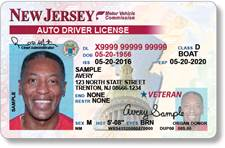
\includegraphics[width=0.5\textwidth]{images/nj_drivers_license}
  \caption{An example of a New Jersey driver's license. TODO: reference \href{https://www.state.nj.us/mvc/images/vetdefig.jpg}{the NJ state website (link here).}}
  \label{fig:drivers_license}
\end{figure}

We are surrounded by different types of data every day. We intuitively understand that different types of data interact in different ways. For example, you can add up the prices of multiple flavors of ice cream, but you cannot divide a student's name by their GPA. The same is true of data types in a Java program.

\begin{definition}
A \emph{data type} is a set of values and a set of operations defined on them.
\end{definition}

In the following sections, we will learn how Java represents different types of data: numeric data, true/false or yes/no data, and textual data. Specifically, we will focus on five types: \ic{int}, \ic{double}, \ic{boolean}, \ic{char}, and \ic{String}.

\subsection{Numeric data}
Representing numbers on a computer requires physical memory. For this reason, Java has six possible types for numeric data: four integer types (\ic{byte}, \ic{short}, \ic{int}, \ic{long}) and two floating point types (\ic{float}, \ic{double}). Some of these types require more memory in order to represent larger numbers, while other types use much less memory and can only represent small numbers. \autoref{table:numeric_types} summarizes this tradeoff between memory storage and numeric range or precision.

\begin{table}[h!]
\centering
\begin{tabular}{ |c|c|p{4.5cm}|p{4.5cm}| }
 \hline
 Type & Storage & Minimum Value & Maximum Value \\
 \hline
 \hline
 \ic{byte} & 8 bits & -128 & 127 \\
 \hline
 \ic{short} & 16 bits & -32,768 & 32,767 \\
 \hline
 \ic{int} & 32 bits & -2,147,483,648 & 2,147,483,647 \\
 \hline
 \ic{long} & 64 bits & -9,223,372,036,854,775,808 & 9,223,372,036,854,775,807 \\
 \hline
 \ic{float} & 32 bits & Approximately -3.4E+38 with 7 significant digits & Approximately 3.4E+38 with 7 significant digits \\
 \hline
 \ic{double} & 64 bits & Approximately -1.7E+308 with 15 significant digits & Approximately 1.7E+308 with 15 significant digits \\
 \hline
\end{tabular}
\caption{Java's six primitive numeric data types along with their memory requirements, range, and precision.}
\label{table:numeric_types}
\end{table}

In this course, we will focus on two of these numeric types: \ic{int} for integers and \ic{double} and floating-point numbers. We use \ic{int}s frequently in Java programs because integers, or whole numbers, show up naturally in everyday life. We also \ic{double}s frequently in Java programs because floating point numbers often show up naturally in scientific applications. A \ic{double} in Java can either be written as a number with a decimal point (e.g. \ic{3.1415} or \ic{4.0}) or using scientific notation (e.g. \ic{6.022e23}). The \ic{e} in this notation is shorthand for ``times 10 to the power of \_\_\_\_''. For example, \ic{6.022e23} is equivalent to $6.022 \times 10^{23}$.

\begin{example}
What are examples of integers in everyday life? \\

\noindent \emph{Answer}: Age (7), number of siblings (2), the result of a dice roll (5), approximate population in New Jersey (8,908,520)
\end{example}

\begin{example}
What are examples of floating point numbers in everyday life? \\

\noindent \emph{Answer}: GPA (4.0), price of a chocolate bar (\$1.99), balance in bank account (\$514.66), average rating out of 5 stars (4.5 out of 5).
\end{example}

\begin{example}
What is the value of \ic{1.23e3}? \\

\noindent \emph{Answer}: It is $1.23 \times 10^3 = 1.23 \times 1000 = 1230$.
\end{example}

\subsection{True/false data}
To represent true/false, yes/no, or on/off data, Java uses \ic{boolean}s. A \ic{boolean} can only be one of two possible values: \ic{true} or \ic{false}. For example, the statement ``The sky is blue right now'' can only either be true or false. If it is daytime, it is most likely true. If it is nighttime or if the sun is currently setting, then it is most likely false. Similarly the statement ``2 plus 2 equals 4'' is clearly true, so we can represent this as a \ic{boolean}. In the same way, we can see that ``3 times 4 is 11'' is false. \ic{boolean}s may seem simple, but we will see soon how to combine them in complex and powerful ways.

\subsection{Textual data}
In general, Java has two main types to represent textual data: a (1) \ic{char} for a single letter or symbol or a (2) \ic{String} for a sequence of multiple letters. A \ic{char} is a single alphanumeric character or symbol, like the ones you can type on your keyboard, that is expressed in Java using single quotes. \ic{'A'}, \ic{'z'}, and \ic{'\$'} are all examples of chars in Java. A \ic{String} is a sequence of characters that is expressed in Java using double quotes. \ic{``Hello World''} is an example of \ic{String}.

\begin{example}
Is \ic{'@'} a valid \ic{char}? \\

\noindent \emph{Answer}: Yes!
\end{example}

\begin{example}
Is \ic{``P''} a valid \ic{char}? \\

\noindent \emph{Answer}: No. A \ic{char} must use single quotes.
\end{example}

\begin{example}
Is \ic{'ABC'} a valid \ic{char}? \\

\noindent \emph{Answer}: No. A \ic{char} must only be a single character.
\end{example}

\begin{example}
What are some examples of \ic{String}s in everyday life? \\

\noindent \emph{Answer}: Text messages, names of friends, email addresses, a poem
\end{example}

\subsection{Summary of five types}
Java has many built-in data types for different types of data: numeric, true/false, and text. In this section, we have focused on five of these types: \ic{int} for integers, \ic{double} for floating point numbers, \ic{boolean} for true/false values, \ic{char} for single characters, and \ic{String} for a sequence of characters. \autoref{table:types_summary} summarizes these five types.

\begin{table}[h!]
\centering
\begin{tabular}{ |c|c|c| }
 \hline
 Type & Description & Examples \\
 \hline
 \hline
 \ic{int} & integers & 5, -100, 1,234,567 \\
 \hline
 \ic{double} & floating point number & 3.75, 6.022e23 \\
 \hline
 \ic{boolean} & true/false value & \ic{true}, \ic{false} \\
 \hline
 \ic{char} & characters & \ic{'A'}, \ic{'\%'}, \ic{'5'} \\
 \hline
 \ic{String} & sequences of characters & \ic{``Hello''}, \ic{``123 Happy St.''} \\
 \hline
\end{tabular}
\caption{A summary of five of Java's built-in types}
\label{table:types_summary}
\end{table}

\section{Operations}
Now that we have learned about data types, we will next learn about the operations we can perform on the the different data types. Specifically, we will learn about arithmetic and comparison operators used with numeric types (e.g. \ic{int}s and \ic{double}s). Then, we will discuss logical operators used with \ic{boolean}s. Finally, we will learn about operations we can perform on \ic{String}s.

\subsection{Arithmetic operators}
Arithmetic operators are generally the ones we are familiar with from elementary school, such as addition (\ic{+}), subtraction (\ic{-}), multiplication (\ic{*}), and division (\ic{/}). For example, \ic{5 + 3} equals \ic{8}, \ic{5.55 - 1.11} equals \ic{4.44}, and \ic{1.5 * 10} equals \ic{15}.

Of these basic arithmetic operators, division is the trickiest because it behaves in a special way with integers. In Java, if you were to divide two integers, you would get an integer as a result. This is intuitive in some cases. For example, \ic{20 / 5} would equal \ic{4}. However, in other cases, we may lose a fractional component. For instance, \ic{21 / 5} also equals \ic{4}. You might think that \ic{21 / 5} should equal \ic{4.2}, but the fractional piece (everything after the decimal point) gets \emph{truncated}, or dropped completely. This is what we call \emph{integer truncation}.

\begin{example}
What is \ic{2 / 2}? What about \ic{3 / 2}? What about \ic{4 / 2}? \\

\noindent \emph{Answer}: \ic{2 / 2} equals {1}. \\
\ic{3 / 2} also equals {1} (after dropping the \ic{.5} from the answer \ic{1.5}). \\
\ic{4 / 2} equals {2}.
\end{example}

Java also has an extra arithmetic operator, called the ``modulo'' operator (or ``mod'' for short), that looks like a percent symbol \ic{\%}. Its purpose is to compute the remainder when dividing two numbers. For example, \ic{13 \% 3}, which we pronounce as ``ten mod three'', is equal to \ic{1} because 13 divided by 3 gives us 4, remainder 1.

\begin{example}
What is \ic{15 \% 10}? What about \ic{6.25 \% 3}? \\

\noindent \emph{Answer}: \ic{15 \% 10} equals \ic{5}. \\
\ic{6.25 \% 3} equals \ic{0.25}.
\end{example}

TODO: Table of arithemic operators \\

In addition to these five arithmetic operators, Java also provides additional mathematical functions that you might find on a basic scientific calculator, such as square root, absolute value, logarithms, etc. For example, \ic{Math.sqrt(25)} equals \ic{5} and \ic{Math.abs(-10)} equals \ic{10}. \autoref{table:math_functions} lists a few examples of mathematical functions provided by Java.

\begin{table}[h!]
\centering
\begin{tabular}{ |c|c|c| }
 \hline
 Function & Description & Example \\
 \hline
 \hline
 \ic{Math.abs(x)} & Absolute value of \ic{x} & \ic{Math.abs(-10)} equals \ic{10} \\
 \hline
 \ic{Math.pow(a, b)} & \ic{a} to the power of \ic{b} ($a^b$) & \ic{Math.pow(2, 3)} equals \ic{8} \\
 \hline
 \ic{Math.sqrt(x)} & Square root of \ic{x} & \ic{Math.sqrt(16)} equals \ic{4} \\
 \hline
\end{tabular}
\caption{A list of a few mathematical functions provided in Java}
\label{table:math_functions}
\end{table}

Of course, we can combine all of these arithmetic operators and mathematical functions in Java to perform complex computation. For example, we might write \ic{Math.sqrt(9) + (5 * 2) - Math.abs(-3)}. Just as you would on a calculator, you can use parentheses to indicate the order of operations in an expression.

\begin{example}
What is the result of \ic{Math.sqrt(9) + (5 * 2) - Math.abs(-3)}? \\

\noindent \emph{Answer}: \ic{Math.sqrt(9) + (5 * 2) - Math.abs(-3)} equals \ic{3 + 10 - 3} which is equal to \ic{10}.
\end{example}

\subsection{Comparison operators}
Comparison operators are operators that compare numeric data. You are probably familiar with the following comparison symbols from math class: $=, <, \leq, >$, and $\geq$. In Java, we use the symbols \ic{==}, \ic{!=}, \ic{<}, \ic{<=}, \ic{>}, \ic{>=}. The result of any comparison operation is a \ic{boolean}. For example, the result of \ic{5 >= 3} is \ic{true}. \autoref{table:comparison_ops} summarizes a list of these comparison operators along with examples.

\begin{table}[h!]
\centering
\begin{tabular}{ |c|c|c|c| }
 \hline
 Operator & Description & Example 1 & Example 2 \\
 \hline
 \hline
 \ic{==} & Equals & \ic{5 == 5} is \ic{true} & \ic{3 == 5} is \ic{false} \\
 \hline
 \ic{!=} & Not equal & \ic{5 != 5} is \ic{false} & \ic{3 != 5} is \ic{true} \\
 \hline
 \ic{<} & Less than & \ic{5 < 5} is \ic{false} & \ic{3 < 5} is \ic{true} \\
 \hline
 \ic{<=} & Less than or equal to & \ic{5 <= 5} is \ic{true} & \ic{3 <= 5} is \ic{true} \\
 \hline
 \ic{>} & Greater than & \ic{5 > 5} is \ic{false} & \ic{3 > 5} is \ic{false} \\
 \hline
 \ic{>=} & Greater than or equal to & \ic{5 >= 5} is \ic{true} & \ic{3 >= 5} is \ic{false} \\
 \hline
\end{tabular}
\caption{A list of the comparison operators, along with examples}
\label{table:comparison_ops}
\end{table}

\subsection{Logical operators}

Logical operators are used to manipulate boolean values. Like comparison operators, the result of an expression with logical operators is a boolean. The three most common logical operators in Java are \ic{\&\&} (logical And), \ic{||} (logical Or) and \ic{!} (logical Not). There are also other operators (|, \&, \^) that we will not cover. Finally, the equality and inequality operators (==, !=) can be applied on boolean values too.

The logical And takes two boolean values and returns true exactly when both values are true. To use it, write the operator between the values. For example, \ic{false \&\& true} applies And to false and true, and the result is false. The following table summarizes the values of And for every input:


\begin{table}[h!]
\centering
\begin{tabular}{ |c|c|c| }
 \hline
 A & B & \ic{And (A \&\& B)} \\
 \hline
 \hline
 false & false & false \\
 \hline
 false & true & false \\
 \hline
 true & false & false \\
 \hline
 true & true & true\\
 \hline
\end{tabular}
\caption{The truth table of And}
\label{table:And}
\end{table}

The logical Or takes two boolean values and returns true when at least one of them is true. Notice that, unlike its usage in language, Or is not exclusive - \ic{A || B} does not mean ``either A or B'' but ``at least one of the two - A, B''. The following table summarizes the values of Or for every input:


\begin{table}[h!]
\centering
\begin{tabular}{ |c|c|c| }
 \hline
 A & B & \ic{Or (A || B)} \\
 \hline
 \hline
 false & false & false \\
 \hline
 false & true & true \\
 \hline
 true & false & true \\
 \hline
 true & true & true\\
 \hline
\end{tabular}
\caption{The truth table of Or}
\label{table:Or}
\end{table}

The logical Not operates on one boolean value, and inverts it. It is written before the value, so for example \ic{!false} is equal to true. 

Like arithmetic and comparison operators, we can combine different logic operators, and even comparison operators, in the same expression.

\begin{example}
What is the result of \ic{(!(2 > 3)) || (0 == 1)}? \\

\noindent \emph{Answer}: \ic{2 > 3} is false. Therefore, \ic{!(2 > 3)} is true. Since at least one of \ic{!(2 > 3)}, \ic{0 == 1} is true, the whole expression is true.
\end{example}

\subsection{Operator Precedence}

We already saw that parentheses can be used to mark the order in which we want to apply operators. What happens, however, when we do not specify the order ourselves? For example, what is the value of \ic{2 > 3 || 0 == 1}? It turns out that in this case, the order of operation the Java language will choose is the same as for the expression \ic{(2 > 3) || (0 == 1)}. This is because some operators take precedence, and are computed before others. In this case, the first operator to be computed is >, and it interprets its arguments as the nearest, 2 and 3. Then == is executed, interpreting its arguments as 0 and 1. Only then || is executed, and the arguments it recognizes are the results of the previous comparisons.

We will not cover the complete order of precedence (that also includes many operators not covered here), and the way ties are broken (for example, in \ic{A || B || C}). Important rules to remember are:

\begin{itemize}
\item Parentheses take precedence over any other operator.
\item Logical And takes precedence over logical Or. 
\item Multiplication takes precedence over addition.
\item Arithmetic operation take precedence over comparisons, who take precedence over logical operators.
\end{itemize}

When in doubt, use parentheses. Even if the result is the same, this can help a reader follow your code more easily. 


\subsection{\ic{String} methods}
TODO: Concatenation, String methods (like .equals())

\section{Variables}
We have now seen data types and operators. So far, we have only worked with \emph{literals}, meaning we have given \emph{literal} examples of values of data types, such as \ic{5} for \ic{int}s or \ic{``Hello World''} for \ic{String}s.

\begin{definition}
A \emph{literal} is an explicit data value used in a program.
\end{definition}

Sometimes, however, we might want to use a \emph{placeholder} to refer to an item of data. This often allows our Java programs to be more general. For example, instead of typing \ic{``John Doe''} literally in our program, we might use \ic{fullname} as a \emph{variable}, or a placeholder, to refer to a person's name on a document.

\begin{definition}
A \emph{variable} is a name for a location in memory used to hold a data value.
\end{definition}

\noindent To create and use a variable, we typically need to do three main things:
\begin{enumerate}
 \item Choose what type of data it will represent (e.g. \ic{int} or \ic{boolean})
 \item Choose what we want to call it (e.g. \ic{name} or \ic{fullname} or \ic{person})
 \item Store a value into the variable (e.g \ic{``John Doe''} or \ic{``Mary Jane''})
\end{enumerate}
We can accomplish these three tasks in two main steps: \emph{declaration} and \emph{assignment}.

\begin{definition}
An \emph{declaration statement} (1) reserves a portion of memory space large enough to hold a particular type of value and (2) indicates the name by which we refer to that location.
\end{definition}

\noindent Examples of declaration statements include:
\begin{itemize}
 \item \ic{String name;}
 \item \ic{int age;}
 \item \ic{double gpa;}
 \item \ic{boolean isOrganDonor;}
\end{itemize}

\begin{definition}
An \emph{assignment statement} sets and/or resets the value stored in the storage location denoted by a variable name; in simpler terms, it stores, or \emph{assigns}, a value to a variable.
\end{definition}

\noindent Examples of assignment statements include:
\begin{itemize}
 \item \ic{name = ``John Doe'';}
 \item \ic{age = 17;}
 \item \ic{gpa = 3.75;}
 \item \ic{isOrganDonor = true;}
\end{itemize}
Of course, the values you store into variables must match the type you declared them to be. Otherwise, you will encounter a compiler error.

It is important to note the difference between the single equals sign here and the double equals sign we saw earlier. In \ic{age = 17;} the single equals sign represents an \emph{assignment statement}, meaning we are storing the value 17 into a variable named \ic{age}. In contrast, in \ic{age == 17}, the double equals sign represents the fact that we are comparing the value of age to 17, meaning we are asking a yes/no question, whether or not \ic{age} is equal to 17.

TODO: Example with ==
TODO: The ``direction'' of the = is important. We don't write ``5 = x;''


A declaration can also be combined with an assignment. This is convenient when we already know what value we want our variable to hold, when declaring it. The following two lines,

\ic{String name;}

\ic{name = ``John Doe'';}

\noindent are equivalent to this single line:


\ic{String name = ``John Doe''}

TODO: Explain scoping (declaration of a variable determines its scope).

Previously we saw that we can combine multiple operations with literals to perform more complex computation. In the same way, we can combine literals and variables and operators altogether.

\begin{definition}
An \emph{expression} is a combination of one or more operators and operands that usually performs a calculation.
\end{definition}

TODO: Example of assigning variable to the result of an expression
TODO: Example of exchanging values of variables (swap, introducing temp variable)
TODO: Example of variable updating itself (x = x + 3, x += 2, x++, etc).
TODO: Type conversion (promotion, casting, functions)

\subsection{Variable names}

There are some rules variable names need to follow (with some exceptions omitted):

\begin{itemize}
\item A variable name must begin with a letter.
\item The digits 0-9 and the character \_ can appear in a variable name, as long as it does not begins with them.
\item Spaces and other special characters (like \%, \# and \^) cannot appear in a variable name.
\item A keyword used for the Java language itself cannot be used as a variable name (for example, ``String'').
\end{itemize}

Lower- and upper-case letters are considered different in variable names, and so ``name'' and ``Name'' are considered different names. There are naming conventions for variables, that help us read code easily and understand what the function of each variable is:

\begin{itemize}
\item Variables should have short, meaningful names. Limit variable names to a few short words, and make sure that a reader unfamiliar with the code could easily understand what the purpose of each variable is.
\item Most variable names should start with a lower-case letter, and each new word after the first should start with an upper-case letter (for example, ``firstName''). This naming pattern is called camel case, and is used for many other languages.
\item Constant variables, whose value should not change, should be written with all caps (upper-case letters), and different words should be separated by an underscore (for example, ``MAXIMAL\_WEIGHT'').
\item Temporary variables, that are only used for a short part of the code, can have single letter names. Typically, i, j, k, m, and n are used for integer values, and c, d and e for characters.
\end{itemize}

Programming is often a collaborative process, in which different people work on the same body of code. This makes good naming conventions, and good code writing habits in general, an extremely important part of programming. In fact, you might find yourself going back to code you have written a while ago, and find that you are unfamiliar with it.

TODO: Add list of Java reserved key words in Appendix

\exercisesection

\begin{exercise}
Which of the following lines is a valid Java code? Assume that no variable has been previously defined. If a line is incorrect, explain which rules are violated in it. Remember that naming conventions are not rules of the langauge, but (important) recommentations.
\begin{itemize}
\item \ic{String String = "Hello World!";}
\item \ic{String Songname;}
\item \ic{String first paragraph;}
\item \ic{short numerator = 20;}
\item \ic{int STREET\_NAME;}
\item \ic{Short index;}
\item \ic{String message = "String";}
\item \ic{char firstLetter = "c";}
\item \ic{int MAX\_VALUE = "10";}
\end{itemize}
\end{exercise}

\begin{exercise}
Which of the following expressions is a valid Java code? If an expression is valid, determine the result of it. Otherwise, explain why it is not valid.
\begin{itemize}
\item \ic{1 * 2 * 3}
\item \ic{(1 * 2) * 3}
\item \ic{1 < 2 < 3}
\item \ic{2 - 1 + 3}
\item \ic{2 - (1 + 3)}
\item \ic{(2 - 1) + 3}
\item \ic{true || 2 == 3}
\item \ic{(true || 2) == 3}
\item \ic{3 / 2 + 1}
\item \ic{3 / (2 + 1)}
\item \ic{true \&\& false \&\& true}
\item \ic{!((true == false) \&\& !(2 > 3))}
\end{itemize}
\end{exercise}

\begin{exercise}
If the assignment is valid, determine the value of the variable \ic{test}. Otherwise, explain why it is not valid.
\begin{itemize}
\item \ic{double test = 3/2.0;}
\item \ic{int test = 3/2.0;}
\item \ic{short test = 3/2.0;}
\item \ic{short tmp = 3; double test = tmp;}
\item \ic{double tmp = 3; short test = tmp;}
\end{itemize}
\end{exercise}

What will be the value of the variable \ic{test} in each of these statements? 
\begin{itemize}
\item \ic{int tmp = 1; int test = (int) tmp}
\item \ic{int tmp = 1; double test = (double) tmp}
\item \ic{double tmp = 1.1; int test = (int) tmp}
\item \ic{int tmp = 1.1; double test = (double) tmp}
\item \ic{double tmp = 1.1; int test = (int) tmp}
\item \ic{short tmp = 1.1; double test = (double) tmp}
\item \ic{double tmp = 1.1; short test = (short) tmp}
\end{itemize}
\begin{exercise}

\end{exercise}

TODO: complex logical operations.
TODO: logical operations and comparisons.
TODO: Answers?
\referencessection

Computer Science: An Interdisciplinary Approach, Robert Sedgewick and Kevin Wayne.

Lewis, John, Peter DePasquale, and Joseph Chase. Java Foundations: Introduction to Program Design and Data Structures. Addison-Wesley Publishing Company, 2010.

Wikipedia

\ab{How do I reference https://www.geeksforgeeks.org/java-naming-conventions? (and should I?)}

	\pagebreak
        \chapter{Numbering Systems}
How do we represent numbers? Based on how we represent numbers, certain operations
can be easier or harder. Today, we’ll consider two representations: decimal and
binary numbers. Decimal numbers --- decimal notation or base 10 --- are what we’re
all used to seeing in our daily lives. For example we could consider the string of
numerals:

$$ 19,874 $$

And we know this represents the value nineteen thousand eight hundred seventy four.
However, we could consider representing numbers differently. Depending on how we
represent numbers specific operations become easier or harder. Let’s go back to our
example and now we’ll multiply by 10.

\begin{align*}
19,874&\\
\underline{\times\hspace{6mm}10}&\\
198,740&\\
\end{align*}

We see it is very easy to find the answer --- we only need to add a 0 at the end
of our number.

Today we’ll see how to find the value of numbers represented in decimal and
binary notation. And how to convert between the two notations. We’ll start with
the decimal notation that we see in our everyday lives.

\section{Decimal Numbers}
When we see numbers in our daily lives there’s an implicit assumption that these
numbers are decimal numbers, whether this is a price, the temperature, or time.
We can be explicit about what representation we are using by subscripting our
numbers with the base.

$$ 19,874_{10} \hspace{7mm}\text{or}\hspace{7mm}  12.38_{10}$$

In this class, unless otherwise stated we’ll consider all numbers to be
represented in base 10.

\section{Radix Decomposition}
How do we actually go from numbers in base 10 to finding their value? We can break
down the number by each position. Let’s go back to our running example:

\begin{alignat*}{12}
& 19,874_{10} &&=&& 1\times10,000 &&+&& 9\times1,000 &&+&& 8\times100  &&+&& 7\times10   &&+&& 4\times1    &\\
&             &&=&& 1\times10^4   &&+&& 9\times10^3  &&+&& 8\times10^2 &&+&& 7\times10^1 &&+&& 4\times10^0 &\\
\end{alignat*}

How do we know the value is nineteen thousand eight hundred seventy four? We can
break it down digit by digit and add together the values. We have 4 in the 1s (the
right-most position), 7 in the 10’s position, 8 in the hundreds position, 9 in the
thousands, and 1 in the ten-thousands position. Or in other words, at each
successive position we multiply the value of the digit at that position by the next
power of 10 to determine its value. This even works for non-whole numbers. Consider
the number:

\begin{alignat*}{10}
& 12.38_{10} &&=&& 1\times10   &&+&& 2\times1    &&+&& 3/10           &&+&& 8/100            &\\
&            &&=&& 1\times10^1 &&+&& 2\times10^0 &&+&& 3\times10^{-1} &&+&& 8 \times 10^{-2} &\\
\end{alignat*}

We find 1 in the tens position, 2 in the ones position, 3 in the tenths position,
and 8 in the hundredths position. For non-whole numbers we treat every digit to the
right of the decimal (or radix) point exactly the same as we do for whole numbers.
Everything to the left of the radix point we successively divide by the next power
of ten. Now that we know how to determine the value of a decimal number, how can we
do this for other number representations. We’ll now transition to considering binary
numbers.

\section{Binary Numbers}
What are binary numbers? They’re just another way to represent numbers; however,
instead of having ten digits (zero to nine) we have two bits (zero and one). Last
week, we learned about computer hardware. A computer’s primary purpose is to
compute; so we need to be able to store numbers on a computer’s hardware. Without
getting too technical, a computer represents numbers in a sequence of transistors,
each storing an electrical charge. These charges can be on (high voltage) or off
(low voltage) or somewhere inbetween. However, like with a light bulb that may burn
brighter or be dimmer based on the incoming charge, we only consider if the state
is on or off.

In effect, computers represent numbers in binary. To better understand how
computers work, we’ll practice with binary numbers. Let’s consider a few
example numbers.

$$1_2 = 1_{10} \hspace{1cm} 11_2 = 3_{10} \hspace{1cm} 101_2 = 5_{10} \hspace{1cm} 110.01_2 = 6.25_{10}$$

Here we see how we represent 1, 3, 5, and 6.25 in binary notation.

\section{Binary Arithmetic}
Just as we perform arithmetic on decimal numbers, we can perform arithmetic on
binary numbers. The process is exactly the same, except we work with bits instead of
digits. Let’s start by looking at addition and multiplication.

\noindent%
\begin{minipage}{.5\linewidth}
\begin{align*}
10110101_2&\\
\underline{+\hspace{1mm}1010110_2}&\\
100001011_2&\\
\end{align*}
\end{minipage}%
\begin{minipage}{.5\linewidth}
\begin{align*}
110101_2&\\
\underline{\times\hspace{3mm}1101_2}&\\
110101_2&\\
11010100_2&\\
\underline{+\hspace{1mm}110101000_2}&\\
1010110001_2&\\
\end{align*}
\end{minipage}

Here we see how to add the binary representations of 181 and 86 and get 267 as the
result. We also see how to do long form multiplication of 53 and 13 to get 689. You’ll
notice this is exactly the same as for decimal numbers but we force ourselves to only
work with bits, carrying the one to the next place when necessary. Both subtraction
and division work similarly.

Now we’ll turn our attention to three important arithmetic operations on binary numbers
\textbf{and}, \textbf{or}, and \textbf{exclusive or} (\textbf{xor}). These are generally
called bit-wise operations as they apply to each bit place without considering the result
of other placements. For these operations, we’ll pad the shorter of the two numbers with
zeros when needed.

\begin{center}
\begin{tabular}{|c|c|c|c|c|}
\hline
$a$ & $b$ & $a$ \textbf{and} $b$ & $a$ \textbf{or} $b$ & $a$ \textbf{xor} $b$ \\
\hline
0   &  0  &  0  &  0  &  0  \\ 
0   &  1  &  0  &  1  &  1  \\
1   &  0  &  0  &  1  &  1  \\
1   &  1  &  1  &  1  &  0  \\
\hline
\end{tabular}
\end{center}

Let’s practice a few examples!

\noindent%
\begin{minipage}{0.33333\linewidth}
\begin{align*}
101011001_2 &\\
\underline{\textbf{and}\hspace{4mm}11101_2}&\\
11001_2&\\
\end{align*}
\end{minipage}%
\begin{minipage}{0.33333\linewidth}
\begin{align*}
101010110_2 &\\
\underline{\textbf{or}\hspace{4mm}111011_2}&\\
101111111_2 &\\
\end{align*}
\end{minipage}%
\begin{minipage}{0.33333\linewidth}
\begin{align*}
1100011_2 &\\
\underline{\textbf{xor}\hspace{2mm}110110_2}&\\
1010101_2 &\\
\end{align*}
\end{minipage}

We notice that all of the operators perform the operation to each bit position
independently of the rest of the positions in the numbers.

\section{Binary to Decimal Conversion}
How do we go from binary numbers to decimal and back? We’ll now examine how to
take binary numbers and convert them to their decimal notation. This works
exactly like the decimal decomposition we learned at the beginning of class.
And in fact this works to convert a number represented in any base to decimal.

\begin{alignat*}{12}
& 1010110001_2 &&=&& 2^9      &&+&& 2^7 &&+&& 2^5 &&+&& 2^4 &&+&& 2^0 & \\
&              &&=&& 512      &&+&& 128 &&+&& 32  &&+&& 16  &&+&& 1   & \\
&              &&=&& 689_{10} && &&     && &&     && &&     && &&     & \\
\end{alignat*}

\section{Decimal to Binary Conversion}
Now, let’s look at the opposite conversion, converting decimal numbers to
binary. This will use successive division and subtraction as opposed to
addition in multiplication. We will successively divide by two, if the
remainder is non-zero we’ll keep the bit at the current position. We’ll
continue until we can no longer divide by two. Again, this works for any
base, not just base two.

\begin{center}
\begin{tabular}{|c|c|c|}
\hline
\textbf{Initial Value} & \textbf{Result} & \textbf{Remainder} \\
\hline
267 & 133 & 1 \\
133 &  66 & 1 \\
 66 &  33 & 0 \\
 33 &  16 & 1 \\
 16 &   8 & 0 \\
  8 &   4 & 0 \\
  4 &   2 & 0 \\
  2 &   1 & 0 \\
  1 &   0 & 1 \\
\hline
\end{tabular}
\end{center}

$$267_{10} = 100001011_2$$

\section{Conclusion}
Today, we covered two very important number representations. In particular,
decimal notation that we’re used to seeing in everyday life and binary notation
that is useful for understanding how computers manipulate numbers. We covered
binary addition, multiplication, and three bitwise arithmetic operations
(\textbf{and}, \textbf{or}, and \textbf{xor}). Then we showed how we can convert
between binary and decimal notation for numbers. Next lecture, we’ll review what
we’ve learned about binary numbers and introduce Hexadecimal numbers, another
important number representation in computer science.

\exercisesection

\begin{exercise}
Write out these decimal numbers in words
\begin{enumerate}
\item 193
\item 1,984
\item 587.391
\item 1,000,000.001
\item 98,123,982
\end{enumerate}
\end{exercise}

\begin{exercise}
Write these numbers in decimal format
\begin{enumerate}
\item One million seven hundred and eight thousandths
\item thirty seven thousand nine hundred twelve
\item Nine hundred eighty three and nineteen hundredths
\item Six and ninety nine ten thousandths
\item Seventy nine billion one hundred million seventy six
\end{enumerate}
\end{exercise}

\begin{exercise}
Write the following decimal numbers in radix expanded form
\begin{enumerate}
\item 158
\item 185.23
\item 5,493
\item 9,420.2387
\item 309
\end{enumerate}
\end{exercise}

\begin{exercise}
Solve these binary arithmetic equations
\begin{enumerate}
\item 1110111 + 101101001 x 1010 =
\item 111101 (100101 - 1001) / 10 =
\item 1011011 AND 1101001
\item 110111 OR 11101100
\item 10110 XOR 101001
\end{enumerate}
\end{exercise}

\begin{exercise}
Convert these binary numbers to decimal notation
\begin{enumerate}
\item 10101.0011
\item 10111010
\item 110011101010101
\item 1010110.110100
\item 11101001
\end{enumerate}
\end{exercise}

\begin{exercise}
Convert these decimal numbers to binary notation
\begin{enumerate}
\item 10198
\item 984.3
\item 109,812.5
\item 9,841,123
\item 5.125
\end{enumerate}
\end{exercise}

\begin{exercise}
How many digits are in $142,123,098_{10}$?
\end{exercise}

\begin{exercise}
How many bits are in $100101110010101_2$?
\end{exercise}

\begin{exercise}
Convert $421_{10}$ to binary.
\end{exercise}

\begin{exercise}
How many bits do you need to represent $123,042,982_{10}$?
\end{exercise}

\begin{exercise}
How many digits are required to represent $10110110_2$?
\end{exercise}
        \pagebreak
        \chapter{Input and Output}

Let's look at the ``Hello World'' program that we saw earlier:
\begin{code}
class HelloWorld {

    public static void main(String[] args) {
        System.out.println("Hello World!");
    }

}
\end{code}

When you ran this program, it produced the \emph{output} \ic{Hello World!} on a single line.
Using \ic{System.out.println} is one way in which you can have your programs
produce output. In particular, here \ic{System.out} refers to the \emph{output stream}
that, in our case, is where you see output in the ``Interactions'' tab in DrJava.
The \ic{println} part refers to printing (i.e., outputting) the argument
--the String provided between the parentheses--followed by a linebreak (the \ic{ln} part).
As you might imagine, there are ways to produce output in Java, ranging from printing
to \ic{System.out} with and without linebreaks to writing out image files that
plot data. We can also provide \emph{inputs} to a program in order
to affect what is computed and ultimately outputted.

In this chapter, we will be exploring different ways to produce program output
as well as take program inputs.

\section{Output}
The output of a program is what lets the user who runs it
see any results of the work done in the program.
Consider the following program:
\begin{code}
class HelloWorld {

    public static void main(String[] args) {
        String hi = "Hello";
        String earth = "World";
        String result = hi + " " + earth;
    }

}
\end{code}
This program has no output, so although it will compile and run, you won't
be able to tell that it has done anything!
If you added an output statement, then you'd be able to see that
the program does something. We can try using \ic{System.out.println},
which we've seen already.
\begin{code}
class HelloWorld {

    public static void main(String[] args) {
        String hi = "Hello";
        String earth = "World";
        String result = hi + " " + earth;
        System.out.println(result + "!");
    }

}
\end{code}
Now this program will produce the output as seen when we first ran Hello World program:
\begin{code}
> run HelloWorld
Hello World!
>
\end{code}

Let's take a look at some other ways of printing.
Instead of \ic{System.out.println}, we can use \ic{System.out.print}, which
doesn't print the linebreak after the String provided.
If you change \ic{System.out.println} to \ic{System.out.print} above, and hit
``Run'' in DrJava, you'll see something like this:
\begin{code}
> run HelloWorld
Hello World!>
\end{code}
The \ic{>} that indicates that you can type input into the ``Interactions''
tab is now on the same line as \ic{Hello World!} because the linebreak
wasn't output.

\ic{System.out.println} actually does not require a String to be provided,
so we can actually get the linebreak back by adding a
\ic{System.out.println} statement without the String provided:
\begin{code}
class HelloWorld {

    public static void main(String[] args) {
        String hi = "Hello";
        String earth = "World";
        String result = hi + " " + earth;
        System.out.print(result + "!");
        System.out.println();
    }

}
\end{code}
We now have output that looks like this again:
\begin{code}
> run HelloWorld
Hello World!
>
\end{code}

An alternative is to use the \emph{newline} character \ic{\textbackslash n} that represents a
linebreak:
\begin{code}
class HelloWorld {

    public static void main(String[] args) {
        String hi = "Hello";
        String earth = "World";
        String result = hi + " " + earth;
        System.out.print(result + "!\n");
    }

}
\end{code}

We can provide non-String arguments to \ic{System.out.print} and \ic{System.out.println} as well:
\begin{code}
class HelloWorld {

    public static void main(String[] args) {
        String hi = "Hello";
        String earth = "World";
        String result = hi + " " + earth;
        System.out.print(result + "!");
        System.out.println();
        System.out.println(1);
        System.out.println(10/3.0);
    }

}
\end{code}
Try compiling and running the program above.
Note that \ic{System.out.println(10/3.0);} ends up printing
\ic{3.3333333333333335}, with 16 digits after the decimal point.

We can specify how many digits after the decimal point as well
as specifying a lot of other interesting formatting options
using \ic{System.out.printf} (the \ic{f} here refers to formatting).

When using \ic{System.out.printf}, we provide several arguments
in between the parentheses, with the arguments being separated by
commas.
For example, we can replace \ic{System.out.println(10/3.0)} above
with \ic{System.out.printf("\%f\textbackslash n", 10/3.0)}.
The first argument \ic{"\%f\textbackslash n"} is a String that describes the format of the output.
In this case, \ic{\%f} refers to a floating-point number (i.g. a \ic{float} or \ic{double}),
and by default will print 6 places after the decimal point.
The \ic{\textbackslash n} part is the newline character.
Because we specified \ic{\%f} in the formatting String, we must also provide
a floating point number to replace the \ic{\%f} in the output. Here,
we have provided \ic{10/3.0}.
If we perform this replacement, the output looks as follows:
\begin{code}
> run HelloWorld
Hello World!
1
3.333333
> 
\end{code}

We can specify only 3 decimal places by changing \ic{\%f} to \ic{\%.3f}.
Note that the number is \emph{rounded}, not truncated, so if we have a value like
3.3335 and format it with \ic{\%.3f}, it will be printed out as \ic{3.334}.
The following table provides some common format specifiers (we have already seen
\ic{\%f}):

\begin{tabular}{|l|l|}
\hline
Format Specifier & Effect\\
\hline
\%s,\%S & Formats String\\
\%f & Formats floating point (precision provided between \% and f)\\
\%d & Formats integer\\
\%c & Formats character\\
\%b, \%B & Formats Boolean\\
\hline
\end{tabular}

Using this table, we can actually get the same input that we've been getting
with only one print statement:
\begin{code}
class HelloWorld {

    public static void main(String[] args) {
        String hi = "Hello";
        String earth = "World";
        String result = hi + " " + earth;
        System.out.printf("%s!\n%d\n%.3f\n", result, 1, 10/3.0);
    }

}
\end{code}
Look at the format String \ic{"\%s!\textbackslash n\%d\textbackslash n\%.3f\textbackslash n"}. There are three format
specifiers: \ic{\%s}, \ic{\%d}, and \ic{\%.3f} that are respectively
used to format the other arguments \ic{result}, \ic{1}, and \ic{10/3.0}.
The format String also includes formatting around these arguments, such
as the exclamation point after \ic{result} and the newline characters.
 
\begin{example}
Consider the following program:
\begin{code}
class Mystery {

    public static void main(String[] args) {
        System.out.printf("%.3f\n%.4f%d\n", 1.252525, 1.353535, 3);
    }

}
\end{code}
What is the output of the program?
\noindent \emph{Answer}:
\begin{code}
1.253
1.35353
\end{code}
\end{example}

\section{Input}
So far, each the program that we've seen produces the same output no
matter how many times it is run. If we want to change the output,
we have to edit the program, recompile it, and run it again.
In practice, the user--the person who runs the program--will
not be able to edit and recompile the program.
We can enable a user to affect the result of the program
by taking user \emph{input}.

In order to take user input, we will be using the \ic{Scanner} class
along with the \ic{System} class
rather than just the \ic{System} class.
Don't worry much about what classes are now; we'll cover
them in depth later.

A brief explanation follows for the interested:
Classes can contain \emph{fields} and \emph{methods}.
Fields are variables contained in a class and are used
for storing data. The \ic{out} in \ic{System.out} is
a field in the \ic{System} class
that refers to where the output should go.
Methods (which we will explain in more detail later) are named bits of code
that are parameterizable by the provided arguments. These
arguments are provided in between parentheses.
For example, \ic{System.out.printf} above is a method.
Fields and methods may be \ic{static}; static fields and methods
of a class can be accessed by using the class name followed
by a period and then the name of the field. For example,
\ic{out} is a static field of \ic{System} and 
so can be accessed by \ic{System.out}.
Another example is that \ic{pow} is a static method
of \ic{Math} and so can be accessed by \ic{Math.pow}.
Non-static fields and methods must be accessed
through an \ic{instance} of a class. For example,
\ic{out} is an instance of another class.
Since \ic{printf} and \ic{println} are non-static methods
of that class, they are accessed
by referring to the instance \ic{out} as in
\ic{System.out.printf} or \ic{System.out.println}.
We will need to make an \emph{instance} of the
\ic{Scanner} class in order to take user input.

To use the \ic{Scanner} class, we must first import it
with the following statement:
\begin{code}
import java.util.Scanner;
\end{code}
The import statement should go \emph{before} the class declaration in your file, so
if we were to add the import statement to the last ``Hello World'' program modification
we've seen, it would look like this:

\begin{code}
import java.util.Scanner;

class HelloWorld {

    public static void main(String[] args) {
        String hi = "Hello";
        String earth = "World";
        String result = hi + " " + earth;
        System.out.printf("%s!\n%d\n%.3f\n", result, 1, 10/3.0);
    }

}
\end{code}

In order to use the \ic{Scanner} class, we must first \emph{create an instance} of it.
We will cover what this means later, when we talk about classes in more detail.
An instance of \ic{Scanner} named \ic{input} is created as follows:
\begin{code}
Scanner input = new Scanner(System.in);
\end{code}
Here, \ic{System.in} specifies that we want to take user input
on the command line. (If you use DrJava, user input will be taken
in the ``Interactions'' tab.) Each user input is followed by an enter/return.

Here is an example program that takes user input:
\begin{code}
import java.util.Scanner;

class HelloPlanet {

  public static void main(String[] args) {
    Scanner input = new Scanner(System.in);
    System.out.print("Enter a planet name: ");
    String planet = input.next(); // get next user input as a String
    System.out.printf("Hello %s\n", planet);
    input.close(); // close the Scanner
  }

}
\end{code}

Try running it and see what happens!
Here we can see that \ic{input.next()} can be used to get the next
user input as a \ic{String}. We can get user input of other types as well,
which we will see briefly. Note that when we are done using a
\ic{Scanner}, we close it. In this case, since our \ic{Scanner}
instance is called \ic{input}, we close it with \ic{input.close()}.
We cannot use \ic{input} to take input any more after it has been closed.
Let's give it a try. Try running the following:
\begin{code}
import java.util.Scanner;

class HelloPlanet {

  public static void main(String[] args) {
    Scanner input = new Scanner(System.in);
    input.close(); // close the Scanner too early
    System.out.print("Enter a planet name: ");
    String planet = input.next(); // get next user input as a String
    System.out.printf("Hello %s\n", planet);
  }

}
\end{code}
You should get an error output: \ic{java.lang.IllegalStateException: Scanner closed}.

Let's now look at how to take other kinds of input:
\begin{code}
import java.util.Scanner;

class Adder {

  public static void main(String[] args) {
    Scanner input = new Scanner(System.in);
    System.out.print("Enter an integer: ");
    int first = input.nextInt(); // get next user input as an int
    System.out.print("Enter an integer: ");
    int second = input.nextInt(); // get next user input as an int
    System.out.printf("The sum is %d.\n", first + second);
    input.close();
  }

}
\end{code}
Try running the code!
If you provide values that are integers, then it should sum these
values and provide you with the result. An example of how this might look
follows:
\begin{code}
> run Adder
Enter an integer: -1
Enter an integer: 2
The sum is 1
> 
\end{code}

If you try providing values that are not integers,
then you will get an error:\\\ic{java.util.InputMismatchException}.
The method \ic{nextInt} expects to see an integer value
and cannot handle values of other types.

In addition to \ic{nextInt()} which provides ways of
getting \ic{int}s from user input, there is
also \ic{nextDouble()} which gives a way of getting
\ic{double}s from user input.

\begin{example}
Consider the following program:
\begin{code}
import java.util.Scanner;

class Mystery {

  public static void main(String[] args) {
    Scanner input = new Scanner(System.in);
    System.out.print("Enter a number: ");
    double first = input.nextDouble();
    System.out.print("Enter an number: ");
    double second = input.nextDouble();
    System.out.print("Enter an number: ");
    double third = input.nextDouble();
    System.out.printf("Result:%.3f\n", first + second - third);
    input.close();
  }

}
\end{code}
\begin{itemize}
\item
What is the output of the program when the user gives inputs \ic{1}, \ic{3.5}, \ic{1.5}?
\item
What is the output of the program when the user gives inputs \ic{2.5555}, \ic{3.4444}, and \ic{1.1111}?
\end{itemize}
\noindent \emph{Answer}:
\begin{itemize}
\item
The ouput of the program when the user gives inputs \ic{1}, \ic{3.5}, \ic{1.5}
is \ic{3.000} (followed by a newline).
\item
The ouput of the program when the user gives inputs \ic{2.5555}, \ic{3.4444}, \ic{1.1111}
is \ic{4.889} (followed by a newline).
\end{itemize}
\end{example}
% not covering file I/O
%\section{File I/O}
%We've now seen a little bit of how to output results of a program
%and how to take in user input.
%All of this input and output (I/O) can be seen in text in the ``Interactions'' tab
%of DrJava. There are, however, other ways of handling input.
%In particular, we can use the content of files on the computer as input and
%also output content to files on the computer.
%Let's explore this a little bit here.
%
%\begin{code}
%import java.io.FileReader;
%import java.io.FileWriter;
%import java.io.IOException;
%
%class Adder {
%  public static void main(String[] args) throws IOException {
%    FileReader input = new FileReader("numbers.txt");
%    FileWriter output = new FileWriter("sums.txt");
%    int first = input.read();
%    int second = input.read();
%    int third = input.read();
%    int fourth = input.read();
%    int fifth = input.read();
%    output.write("Sum is " + first + second + third + fourth + fifth);
%  }
%}
%\end{code}
%
%\begin{code}
%import java.io.FileReader;
%import java.io.FileWriter;
%import java.io.IOException;
%
%class Adder {
%
%  public static void main(String[] args) throws IOException {
%    FileReader input = new FileReader("numbers.txt"); 
%    FileWriter output = new FileWriter("sums.txt");
%    int first = input.read();
%    int second = input.read();
%    int third = input.read();
%    int fourth = input.read();
%    int fifth = input.read();
%    output.write("Sum is " + first + second + third + fourth + fifth);
%  }
%
%}
%\end{code}
%
%\begin{code}
%import java.io.FileReader;
%import java.io.PrintWriter;
%import java.io.IOException;
%
%class Adder {
%
%  public static void main(String[] args) throws IOException {
%    FileReader input = new FileReader("numbers.txt");
%    PrintWriter output = new PrintWriter("sums.txt");
%    int first = input.read();
%    int second = input.read();
%    int third = input.read();
%    int fourth = input.read();
%    int fifth = input.read();
%    output.printf("First:%d\n", first);
%    output.printf("First two:%d\n", first + second);
%    output.printf("First three:%d\n", first + second + third);
%    output.printf("First four:%d\n", first + second + third + fourth);
%    output.printf("First five:%d\n", first + second + third + fourth + fifth);
%  }
%
%}
%\end{code}
%
%TODO: introduce \ic{BufferedReader}
%
%\begin{code}
%import java.io.BufferedReader;
%import java.io.FileReader;
%import java.io.PrintWriter;
%import java.io.IOException;
%import java.util.Scanner;
%
%class Adder {
%
%  public static void main(String[] args) throws IOException {
%    Scanner input = new Scanner(new BufferedReader(new FileReader("numbers.txt")));
%    PrintWriter output = new PrintWriter("sums.txt");
%    int first = input.nextInt();
%    int second = input.nextInt();
%    int third = input.nextInt();
%    int fourth = input.nextInt();
%    int fifth = input.nextInt();
%    output.printf("First:%d\n", first);
%    output.printf("First two:%d\n", first + second);
%    output.printf("First three:%d\n", first + second + third);
%    output.printf("First four:%d\n", first + second + third + fourth);
%    output.printf("First five:%d\n", first + second + third + fourth + fifth);
%  }
%
%}
%\end{code}

\exercisesection

\begin{exercise}
Give three different programs that all have the same output as the “Hello World!” program.
\end{exercise}

\begin{exercise}
Write a program that takes a user’s input and repeats it three times in a row back to them on a single line. For example, if a user provides “Hello” as input, your program should print out “HelloHelloHello” and then print a newline character. Use only System.out.print for printing output (i.e., do not use System.out.println nor System.out.printf).
\end{exercise}

\begin{exercise}
Write a program that takes two inputs from the user and repeats them back to the user in the opposite order. For example, if a user provides “foo” and “bar” as input, your program should print out “barfoo” and then print a newline character. Use only System.out.println for printing output (i.e., do not use System.out.print nor System.out.printf).
\end{exercise}

\begin{exercise}
Write a program that takes a user-inputted x value and prints out the y value of a line with slope 2.4 and y-intercept of 3.5. The precision of the result should be to 2 decimal points. Note that the y value can be computed as follows, where x is the user input: \ic{y = 2.4 * x + 3.5}
\end{exercise}

        \pagebreak
	\chapter{Programming Languages and Linux commands}

Today's lecture will focus on programming languages and how to give a computer instructions through a command line. Programming languages allow programmers to write instructions, or \emph{code}, that can be interpreted by a computer to perform operations. However, computers cannot directly understand code. Instead, the code is translated to a format that the computer can understand. This process is called \emph{compilation}. When code is compiled, a program called a compiler takes the code as input, and as output produces operations that the computer hardware can directly execute.

%In Java that transformation is referred to as compilation. When Java code is compiled, a program called a compiler takes the Java code as input and as output produces code that’s easier for a computer to execute directly. \\

For instance, suppose that you have a text file with a large number of itemized expenses and you want to calculate the total cost of the expenses. To do this calculation, you could use a programming language to write code that instructs the computer to add up all of the expenses. This is more efficient than directly writing operations that the computer’s hardware can execute. \\ 

\section{Most popular programming languages}

Different programming languages are better for different applications. For example, some languages are better for making websites, while other languages are better for making mobile applications. \\

Java is one of the most popular programming languages. Java is used extensively by large companies like Oracle and Amazon. Java is also one of the primarily languages used to develop applications for the Android mobile operating system. \\

JavaScript is another very popular language. Despite its similarity to Java in name, JavaScript is a very different language from Java. JavaScript is one of the primary languages used for writing code to interact with browsers in websites, like Facebook or Google. 
%Javascript powers features of websites like generating dynamic content, sending requests to a server, making sure that the information entered in forms is correct, and many more things. 
%It’s also increasingly used to write applications. 
Javascript is a popular choice among newer and smaller companies. \\

Other programming languages that you might hear the names of include:
\begin{itemize}
\item \emph{Python}, \emph{Matlab}, and \emph{R}, three languages often used for scientific computing (e.g. mathematical modeling),
\item \emph{HTML} and \emph{CSS}, two languages used for writing websites; C++, one of the oldest/most common languages,
\item \emph{Assembly}, \emph{COBOL}, and \emph{Fortran}, three older languages that are behind a lot of old software (e.g. government software).
\end{itemize} 

The number and diversity of programming languages can be intimidating, but learning new programming languages languages becomes easier once you have a solid understanding of fundamental concepts. 
We recommend focusing on one programming language initially to learn fundamental concepts rather than spending time trying to learn multiple languages. \\

In this course we use one programming language, Java, to teach these fundamental concepts.
However, the ideas and concepts you learn will help you learn any programming language you need to. 
We use Java because it’s easier to learn, widely used, and illustrates many important concepts in programming. 40\% of developers who responded to a large survey of developers stated that they know Java! \\

\section{Overview of GUI and Command Line}

The two primary ways to interact with your computer are to either use a (1) Graphical User Interface (GUI), or (2) command line.

A \textbf{Graphical User Interface (GUI)} is the primary way most users of a computer interact with the computer. For example, the file explorer (Figure \ref{fig:windows:file}) is a GUI that provides an easy way for users to complete tasks on their computer. It is popular because users can use their mouse and intuitive commands to complete basic tasks. \\

\begin{figure}
	\centering
	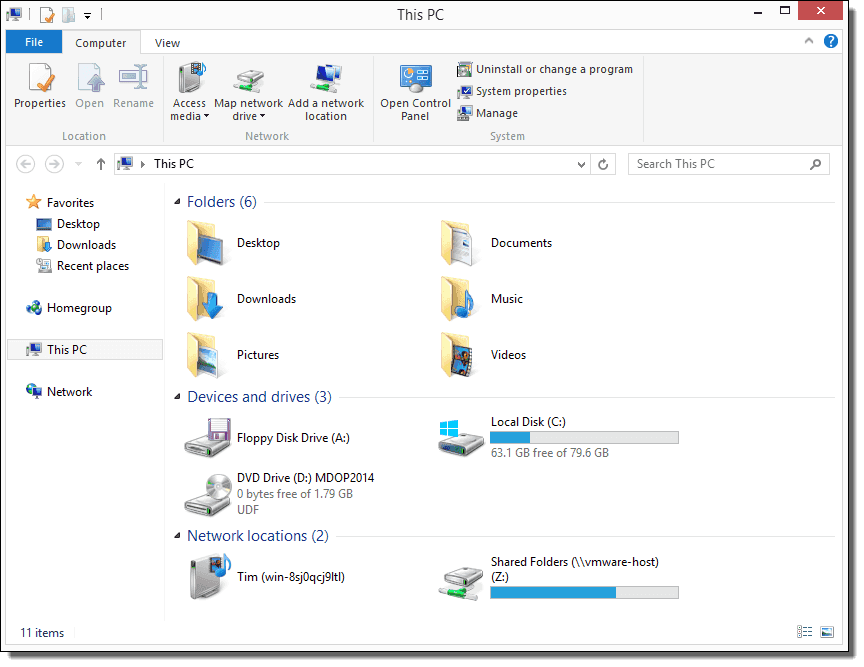
\includegraphics[width=0.85\textwidth]{images/windowsGUI.png}
	\caption{Windows file explorer}
	\label{fig:windows:file}
\end{figure}

The file explorer GUI hides the details of the operations being done by the computer away from the user of the program. This provides simplicity, but it also limits the flexibility of what a user can do with the computer. Moreover, it means that users can only interact with a system that has a GUI installed. This doesn’t include computers without a standard operating system, servers, or computers that a user is connected to remotely. \\

%The \textbf{command line} is a program you can access through the GUI of a linux machine. 
On the other hand, the \textbf{command line} is a program that  interface directly with the operating system and issue commands that it can understand. The command line can be accessed directly through the monitor without a GUI. In fact, before the invention of the GUI, the command line was the only way to interact with computers!  On modern computers, the command line can be accessed through the GUI of a linux machine. \\
%The command line is also installed on servers without a GUI and can be accessed directly through monitors (this was the only way to interact with computers before the invention of the GUI).\\

The command line allows the user to issue a broader range of commands and interact with computers without a graphical interface. 
%The command line lets users interface directly with the operating system and issue commands that it can understand. 
This increases the range of the commands that the user can issue, giving them more flexibility to perform complex and custom tasks. \\

\section{Linux command line}

We will discuss the command line used in the Linux operating system because it is one of the most common and intuitive command lines. \\

\begin{center}
    \begin{tabular}{| l | p{75mm} | }
      \hline
      Command & Description \\ \hline
      ls & List all the files in the current directory \\ \hline
      touch & Create a new file \\ \hline
      cd [name] & Changes the current directory to [name] \\ \hline
      mkdir [name] & Create a new directory within the current directory named [name] \\ \hline
      man [command] & Display the manual for a [command] \\ \hline
      cat [file] & Display the contents of [file] in the terminal \\ \hline
      mv [file] [location] & Moves [file] to the directory [location]. \\ \hline 
%      By default it moves file to a different name within the same directory. \\ \hline
      cp [file] [location] & Creates a new file with identical contents to the [file] specified in a new [location]. If a path for the file isn’t given, it will make a copy of the file in the same directory. \\ \hline
    \end{tabular}
\end{center}
  
  A folder in Linux is referred to as a \textbf{directory}. When you open a command line, you are located in a certain directory within the file system. All commands that you issue that relate to interacting with the file system like creating files, editing files, or renaming files will be issued in the context of this directory. This is like navigating to a particular folder within the GUI file explorer and completing all your operations relative to that folder.

\begin{figure}
	\centering
	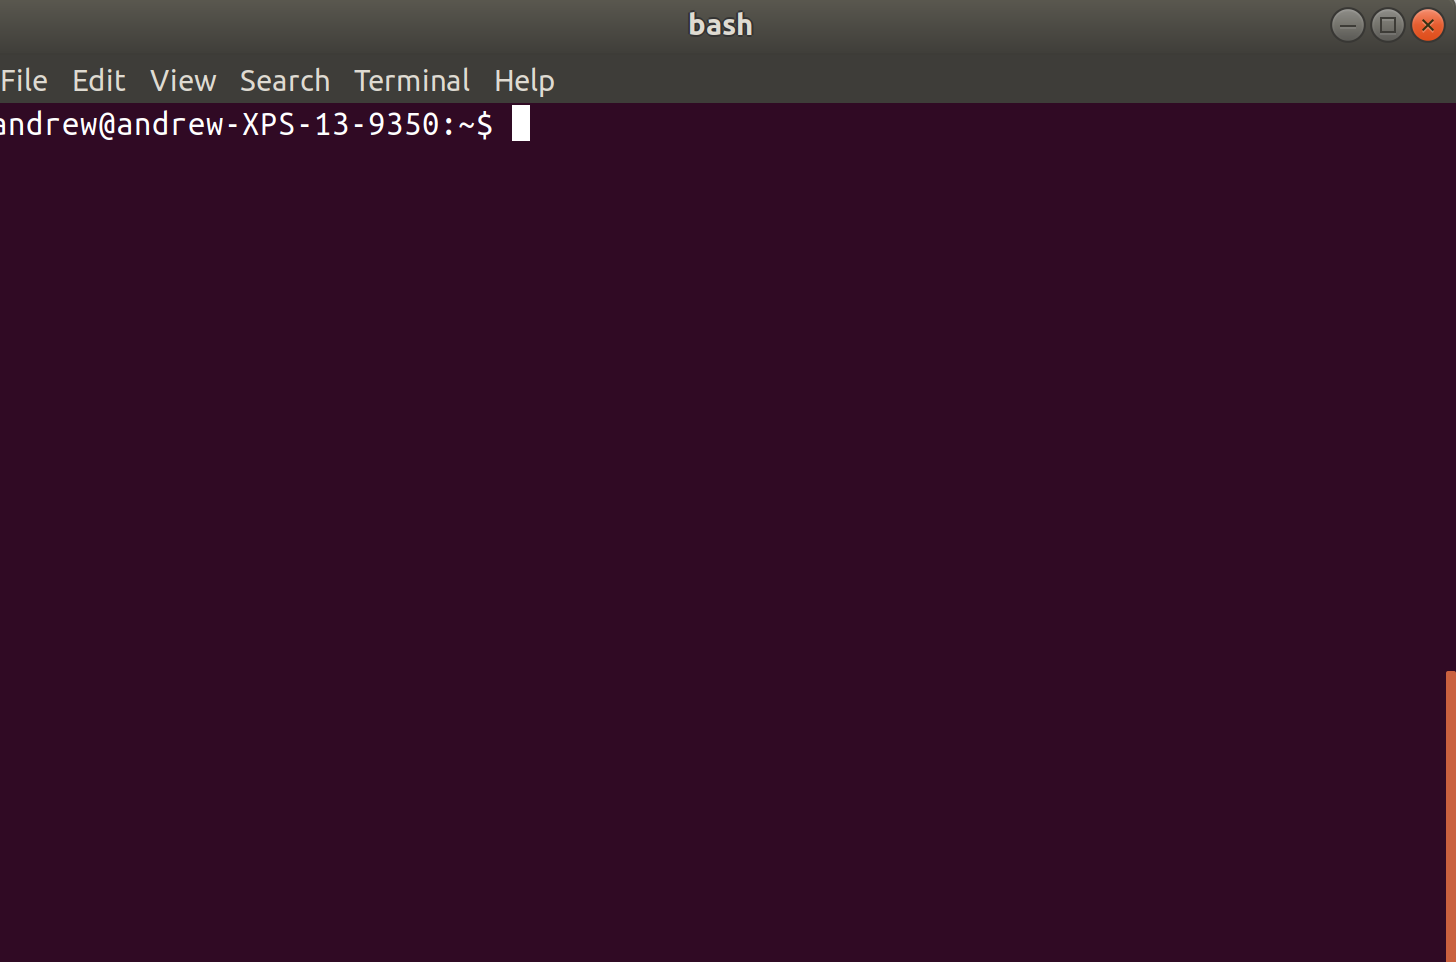
\includegraphics[width=0.85\textwidth]{images/commandLineOne.png}
	\caption{Linux command line}
	\label{fig:linux:one}
\end{figure}

Figure \ref{fig:linux:one} shows the command line interface for a Linux computer. The prompt shown is where the user can type commands. By default it prepends the user’s name, the name of the computer, and a dollar sign. The white rectangle represents the location of my cursor prompting the user to enter commands. \\

For example, Figure \ref{fig:linux:two} displays an example of creating a new directory called commandLineLearning (using the `mkdir` command) and then going inside the commandLineLearning directory (using the `cd` command). This is like making a new folder within an existing folder in the window’s file explorer, and then going inside that folder. \\

In Figure \ref{fig:linux:two}, the $\sim$ sign prepending the command represents the user’s home directory. The home directory is the outer most folder for that user’s account on the server or machine. \\

\begin{figure}
	\centering
	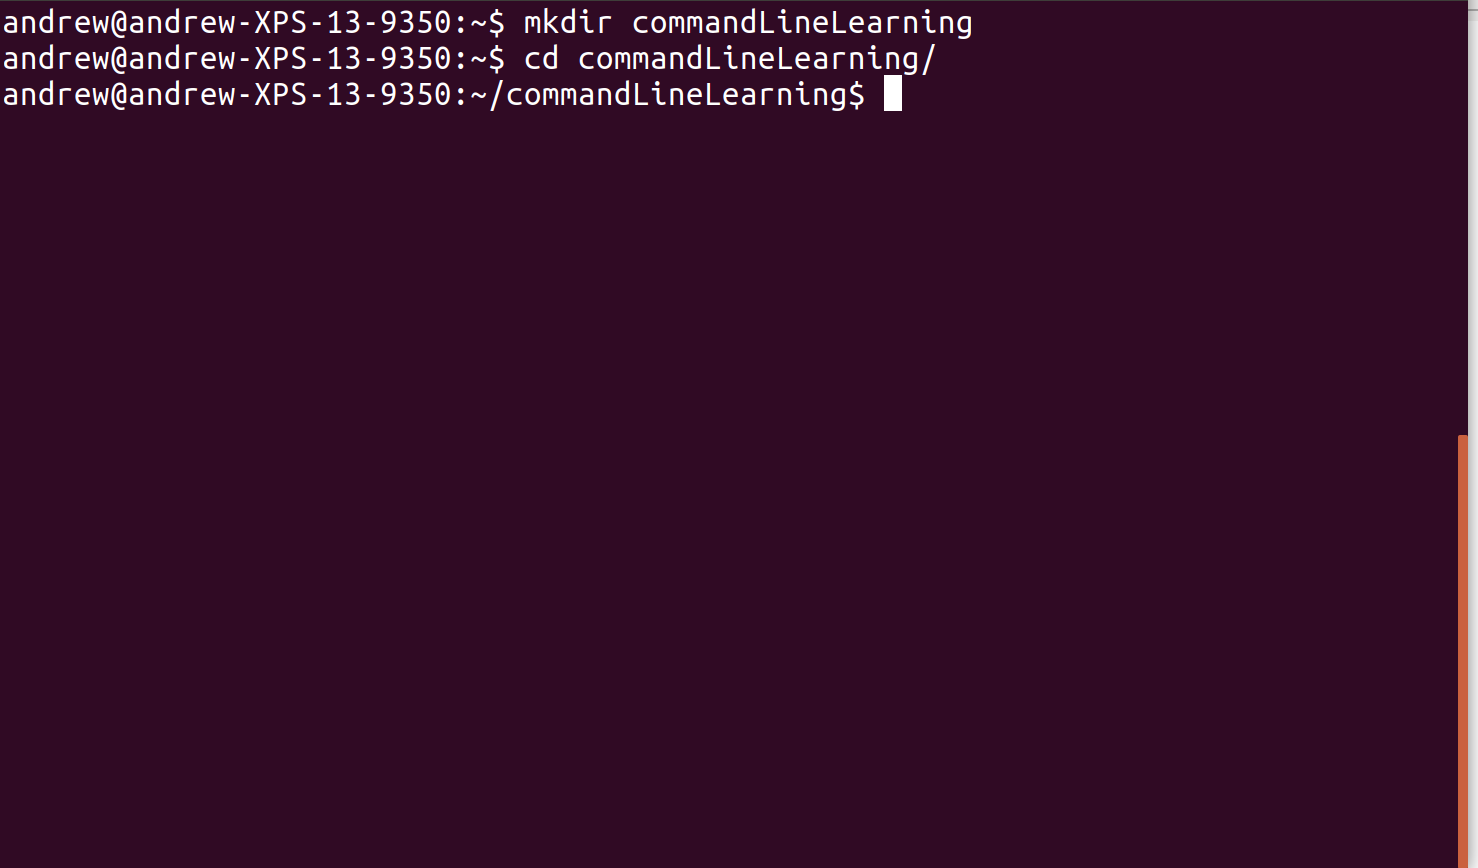
\includegraphics[width=0.85\textwidth]{images/commandLineTwo.png}
	\caption{Creating a directory}
	\label{fig:linux:two}
\end{figure}

\begin{figure}
	\centering
	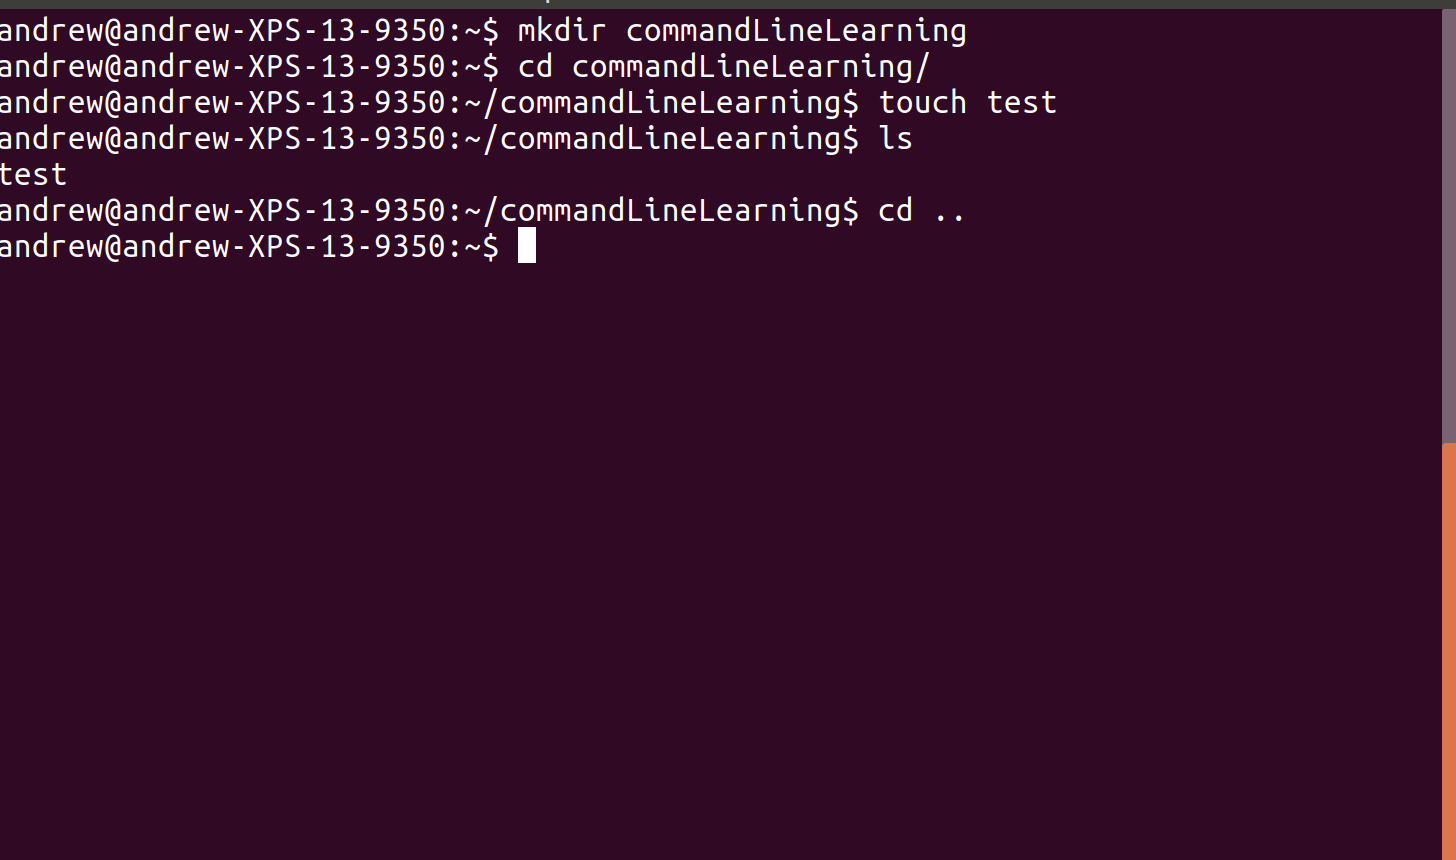
\includegraphics[width=0.85\textwidth]{images/commandLineThree.png}
	\caption{Listing files and navigating}
	\label{fig:linux:three}
\end{figure}

\begin{figure}[ht]
	\centering
	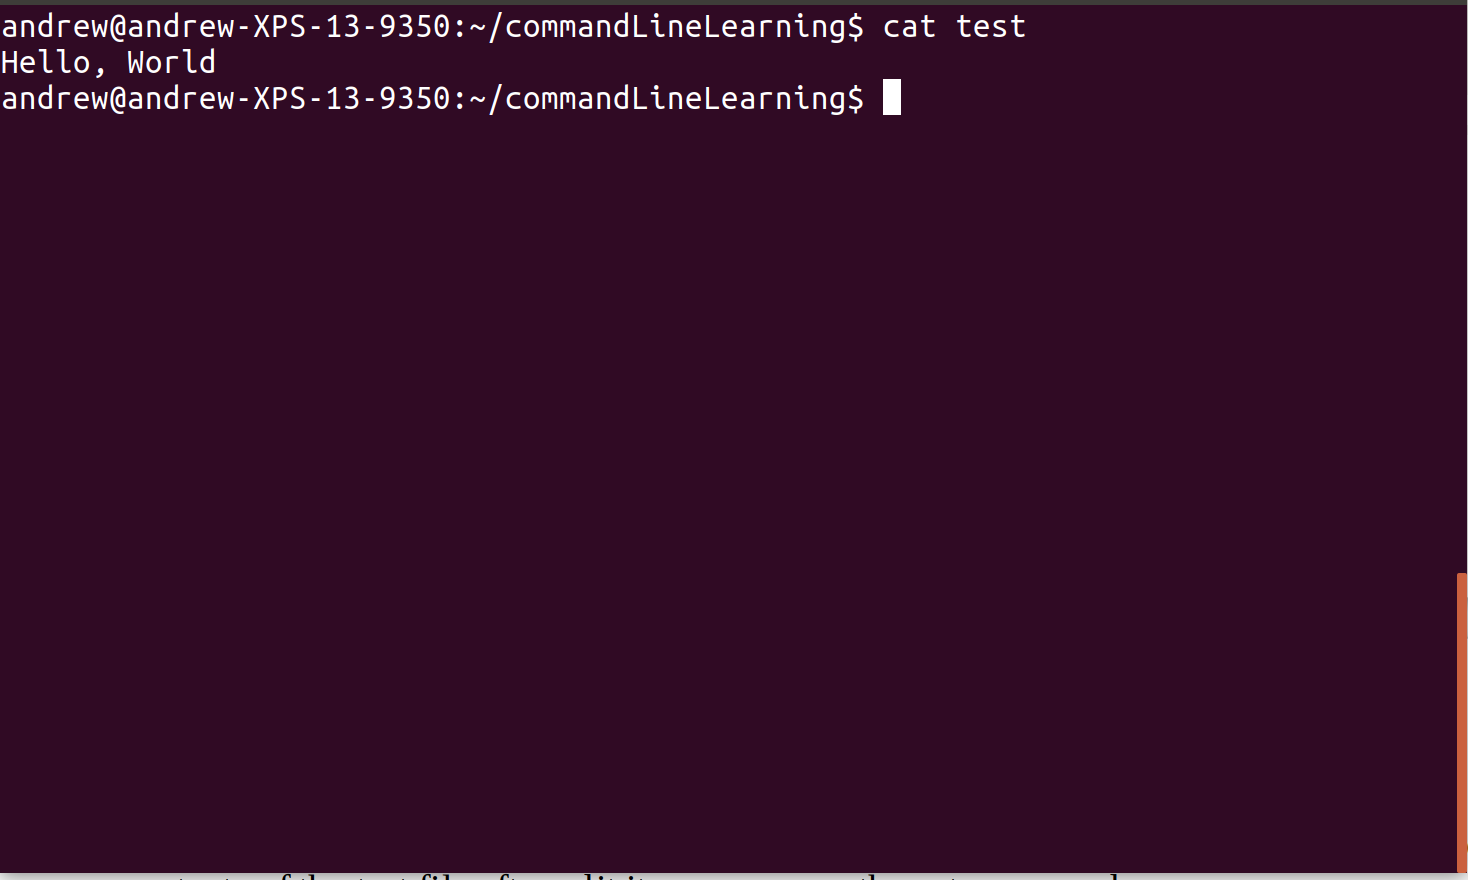
\includegraphics[width=0.85\textwidth]{images/commandLineFour.png}
	\caption{Cat command example}
	\label{fig:linux:four}
\end{figure}

If we want to create a file inside the commandLineLearning directory, we can use the ‘touch’ command to create a new file. If we want to see the files in the directory, we can use the ‘ls’ command to list all of the files inside the current directory. Finally, if we want to move back to the directory we were in before, we can use the ‘cd’ command with the parameters ‘..’ to move to the directory my current directory is contained within. In Linux, ‘..’ refers to the directory that contains the current directory, or the parent directory. These commands are summarized in Figure \ref{fig:linux:three}. \\

Try these commands out! You can edit the contents of test using any file editing software. To view the contents of the test file after you edit it, you can use the `cat` command (Figure \ref{fig:linux:four}). \\

%\newpage

\section{Lab: Running Hello World in the Command Line}

In this exercise, we will create a ``Hello World'' program in Java and run it --- only using the command line.

\begin{enumerate}
\item 
First, open the command line. 
\item Run the command \codeblock{cd $\sim$} which will move you to inside the \codeblock{$\sim$} folder. The \codeblock{$\sim$}  folder refers to your home directory.
\item
Next run \codeblock{cd Desktop}. This will take you to your Desktop. Afterwards, run \codeblock{cd CS103}, which will take you to your CS103 folder from Chapter 2. See Figure \ref{fig:linux:exercise:zero2}.

After running these commands, you might notice that the left side of your window (before the \$ sign) changes. This is because it indicates your current directory, which has changed from \codeblock{Desktop} to \codeblock{CS103}.

\begin{figure}[ht]
	\centering
	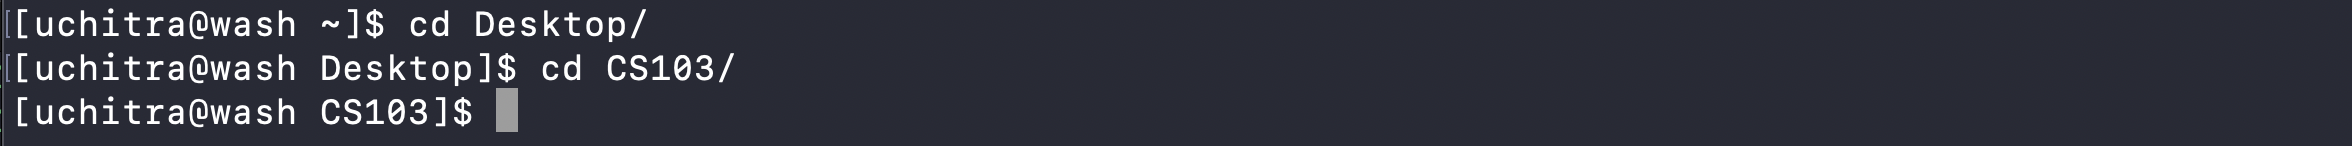
\includegraphics[width=0.85\textwidth]{images/commandLineExercise_zero2}
	\caption{Navigating to the \codeblock{CS103} folder you created from Chapter 2.}
	\label{fig:linux:exercise:zero2}
\end{figure}

\item
Next, run \codeblock{mkdir Chapter\_8}. This will create a folder called \codeblock{Chapter\_8} inside the \codeblock{CS103} folder. 

To check that you created this folder, run \codeblock{ls}. This will show all of the contents in your current folder. Verify that \codeblock{Chapter\_8} is listed. See Figure \ref{fig:linux:exercise:one2}.

\begin{figure}[ht]
	\centering
	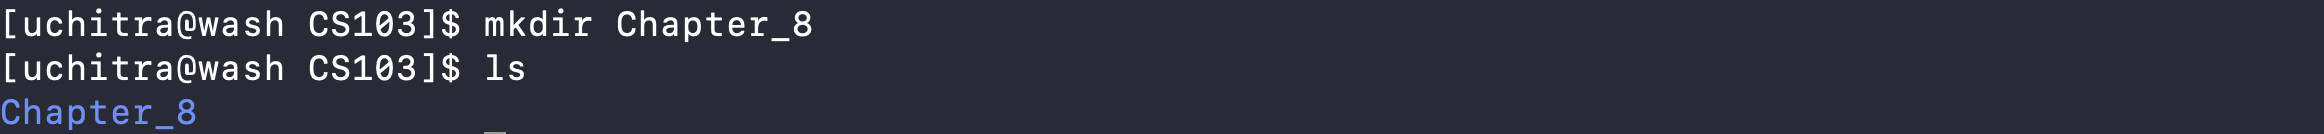
\includegraphics[width=0.85\textwidth]{images/commandLineExercise_one2}
	\caption{Creating and going inside the \codeblock{Chapter\_8} folder.}
	\label{fig:linux:exercise:one2}
\end{figure}

\item 
Then run \codeblock{cd Chapter\_8}. This will take you inside the \codeblock{Chapter\_8} folder.

\item
Next, we will copy the Hello World file we created in Chapter 2 into the \codeblock{Chapter\_8} folder we just created.

To do this, run the command 

\codeblock{cp ~/Desktop/CS103/Chapter\_2/HelloWorld.java ~/Desktop/CS103/Chapter\_8/}

To understand why this command works, recall that running \codeblock{cp [file] [location]} makes a copy of \codeblock{[file]} in \codeblock{[location]}. In the cp command above, \codeblock{[file]} is the path to the Hello World file from Chapter 2, and \codeblock{[location]} is the \codeblock{Chapter\_8} folder you just created.

To check that the \codeblock{cp} command worked successfully, run the \codeblock{ls} command. This will display all of the files in your current folder, which is the \codeblock{Chapter\_8} folder. You should see a file called \codeblock{HelloWorld.java}. See Figure \ref{fig:linux:exercise:two2}.

\begin{figure}[ht]
	\centering
	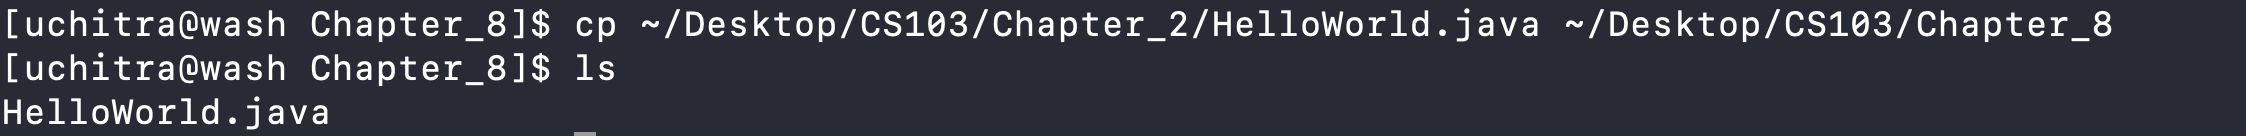
\includegraphics[width=0.85\textwidth]{images/commandLineExercise_two2}
	\caption{Copying the HelloWorld.java file from Chapter 2 into your \codeblock{Chapter\_8} folder.}
	\label{fig:linux:exercise:two2}
\end{figure}

\item
To verify that your code matches what you wrote in Chapter 2, run \codeblock{cat HelloWorld.java}. This will print out the contents of \codeblock{HelloWorld.java}.  See Figure \ref{fig:linux:exercise:three2}.

\begin{figure}[ht]
	\centering
	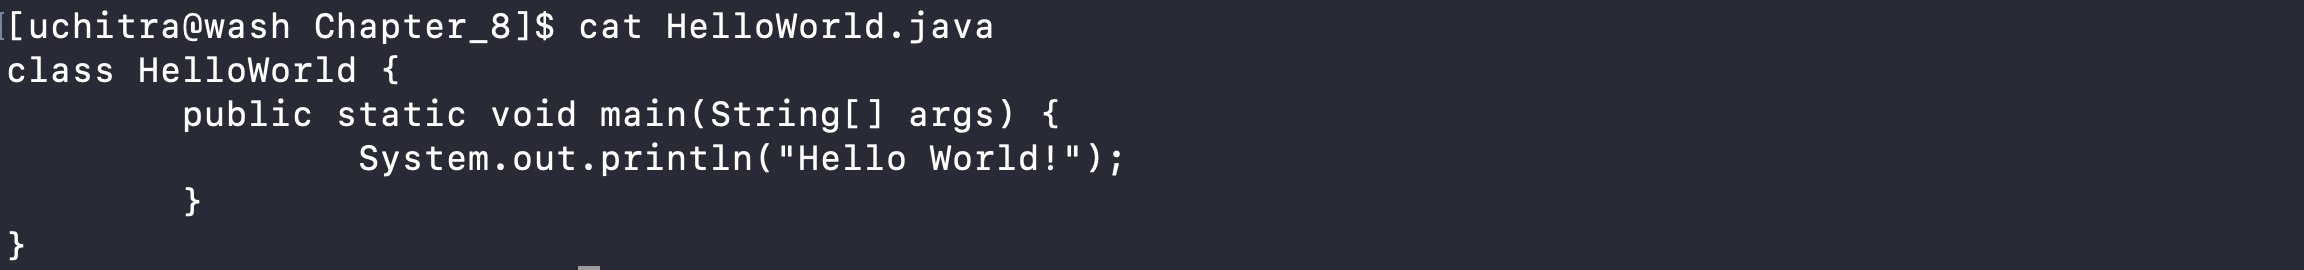
\includegraphics[width=0.85\textwidth]{images/commandLineExercise_three2}
	\caption{Running \codeblock{cat HelloWorld.java} to see the contents of \codeblock{HelloWorld.java}. Your code may look different depending on what you did in Chapter 2.}
	\label{fig:linux:exercise:three2}
\end{figure}

\item Now let's run our Hello World code! First, we have to compile the java file by running \codeblock{javac HelloWorld.java}. This will create a file named \codeblock{HelloWorld.class}. This file contains the bytecode instructions for the computer to run our program. See Figure \ref{fig:linux:exercise:four2}.

\begin{figure}[ht]
	\centering
	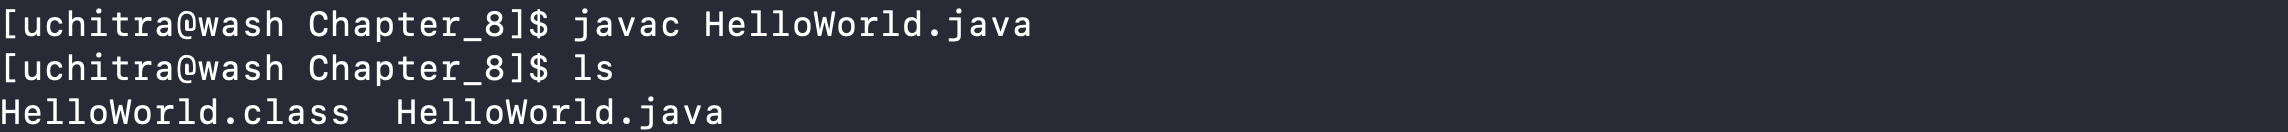
\includegraphics[width=0.85\textwidth]{images/commandLineExercise_four2}
	\caption{Running \codeblock{javac HelloWorld.java}. Running \codeblock{ls} afterwards shows that a \codeblock{HelloWorld.class} file was created.}
	\label{fig:linux:exercise:four2}
\end{figure}

\item Next, run \codeblock{java HelloWorld}. Here, the \codeblock{HelloWorld} refers to the name of the ``class" in the java file. If everything is correct, the result should be the phrase ``Hello World!", as shown in Figure \ref{fig:linux:exercise:five2}.

\begin{figure}[ht]
	\centering
	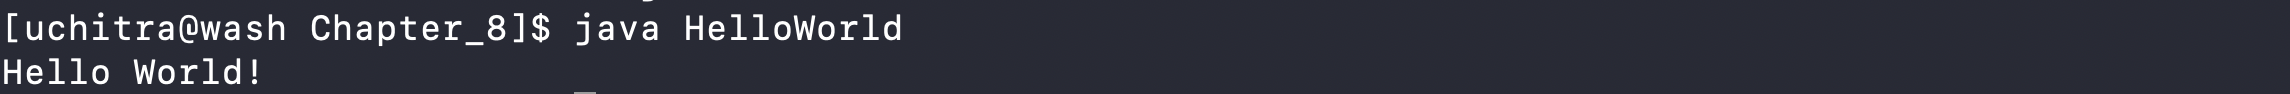
\includegraphics[width=0.85\textwidth]{images/commandLineExercise_five2}
	\caption{Running \codeblock{java HelloWorld.java}. The output of our program, which prints ``Hello World!", should appear below.}
	\label{fig:linux:exercise:five2}
\end{figure}

\item Congrats! You finished the lab! If you have extra time, check if someone sitting nearby needs any help.

\end{enumerate}
\newpage
\exercisesection

\begin{exercise}
Name three different programming languages.
\end{exercise}

\begin{exercise}
Name the process that turns your code into instructions that a computer can execute.
\end{exercise}

\begin{exercise}
Name an example of a GUI.
\end{exercise}

\begin{exercise}
Which command in the command line lets you to create a new directory?
\end{exercise}

\begin{exercise}
Which command in the command line lets you view the contents of a file?
\end{exercise}

\referencessection

Stack Overflow Developer Survey 2019. (n.d.).
        \pagebreak
	\chapter{Networks I: Protocols}

Computing devices have been in use for thousands of years, at least since the invention of the Sumerican abacus between four and five thousand years ago. Even as computers became more sophisticated, a long process culminating in the development of transistor-based digital computers, they remained specialized machines, largely for use in government or business settings. The explosion in personal computing, which has flooded the planet with billions of computers that pervade almost every aspect of society, coincided roughly with the development of computer networking and the Internet. Communicating via computers -- with friends, news outlets, vendors, banks, or even artificial intelligence systems -- has revolutionized the way the world works.

In the next two chapters, we'll learn how computer networks work, from the wires in the ground up to the more familiar technologies in a browser or email client. The Internet is one of the largest and most complex machines ever built, so we certainly won't be able to cover every aspect of it, but we'll focus on a few important topics. After reading the next two chapters, you should be able to tell a story about what happens when you open a website or send an email, and understand how to get under the hood and see how different pieces are working together to complete the task.

In this chapter, we'll focus specifically on the \emph{protocols} that allow computers to communicate with one another. We'll cover what a protocol is, and why detailed protocols are important for ensuring reliable networking. In the next chapter, we'll look at how these protocols work together and allow us to build large computer networks, including the global Internet.

Understanding networks is both interesting and very practical. Many companies look for Internet Technology or IT specialists who understand how networks work. Taking a test like the Network+ certification or A+ certification allows access to these jobs. These tests are knowledge based, so you don’t need practical experience to do well on them. They qualify you for entry level positions that pay around \$50,000 a year. If you're interested in preparing for these exams, there are many books that can help you prepare. For instance, ``CompTIA A+ Certification All-in-One Exam Guide, Ninth Edition (Exams 220-901 \& 220-902).''

\section{Protocols}

Long before there were computers, there were protocols. A protocol is a set of rules and procedures that specify how two entities should interact. In particular, protocols can apply to people, in the form of social protocols. These can be simple -- for example, there is an unspoken protocol regarding shaking someone's hand -- or quite complex, as in the protocol for diplomatic exchanges between different countries. In fact, the US Department of State employs a Chief of Protocol, whose office is tasked with ensuring that visiting diplomats and heads of state are appropriately welcomed and not offended by any ``breach of protocol.''

Rather than delve into complex diplomatic protocol, let's consider the simple example: the ``handshake protocol.'' It's so easy to shake someone's hand that we might not realize how many rules and procedures we follow when we do it. Here are a few possible ``breaches of protocol'' that could occur when Alice shakes Bob's hand.
\begin{itemize}
    \item Alice extends a left hand, while Bob extends a right hand.
    \item After locking hands, Alice refuses to let go for a full 15 seconds.
    \item After locking hands, Alice lets go immediately without pausing for a shake.
    \item Alice refuses to make eye contact for the duration of the handshake.
    \item Alice shakes her hand left to right, or forward and backward.
    \item Alice makes no effort to grip Bob's hand, leaving the handshake loose.
    \item Alice uses a ``death grip,'' causing Bob discomfort.
    \item Alice extends her arm fully and locks her elbow, keeping Bob at as great a distance as possible.
    \item Alice barely extends her arm, forcing Bob to stand very close.
    \item Alice sneezes into her hand immediately before initiating the handshake.
\end{itemize}
Any of these examples would cause some problems; many would lead Bob to wonder if Alice had ever shaken hands before, while a few might leave Bob offended or wondering if Alice does not like Bob. Clearly it is important that Alice and Bob abide by some rules so that their handshake goes smoothly and gives a friendly message to both parties.

How might we construct such a set of rules, or a protocol? It would be helpful to first divide the above gaffes into a few categories. One way to categorize them is chronologically: there are potential problems in 3 stages: initiating the handshake, completing the handshake, and terminating the handshake.

Let's first write a protocol for initiating a handshake. The two parties need to come to an appropriate distance, verify that their hands are clean, make eye contact, and both extend the same hand. We can condense this into a step-by-step procedure:

\begin{graybox}
{\Large Handshake Initiation}
\begin{enumerate}
    \item Verify that your right hand is acceptably clean, and maintain this status until handshake termination.
    \item Look at the other party, and wait for eye contact to be established.
    \item After making eye contact, approach the other party and come to within about one arm length apart.
    \item Extend your right hand to the halfway point between you and the other party, at about waist height, and orient your hand so that your open palm is facing left.
    \item Wait for the other party to extend their hand likewise.
\end{enumerate}
\end{graybox}

There are a surprising number of steps for something we all do almost unconsciously! 

\begin{exercise}
    Write similarly detailed protocols for Handshake Completion and Handshake Termination. Make sure your protocol eliminates the possibility of any of the gaffes listed above.
\end{exercise}

You might wonder why need to write out these detailed protocols, since handshakes are so obvious. The reason is that computers have no social intuition whatsoever. This is why protocols are important: a computer needs to be told every single step of an interaction as simple as a handshake in order to execute it properly. Building a computer network requires a number of different protocols to establish how messages are sent on wires, routed to the appropriate destination, and more.

One of the most important parts of a protocol is that everyone follows the same one. Some aspects of protocols are completely arbitrary, and it is important for everyone to follow the same arbitrary convention. For example, handshakes could use left hands instead of right hands. Luckily the whole world shakes right hands, but anyone who's tried driving in both the US and UK knows that not all protocols are the same.

For computer networks specifically, in order to ensure that networking protocols are consistent around the world, a body known as the Interent Engineering Task Force (IETF) carefully specifies all the protocols and makes them publicly available. Publications of the IETF are known as Requests For Comments, or RFCs. The name ``Request For Comments'' originated in the early days of computer networking, when the documents were intended for comments and discussion. Nowadays there is a category called standards-track RFCs which specify the standards of the Internet and should be followed by anyone building networking technology.

\section{Network Layers}\label{sec:network:layers}

In the previous section we saw an example of a protocol for initiating a handshake. The protocol was more detailed than you might have expected, but it also didn't include all the details. For example, let's delve into step 2: ``Look at the other party, and wait for eye contact to be established.'' First, what does it mean to ``look at the other party''? This requires identifying the location of another human, and sending motor signals to the neck and to the eyeballs in such a way as to orient them in the direction of the other human's eyeballs. If we were to include all these details, our protocol would become extremely complex and hard to follow.

In real life, we avoid this complexity by never even thinking about these details of movement, facial recognition, and the like. Our brains can automatically send the right signals to our muscles, interpret signals from our senses, and so on. We say that the brain is segmented into two layers: conscious and unconscious. The conscious layer sends high-level signals, such as the command ``Look at Bob,'' to the unconscious layer. The unconscious layer is responsible for parsing those commands and executing them by sending the right signals to muscles. This \textbf{layered architecture} allows the protocols to remain simple by referring to the capabilities of lower layers. As we will see later, computer networks also use a layered architecture.

%Communication networks also use a layered architecture. We will come to the layers that make up the Internet in a moment, but long before the Internet we had the postal system. 
Another example of a layered architecture that is similar to a computer network is the postal system. The postal system is built up from layers, and in many ways the Internet is simply a much faster and more automated version of the same layers. Let's consider the following example of a letter being sent from Alice at Acme, Inc. to Bob at Boxes, Inc.:

\begin{enumerate}
    \item Alice tells her employee, Jane, to order 50 new boxes. Jane drafts a letter to Bob at Boxes, Inc. which says ``Please send 50 boxes.'' She seals the letter in an envelope, opens her address book and copies down Bob's mailing address, and drops the envelope off at the company mailroom. A worker in the mailroom sees that the letter is addressed to a destination outside Acme, Inc., and so he places the envelope in a postal box outside.
    \item A postal worker picks up the envelop from the postal box, and sees that the letter is addressed to a location outside the city. He brings the letter to the local post office, and places it into a bin to be sorted.
    \item Another postal worker picks up the envelope from the bin, and puts it on a mail truck destined for Bob's city.
    \item The mail truck drives along a highway from Alice's city to Bob's city, and gives the letter to the post office there.
    \item A postal worker in Bob's city carries the envelope to Boxes, Inc., and places it in their mailbox.
    \item A worker in the mailroom sees the envelope addressed to Bob. She brings it to Bob's office and puts it on his desk where he'll see it.
    \item Bob reads the letter, and asks an employee to begin producing 50 new boxes for Acme, Inc.
\end{enumerate}

There's a lot going on here -- when you think about it, it's amazing that the letter managed to reach Bob at all, given everything that had to go correctly. The trick here is the layered architecture. Alice didn't need to know what highway the letter would be carried on, and the mail truck driver didn't need to know where to find Bob's address. Everyone in the pipeline has a specialty, and no one needs to understand the full process for it to work well. Figure \ref{fig:layer_mail} shows the different steps arranged in layers, from Alice and Bob at the top down to the truck driver at the bottom.

\begin{figure}
    \centering
    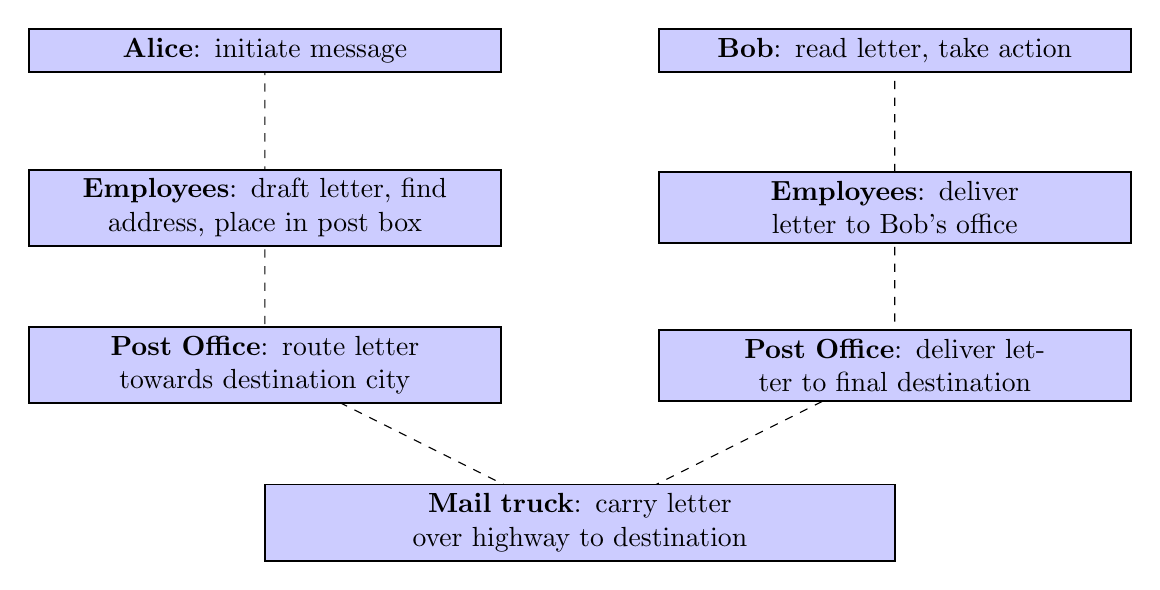
\begin{tikzpicture}[layer/.style={fill=blue!20,minimum width=6cm,align=center,text width=5.5cm,draw=black,solid,line width=.25mm}]
        \draw[dashed,-latex] (-4, 4) node[layer] {\textbf{Alice}: initiate message} --
        (-4, 2) node[layer] {\textbf{Employees}: draft letter, find address, place in post box} --
        (-4, 0) node[layer] {\textbf{Post Office}: route letter towards destination city} --
        (0, -2) node[layer,minimum width=8cm,text width=7.5cm] {\textbf{Mail truck}: carry letter over highway to destination} --
        (4, 0)  node[layer] {\textbf{Post Office}: deliver letter to final destination} --
        (4, 2)  node[layer] {\textbf{Employees}: deliver letter to Bob's office} --
        (4, 4)  node[layer] {\textbf{Bob}: read letter, take action};
    \end{tikzpicture}
    \caption{Layers of the postal system.}
    \label{fig:layer_mail}
\end{figure}

These layers all have counterparts in the Internet. At the top, we have the \emph{application layer}: programs which rely on the Internet and know how to initiate messages, much like Alice and Bob. The application layer relies on the \emph{transport layer} to determine an address where the messages should go, just as Alice relied on Jane to find Bob's mailing address. The transport layer relies on the \emph{Internet layer} to use the address to send the message to the right location, just as the Post Office routed Alice's letter to Bob's city. Finally, the transport layer relies on the \emph{link layer} to physically transmit data over wires or wireless protocols, just as the Post Office relies on mail trucks to move envelopes.

This set of four layers is commonly known as TCP/IP, named for the Transmission Control Protocol (TCP) which commonly runs the transport layer, and the Internet Protocol (IP) which commonly runs the Internet layer. The following sections contain more details on each of the layers and the protocols they use. You should always keep in mind that these layers work together just like the layers of the postal system work together.

\subsection{Application Layer}

The application layer is the highest layer of TCP/IP. It consists of various protocols that specify how to send different types of data over the Internet. You might have heard of one of these protocols, HTTP. HTTP stands for HyperText Transfer Protocol. It comes at the beginning of a web address. When you type \ic{http://www.google.com}, you're telling your computer to use HTTP to access \ic{www.google.com}.

There are many other protocols in the application layer. HTTPS is a secure version of HTTP, which uses security protocols we'll discuss in Section \ref{sec:network:security}. Another popular protocol is SSH, or Secure Shell, which programmers use to access the command line (see previous chapter) on another machine. The file transfer protocol, or FTP, is used for exchanging files between different computers. A variety of protocols, such as POP3, IMAP, and SMTP, are used for exchanging emails.

When the application layer receives data from the transport layer, it needs to know which protocol it was sent with. In order to sort out all the different data, the application layer uses \emph{ports}. All Internet communications happen over some numbered port. For example, HTTP uses port 80. When you load \ic{http://www.google.com}, your computer sends a request to Google over port 80, telling Google to load the home page. Google sends its home page back over port 80. Table \ref{tab:common_ports} lists the most commonly used protocols and the ports they use.

\begin{table}
    \centering
    \begin{tabular}{lll}
        Protocol & Port & Usage \\
        \hline
        HTTP & 80 & Web traffic \\
        HTTPS & 443 & Secure web traffic \\
        FTP & 21 & File transfer \\
        SSH & 22 & Remote shell access \\
        IMAP & 993 & Receiving email \\
        SMTP & 587 & Sending email
    \end{tabular}
    \caption{Commonly used Internet protocols.}
    \label{tab:common_ports}
\end{table}

If you write a program that uses the Internet, you will interact primarily with the application layer. A very common example is writing a program which runs on a web server. A web server is a computer which is connected to the Internet, and runs a program that constantly listens for incoming communications on ports 80 and 443 -- the ports used for the World Wide Web. When it receives a request, it will run a program and send the output of that program back to the requester. Every website is hosted by a web server, which knows how to send the data of the website to anyone who requests it.

A simple and famous example is \ic{isitfriday.net}. This website is hosted by a server which listens for requests. When it gets a request for \ic{isitfriday.net}, it will run a program which checks if it is Friday (you'll learn how to use ``if'' logic in programs in the next chapter). If it is Friday, it sends back a website that says ``Yes.'' Otherwise, it sends back a website that says ``Not yet.''

\subsection{Transport Layer}

When the application layer is ready to transmit a message, it will pass it down to the transport layer. By far the most common transport layer protocol is TCP, for Transmission Control Protocol. We will focus on TCP in this section. Another common protocol in the transport layer is TLS, for Transport Layer Security, which runs alongside TCP. We will discuss TLS more in Section \ref{sec:network:security}.

When TCP is asked to transfer a message, it will prepare to divide up the message and send it piece by piece over the network. The individual pieces are called \emph{packets}. These packets are relatively small, about a kilobyte. For reference, if you are sending an image over TCP, an average-sized image would typically be broken into a few thousand packets before being transferred. 

The reason for dividing up the message is that a major role of TCP is to guarantee reliability. 
%While the application layer assumes that its message will be sent in full and without errors, 
The Internet layer does not guarantee accurate or successful transmission, so it is the job of the transport layer to ensure robust communication. By breaking a message into small packets, TCP helps to reduce the chance that the entire message fails to transmit, since most of the packets will reach the destination. In addition, if a packet does fail to transmit, it doesn't take too much time to recover, since TCP can re-send the relatively small packet.

In addition to providing reliability, TCP is responsible for initiating connections between two computers. When TCP receives a request to transfer a message to a destination, it will first complete a ``handshake'' with that destination. The goal of the handshake is to establish that both parties are connected to the Internet and ready and willing to communicate with one another. In addition, the parties need to synchronize a \emph{sequence number} which specifies the numbers that will label subsequent packets.

We have already thought about handshakes between humans in some detail, so now let's delve into how TCP facilitates handshakes between computers. If humans were communicating using a TCP-style handshake, the conversation might look like this:
\begin{enumerate}
    \item Alice says to Bob, ``Let's start talking. I'll send some packets, starting with this one, \#3874.''
    \item Bob says to Alice, ``I hear you Alice, and I'm looking forward to packet \#3875. My packets will start with this one, \#8452.''
    \item Alice says to Bob, ``Great, I'm looking forward to packet \#8453.''
\end{enumerate}
This is the \emph{three-way handshake} model. First, Alice notifies Bob of her intent to communicate and synchronizes her sequence number. Then Bob sends an acknowledgement of Alice's sequence number, and also synchronizes his own sequence number. Finally, Alice acknowledge's Bob's sequence number, and then they are ready to communicate.

There are two kinds of messages being sent in the handshake, synchronization and acknowledgement. These are typically abbreviated as \ic{SYN} and \ic{ACK}. The TCP handshake protocol works as follows.
\begin{graybox}
{\Large TCP Handshake}
\begin{enumerate}
    \item $A$ generates a random number $x$. $A$ sends $\boxed{\ic{SYN}\ x}$ to $B$.
    \item $B$ generates a random number $y$. $B$ sends $\boxed{\ic{ACK}\ x+1}$ to $A$, and then sends $\boxed{\ic{SYN}\ y}$ to $A$.
    \item $A$ sends $\boxed{\ic{ACK}\ y+1}$ to $B$.
\end{enumerate}
\end{graybox}

\subsection{Internet Layer}

Perhaps the most interesting layer of the TCP/IP stack is the Internet layer, which almost always consists of the Internet Protocol (IP). This layer corresponds to the Post Office in our analogy: it is responsible for routing data where it needs to go. Just as the Post Office uses mailing addresses to specify locations, the Internet layer uses IP addresses to specify computers on the network.

An IP address is a sequence of 32 bits, grouped into blocks of 8. When they are written out, the groups of 8 bits are converted to decimal numbers between 0 and 255. The groups are separated by dots, so sometimes an IP address is referred to as a ``dotted quad.'' For example, the IP address \ic{172.217.15.78} points to the server which hosts \ic{www.google.com}. These addresses are stored in a sort of phone book called the Domain Name System, or DNS. When you type a website into your browser, it will first look up its IP address in the Domain Name System, and then request that IP address over the network.

When the Internet layer receives a packet from the transport layer for transmission, it will look at the IP address of the destination. It knows how to find a server which is closer to that destination. For example, if a server in New York City sees a packet destined for an IP address in Washington, DC., it might decide to forward that packet to a server in Philadelphia, PA.

You can view this process yourself using a Unix utility called \ic{traceroute}. Open a terminal and type \ic{traceroute} followed by any website. You'll see how the Internet Protocol routes your packets through different servers in order to reach their destination. For example, below is the route from a personal computer to \ic{youtube.com}. The address in the last line, \ic{172.217.12.238}, specifies the location of one of YouTube's servers.

\label{code:traceroute}
\begin{monospace}
# traceroute youtube.com
    1  192.168.1.1 (192.168.1.1)  0.448 ms  0.958 ms  0.966 ms
    2  * * *
    3  ae1312-21.ARTNVAFC-MSE01-AA-IE1.verizon-gni.net (100.41.21.152)  7.779 ms  7.766 ms  7.628 ms
    4  0.ae10.GW13.IAD8.ALTER.NET (140.222.225.219)  9.139 ms  9.117 ms  9.082 ms
    5  72.14.218.232 (72.14.218.232)  8.507 ms  7.277 ms  4.378 ms
    6  * * *
    7  216.239.54.106 (216.239.54.106)  4.779 ms 108.170.232.0 (108.170.232.0)  12.022 ms 108.170.246.33 (108.170.246.33)  16.086 ms
    8  108.170.246.67 (108.170.246.67)  12.976 ms 108.170.232.19 (108.170.232.19)  12.769 ms 108.170.246.66 (108.170.246.66)  10.935 ms
    9  iad30s15-in-f14.1e100.net (172.217.12.238)  10.570 ms 216.239.47.127 (216.239.47.127)  16.793 ms iad30s15-in-f14.1e100.net (172.217.12.238)  10.485 ms
\end{monospace}

The IP addresses we've described all correspond to version 4 of the Internet Protocol, or IPv4. There are about four billion unique IPv4 addresses, which seemed like plenty at the time of its creation. However, the growth of the Internet and the proliferation of mobile devices has led to the exhaustion of almost all IPv4 addresses. In order to ensure that the Internet can continue to grow, a transition to IPv6, which provides for many more addresses, is slowly taking place.

In the transport layer, we delved into the step-by-step procedure used for handshaking. These sorts of procedures are one important aspect of the protocols that run networks. Another important aspect is the format in which data is sent. The link layer, which we'll come to in the next section, can only send sequences of bits -- zeroes and ones -- so it is important for both parties to agree on which bits mean what.

To give an example of this, we will look inside the packets sent by IPv4. You should not try to memorize the following, but instead try to appreciate the importance of having a detailed packet structure.

An IP packet is divided into its \emph{header} and the \emph{data}. The header contains information about how the packet is being transmitted, while the data is the actual contents of the packet. The format of IPv4 headers is shown in Table \ref{tab:ipv4}. The various segments specify the following information.
\begin{itemize}
    \item \textbf{Version}: the first four bits specify the version of IP being used. For IPv4, these bits are always \ic{0100}, binary for 4.
    \item \textbf{IHL}: this is the Internet Header Length. This specifies the number of 32 bit blocks, called ``words,'' used by the header. In Table \ref{tab:ipv4} we show a header with 5 words, so these bits are \ic{0101}. This is almost always the case, although it is possible to have a larger IHL value and include additional data in the header.
    \item \textbf{DSCP}: this stands for Differentiated Services Code Point. These bits are used to specify the type of service for the packet. This allows the network to give priority to some packets, such as those used for voice or video calling, which need to arrive as quickly as possible.
    \item \textbf{ECN}: this stands for Explicit Congestion Notification. This allows the network to flag packets which are experiencing congestion along their routes.
    \item \textbf{Total Length}: this specifies the total length of the packet, in bytes including both the header and data. Since it is 16 bits, the maximum value is $2^{16}-1 = 65535$ bytes, or about 64 KB.
    \item \textbf{Fragmentation Data}: these bits are used to group packets which have been fragmented due to a maximum transmission size imposed by the link layer.
    \item \textbf{Time to Live}: this keeps track of how many hops a packet has made through the network. Every time the packet is forwarded along a new link in the network, this value is decreased by one. If it hits zero, the packet is dropped and the sender is notified. This is how the \ic{traceroute} utility works: it sends packets with small Time to Live values, and waits for the notifications to see where the packet was after one hop, two hops, etc.
    \item \textbf{Protocol}: this specifies the transport layer protocol which is making use of IP. For example, for TCP the protocol value is set to 6.
    \item \textbf{Header Checksum}: these bits are used for correcting errors in the header. The idea of a ``checksum'' is encoded in the word: we could imagine transmitting a stream of bits, followed by a few bits that count the number of ones in the original stream. If a zero was flipped to a one, or a one was flipped to a zero, then the receiver will notice that the checksum does not match and can ask for the packet to be resent. In practice a checksum is a more complicated function of the bits, but the idea is the same.
    \item \textbf{Source IP Address}: this is the address of the device sending the packet. Note that it spans 32 bits, since an IPv4 address consists of four numbers each from 0 -- 255, which require 8 bits each.
    \item \textbf{Destination IP Address}: this is the address of the device meant to receive the packet.
\end{itemize}

\begingroup
\tabcolsep=0.05cm
\begin{table}
    \centering
    \footnotesize
    \begin{tabular}{|c|c|c|c|c|c|c|c|c|c|c|c|c|c|c|c|c|c|c|c|c|c|c|c|c|c|c|c|c|c|c|c|c|}
        \hline
        Bit & 0 & 1 & 2 & 3 & 4 & 5 & 6 & 7 & 8 & 9 & 10 & 11 & 12 & 13 & 14 & 15 & 16 & 17 & 18 & 19 & 20 & 21 & 22 & 23 & 24 & 25 & 26 & 27 & 28 & 29 & 30 & 31 \\
        \hline
        0 & \multicolumn{4}{c|}{Version} & \multicolumn{4}{c|}{IHL} & \multicolumn{6}{c|}{DSCP} & \multicolumn{2}{c|}{ECN} & \multicolumn{16}{c|}{Total Length} \\
        \hline
        32 & \multicolumn{32}{c|}{Fragmentation Data} \\
        \hline
        64 & \multicolumn{8}{c|}{Time to Live} & \multicolumn{8}{c|}{Protocol} & \multicolumn{16}{c|}{Header Checksum} \\
        \hline
        96 & \multicolumn{32}{c|}{Source IP Address} \\
        \hline
        128 & \multicolumn{32}{c|}{Destination IP Address} \\
        \hline
    \end{tabular}
    \caption{The IPv4 header format.}
    \label{tab:ipv4}
\end{table}
\endgroup

\subsection{Link Layer}

Finally, we come to the actual nuts and bolts of the Internet: how are individual pieces of data sent across the network? This part of networking is handled by the link layer.

There are two main link layer technologies you will encounter. The first is Ethernet, which is used for wired Internet connections. An Ethernet cable, also known as an RJ-45 cable, is shown in Figure \ref{fig:ethernet}. Each end of the cable has an 8-pin connector. Inside the cable, a twisted pair of wires can carry signals in both directions without having them collide with each other.

\begin{figure}
    \centering
    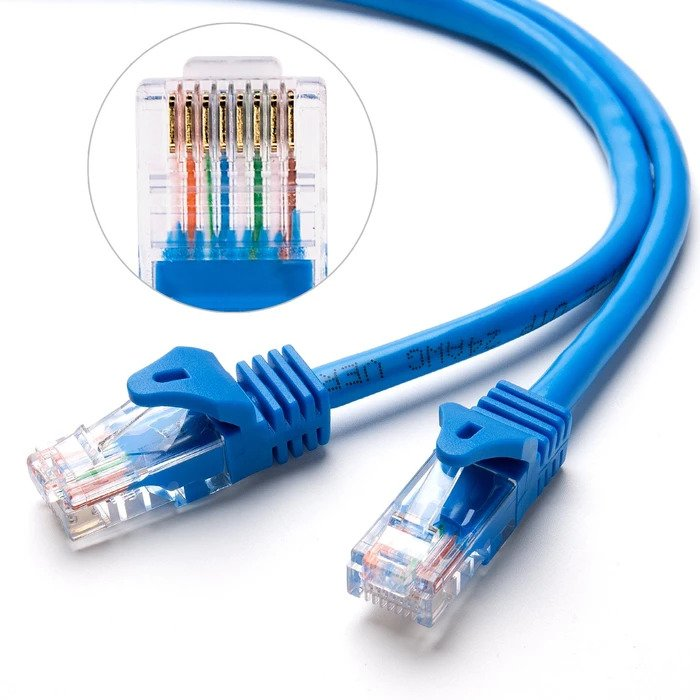
\includegraphics[width=.6\linewidth]{images/ethernet.jpg}
    \caption{An Ethernet cable used to network computers together.}
    \label{fig:ethernet}
\end{figure}

The other primary link layer technology is 802.11, more commonly known as Wi-Fi. With a wired network, signals can be sorted into separate wires so they don't overlap, but over a wireless network signals are broadcast and have the potential to interfere with one another. In order to prevent this, Wi-Fi is designed to allow devices to operate at slightly different frequencies which are arranged into channels.

There are two major variants of Wi-Fi: 2.4 gigahertz (GHz) and 5 GHz. These are two different frequency bands. Within each of them there are multiple channels. At 2.4 GHz, which was the first frequency available for Wi-Fi, there are 11 channels. However, the channels overlap with one another, so it is best for devices to use channels 1, 6, and 11, reducing the efffective number of channels down to 3. The newer 5 GHz protocol alleviates this problem by making hundreds of channels available. Most new devices can operate at either 2.4 GHz or 5 GHz, but some older devices only support 2.4 GHz.

The details of link layer technologies are complex, but luckily you rarely have to deal with them directly. In most cases, Ethernet or Wi-Fi have been engineered to the point where little effort is required to make them work properly, and you can focus on other layers of the network while trusting that signals are being carried appropriately by the link layer.


\section{Network Security}\label{sec:network:security}

One of the most important issues with computer networks is security. The Internet is frequently used for transmitting confidential messages, facilitating financial transactions, and other applications where security is paramount. For this reason,there are protocols dedicated to ensuring that the Internet can be secure. The most common such protocol is Transport Layer Security (TLS), which is a successor to an older protocol called Secure Sockets Layer (SSL). TLS is implemented at the transport layer of a network. Web traffic which uses TLS/SSL security is sent using the HTTPS protocol at the application layer, rather than the unsecured HTTP protocol.

Another common network security application is a Virtual Private Network, or VPN. A VPN allows computers connected to different LANs to communicate over the Internet as if they belonged to the same LAN. This is often used by companies to allow employees to access private resources even when they are away from the office. Security is very important for a VPN, and it can be provided using TLS or other protocols.

The details of TLS are complicated, and we will not get into them here. Instead, we will cover what exactly security means in a network setting, and look at three goals of any secure network: privacy, authenticity, and reliability. Achieving these goals requires using tools from cryptography, which you may learn about in a future course.

\subsection{Privacy}

When two parties want to securely transmit a message, one of their most straightforward goals is privacy. The two parties do not want a third party to be able to lisen in on their communication.

Following a standard convention in cryptography, we will denote the two parties by Alice and Bob, and the adversarial third party by Carol. Alice is sending a message to Bob, and Carol wants to listen in. Since network signals travel over cables, Carol could listen in to the signal by physically tapping into a wire. Even more easily, on a wireless network, all signals are broadcast over the air and can be received by anyone who wants to listen.

In order to protect their messages from being read by Carol, Alice and Bob use an encryption algorithm. Alice and Bob have some shared key, and when Alice wants to send a message, she first uses her key to turn the plain text of the message into a cipher text. If the algorithm is secure, then the cipher text cannot be converted back to the plain text without knowledge of the key. This way, if Carol manages to read the message, she will only see nonsensical cipher text. Only Bob, who has the key, can produce the plain text.

A key issue here is how Alice and Bob come to have the same key. If Alice tells Bob her key over the network, then Carol could retrieve the key and use it to decrypt all future messages. This is a fundamental problem in cryptography called the key-sharing problem. It is solved using a technique called public key cryptography. In TLS, public key cryptography is implemented using either the RSA algorithm, or a more sophisticated method called elliptic curve cryptography (ECC). These algorithms allow Alice and Bob to generate shared keys which Carol cannot intercept.

\subsection{Authenticity}

Even if Carol cannot read messages sent between Alice and Bob, she can still do damage. One potential attack would be for Carol to impersonate Alice, by sending a message to Bob which says it comes from Alice. This is why TLS must also protect the authenticity of messages: if a message says it comes from Alice, Bob needs some way of verifying that this is actually the case.

The public key cryptography algorithms used for ensuring privacy can also provide authenticity. In these algorithms, every party on the network has a private key which is never shared with anyone. This private key is important for generating the shared keys used for encrypting messages. It can also be used to generate a ``digital signature,'' which could only be produced by someone in possession of the private key. As long as the private key has never been shared, a digital signature can provide a guarantee of authenticity.

\subsection{Integrity}

Finally, even if Carol cannot read messages or impersonate Alice or Bob, she could try to modify one of their messages. This is called a man-in-the-middle (MITM) attack, where Carol intercepts Alice's communications, edits them, and then forwards them to Bob with Alice's signature intact.

To protect against this, TLS uses a message authentication code (MAC) which is sent along with any message. This is a short code sent with the message, which depends on the shared key and on the message. If the algorithms are secure, then it should be nearly impossible to generate a MAC without knowledge of both the shared key and the message. When Bob receives the message along with the MAC, he verifies that the MAC is correct. If it is not, then he knows the message has been altered in transit and discards it.

\subsection{Security versus Trust}

An enormous amount of expertise, testing, and iteration has gone into making TLS secure. However, it is still relatively common to hear about security problems on the Internet. Where do these problems come from?

In this context, it is important to recognize a key difference between security and trust. Network security provided by TLS achieves the three goals outlined above: privacy, authenticity, and integrity. When Alice communicates with Bob, she can be sure that only Bob can read her messages, that messages she receives from Bob really come from Bob, and that the messages have not been altered in transit. However, \emph{TLS does not guarantee that Alice can trust Bob}.

There are many ways in which Bob could be unreliable. For example, Bob could be attempting to execute a phishing attack by impersonating someone else. TLS guarantees that Bob cannot truly impersonate \ic{facebook.com}, but he could own \ic{fcebook.com} and, using TLS security, provide a website that looks just like \ic{facebook.com} and asks for your login credentials. If you provide them to \ic{fcebook.com}, then Bob could read your password and log into your actual Facebook account.

Even if Bob is not malicious, he could be irresponsible. For example, if Bob runs an online vendor which collects credit card information to make payments, it is crucial that Bob takes appropriate security measures on his local network to protect that credit card information from becoming known to an attacker. TLS does not guarantee that Bob has taken the necessary precautions. Many of the most substantial security problems arise on the Internet when many customers have trusted a vendor like Bob with their personal details like credit card numbers, and Bob suffers a data breach, putting this data into the wrong hands.

Network security is an evolving field as companies and governments work to protect against these sorts of vulnerabilities. There are many opportunities for employment in this area, as organizations increasingly need to rely on dedicated security professionals in order to keep their data and their clients' data safe.

\exercisesection

\begin{exercise}
    Put the following layers in order from top to bottom, and give an example of a protocol or technology used in each layer.
    \begin{itemize}
        \item Transport Layer
        \item Link Layer
        \item Application Layer
        \item Internet Layer
    \end{itemize}
\end{exercise}

\begin{exercise}
    What protocol is used as part of HTTPS in order to ensure secure transmission of data? List the three goals of this protocol and give a description of the kind of attack each goal seeks to prevent. Then give an example of an attack which would not be prevented by this protocol.
\end{exercise}

% this seems way too hard

%\begin{exercise}
%    Identify all of the following blocks of IP addresses which contain 48.192.72.86. (\emph{Hint:} you may want to write out each address block in binary.)
%    \begin{itemize}
%        \item 48.192.0.0/12
%        \item 48.192.0.0/16
%        \item 48.192.0.0/20
%        \item 48.0.0.0/4
%        \item 48.0.0.0/8
%        \item 48.0.0.0/12
%        \item 48.192.64.0/20
%        \item 48.192.64.0/24
%    \end{itemize}
%\end{exercise}

\begin{exercise}
    In a TCP handshake, Alice initiates by sending $\boxed{\ic{SYN}\ 895}$ to Bob. Give an example of the remaining steps that could take place in this handshake.
\end{exercise}

\begin{exercise}
    What is the main advantage of 5 GHz WiFi over 2.4 GHz WiFi? Why is 2.4 GHz WiFi still in use?
\end{exercise}
	\pagebreak
	\chapter{Networks}

Computing devices have been in use for thousands of years, at least since the invention of the Sumerican abacus between four and five thousand years ago. Even as computers became more sophisticated, a long process culminating in the development of transistor-based digital computers, they remained specialized machines, largely for use in government or business settings. The explosion in personal computing, which has flooded the planet with billions of computers that pervade almost every aspect of society, coincided roughly with the development of computer networking and the Internet. Communicating via computers -- with friends, news outlets, vendors, banks, or even artificial intelligence systems -- has revolutionized the way the world works.

In this chapter, we'll learn how computer networks work, from the wires in the ground up to the more familiar technologies in a browser or email client. The Internet is one of the largest and most complex machines ever built, so we certainly won't be able to cover every aspect of it, but we'll focus on a few important topics. After reading, you should be able to tell a story about what happens when you open a website or send an email, and understand how to get under the hood and see how different pieces are working together to complete the task.

In addition to its inherent interest, understanding networks is very practical. Many companies look for Internet Technology or IT specialists who understand how networks work. Taking a test like the Network+ certification or A+ certification allows access to these jobs. These tests are knowledge based, so you don’t need practical experience to do well on them. They qualify you for entry level positions that pay around \$50,000 a year. If you're interested in preparing for these exams, there are many books that can help you prepare. For instance, ``CompTIA A+ Certification All-in-One Exam Guide, Ninth Edition (Exams 220-901 \& 220-902).''

\section{Network Layers}\label{sec:network:layers}

Before the Internet, the most popular method of communication at a distance was the postal system. In many ways, the Internet is a much faster and more automated version of the postal system. In particular, the Internet is built up from several different layers. Let's consider the following example of a letter being sent from Alice at Acme, Inc. to Bob at Boxes, Inc.:

\begin{enumerate}
    \item Alice tells her employee, Jane, to order 50 new boxes. Jane drafts a letter to Bob at Boxes, Inc.: ``Please send 50 boxes.'' She seals it in an envelope, opens her address book and copies down Bob's mailing address, and drops the envelope off at the company mailroom. A worker in the mailroom sees that the letter is addressed to a destination outside Acme, Inc., and so he places the envelope in a postal box outside.
    \item A postal worker picks up the envelop from the postal box, and sees that the letter is addressed to a location outside the city. He brings the letter to the local post office, and places it into a bin to be sorted.
    \item Another postal worker picks up the envelope from the bin, and puts it on a mail truck destined for Bob's city.
    \item The mail truck drives along a highway from Alice's city to Bob's city, and gives the letter to the post office there.
    \item A postal worker in Bob's city carries the envelope to Boxes, Inc., and places it in their mailbox.
    \item A worker in the mailroom sees the envelope addressed to Bob. She brings it to Bob's office and puts it on his desk where he'll see it.
    \item Bob reads the letter, and asks an employee to begin producing 50 new boxes for Acme, Inc.
\end{enumerate}

There's a lot going on here -- when you think about it, it's amazing that the letter managed to reach Bob at all, given everything that had to go correctly. The trick here is the layered architecture. Alice didn't need to know what highway the letter would be carried on, and the mail truck driver didn't need to know where to find Bob's address. Everyone in the pipeline has a specialty, and no one needs to understand the full process for it to work well. Figure \ref{fig:layer_mail} shows the different steps arranged in layers, from Alice and Bob at the top down to the truck driver at the bottom.

\begin{figure}
    \centering
    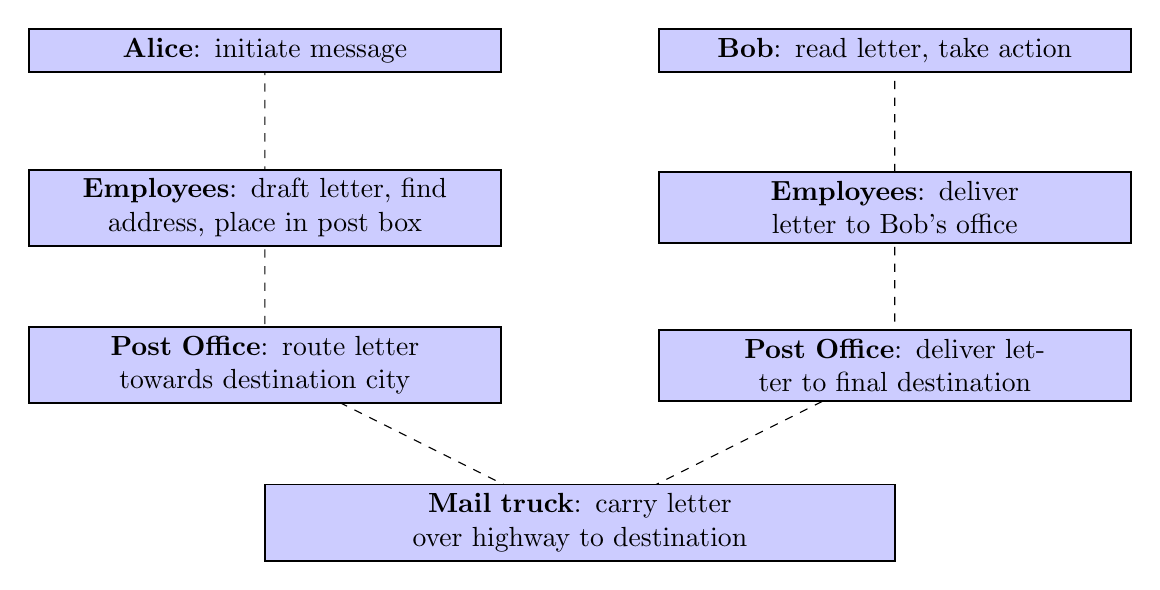
\begin{tikzpicture}[layer/.style={fill=blue!20,minimum width=6cm,align=center,text width=5.5cm,draw=black,solid,line width=.25mm}]
        \draw[dashed,-latex] (-4, 4) node[layer] {\textbf{Alice}: initiate message} --
        (-4, 2) node[layer] {\textbf{Employees}: draft letter, find address, place in post box} --
        (-4, 0) node[layer] {\textbf{Post Office}: route letter towards destination city} --
        (0, -2) node[layer,minimum width=8cm,text width=7.5cm] {\textbf{Mail truck}: carry letter over highway to destination} --
        (4, 0)  node[layer] {\textbf{Post Office}: deliver letter to final destination} --
        (4, 2)  node[layer] {\textbf{Employees}: deliver letter to Bob's office} --
        (4, 4)  node[layer] {\textbf{Bob}: read letter, take action};
    \end{tikzpicture}
    \caption{Layers of the postal system.}
    \label{fig:layer_mail}
\end{figure}

These layers all have counterparts in the Internet. At the top, we have the \emph{application layer}: programs which rely on the Internet and know how to initiate messages, much like Alice and Bob. The application layer relies on the \emph{transport layer} to determine an address where the messages should go, just as Alice relied on Jane to find Bob's mailing address. The transport layer relies on the \emph{Internet layer} to use the address to send the message to the right location, just as the Post Office routed Alice's letter to Bob's city. Finally, the transport layer relies on the \emph{link layer} to physically transmit data over wires or wireless protocols, just as the Post Office relies on mail trucks to move envelopes.

This set of four layers is commonly known as TCP/IP, named for the Transmission Control Protocol (TCP) which commonly runs the transport layer, and the Internet Protocol (IP) which commonly runs the Internet layer. The following sections contain more details on each of the layers. You should always keep in mind that these layers work together just like the layers of the postal system work together.

\subsection{Application Layer}

The application layer is the highest layer of TCP/IP. It consists of various protocols that specify how to send different types of data over the Internet. You might have heard of one of these protocols, HTTP. HTTP stands for HyperText Transfer Protocol. It comes at the beginning of a web address. When you type \texttt{http://www.google.com}, you're telling your computer to use HTTP to access \texttt{www.google.com}.

There are many other protocols in the application layer. HTTPS is a secure version of HTTP, which we'll discuss in Section \ref{sec:network:security}. Another popular protocol is SSH, or Secure Shell, which programmers use to access a Linux terminal on another Internet-connected machine. The file transfer protocol, or FTP, is used for exchanging files between different computers. A variety of protocols, such as POP3, IMAP, and SMTP, are used for exchanging emails.

When the application layer receives data from the transport layer, it needs to know which protocol it was sent over. In order to sort out all the different data, the application layer uses \emph{ports}. All Internet communications happen over some numbered port. For example, HTTP uses port 80. When you load \texttt{http://www.google.com}, your computer sends the request to Google over port 80. Google sends its home page back over port 80. Table \ref{tab:common_ports} lists the most commonly used protocols and the ports they use.

\begin{table}
    \centering
    \begin{tabular}{lll}
        Protocol & Port & Usage \\
        \hline
        HTTP & 80 & Web traffic \\
        HTTPS & 443 & Secure web traffic \\
        FTP & 21 & File transfer \\
        SSH & 22 & Remote shell access \\
        IMAP & 993 & Receiving email \\
        SMTP & 587 & Sending email
    \end{tabular}
    \caption{Commonly used Internet protocols.}
    \label{tab:common_ports}
\end{table}

If you write a program that uses the Internet, you will interact primarily with the application layer. A very common example is writing a program which runs on a web server. A web server is a computer which is connected to the Internet, and runs a program that constantly listens for incoming communications on ports 80 and 443 -- the ports used for the World Wide Web. When it receives a request, it will run a program and send the output of that program back to the requester. Every website is hosted by a web server, which knows how to send the data of the website to anyone who requests it.

A simple and famous example is \texttt{isitfriday.net}. This website is hosted by a server which listens for requests. When it gets a request for \texttt{isitfriday.net}, it will run a program which checks if it is Friday (you'll learn how to use ``if'' logic in programs in the next chapter). If it is Friday, it sends back a website that says ``Yes.'' Otherwise, it sends back a website that says ``Not yet.''

\subsection{Transport Layer}

When the application layer is ready to transmit a message, it will pass it down to the transport layer. By far the most common transport layer protocol is TCP, for Transmission Control Protocol. We will focus on TCP in this section. Another common protocol in the transport layer is TLS, for Transport Layer Security, which runs alongside TCP. We will discuss TLS more in Section \ref{sec:network:security}.

When TCP receives a request to transfer a message to a destination, it will first complete a ``handshake'' with that destination. The goal of the handshake is to establish that both parties are connected to the Internet and ready and willing to communicate with one another. TCP uses a three-way handshake: first the sender sends a signal to the receiver. The receiver replies with an acknowledgement of the signal, and a signal of its own. Finally, the sender acknowledges the signal from the receiver. At this point TCP can begin transmitting data.

When TCP receives a message for transfer, it will prepare to send it piece by piece over the network. The individual pieces are called \emph{packets}. These packets are relatively small, about a kilobyte. For reference, an average-sized image would typically be broken into a few thousand packets before being transferred. 

The reason for this is that a major role of TCP is to guarantee reliability. The application layer assumes that its message will be sent in full and without errors, while the Internet layer does not guarantee accurate or successful transmission, so it is the job of the transport layer to ensure robust communication. By breaking a message into packets, TCP helps to reduce the chance that any individual packet fails to transmit. In addition, if a packet does fail to transmit, it doesn't take too much time to recover, since TCP can re-send the relatively small packet.

\subsection{Internet Layer}

Perhaps the most interesting layer of the TCP/IP stack is the Internet layer, which almost always consists of the Internet Protocol (IP). This layer corresponds to the Post Office in our analogy: it is responsible for routing data where it needs to go. Just as the Post Office uses mailing addresses to specify locations, the Internet layer uses IP addresses to specify computers on the network.

An IP address is a sequence of 32 bits, grouped into blocks of 8. When they are written out, the groups of 8 bits are converted to decimal numbers between 0 and 255. The groups are separated by dots, so sometimes an IP address is referred to as a ``dotted quad.'' For example, the IP address \texttt{172.217.15.78} points to the server which hosts \texttt{www.google.com}. These addresses are stored in a sort of phone book called the Domain Name System, or DNS. When you type a website into your browser, it will first look up its IP address in the Domain Name System, and then request that IP address over the network.

When the Internet layer receives a packet from the transport layer for transmission, it will look at the IP address of the destination. It knows how to find a server which is closer to that destination. For example, if a server in New York City sees a packet destined for an IP address in Washington, DC., it might decide to forward that packet to a server in Philadelphia, PA.

You can view this process yourself using a Unix utility called \texttt{traceroute}. Open a terminal and type \texttt{traceroute} followed by any website. You'll see how the Internet Protocol routes your packets through different servers in order to reach their destination. For example, below is the route from a personal computer to \texttt{youtube.com}. The address in the last line, \texttt{172.217.12.238}, specifies the location of one of YouTube's servers.

\label{code:traceroute}
\begin{monospace}
# traceroute youtube.com
    1  192.168.1.1 (192.168.1.1)  0.448 ms  0.958 ms  0.966 ms
    2  * * *
    3  ae1312-21.ARTNVAFC-MSE01-AA-IE1.verizon-gni.net (100.41.21.152)  7.779 ms  7.766 ms  7.628 ms
    4  0.ae10.GW13.IAD8.ALTER.NET (140.222.225.219)  9.139 ms  9.117 ms  9.082 ms
    5  72.14.218.232 (72.14.218.232)  8.507 ms  7.277 ms  4.378 ms
    6  * * *
    7  216.239.54.106 (216.239.54.106)  4.779 ms 108.170.232.0 (108.170.232.0)  12.022 ms 108.170.246.33 (108.170.246.33)  16.086 ms
    8  108.170.246.67 (108.170.246.67)  12.976 ms 108.170.232.19 (108.170.232.19)  12.769 ms 108.170.246.66 (108.170.246.66)  10.935 ms
    9  iad30s15-in-f14.1e100.net (172.217.12.238)  10.570 ms 216.239.47.127 (216.239.47.127)  16.793 ms iad30s15-in-f14.1e100.net (172.217.12.238)  10.485 ms
\end{monospace}

The IP addresses we've described all correspond to version 4 of the Internet Protocol, or IPv4. There are about four billion unique IPv4 addresses, which seemed like plenty at the time of its creation. However, the growth of the Internet and the proliferation of mobile devices has led to the exhaustion of almost all IPv4 addresses. In order to ensure that the Internet can continue to grow, a transition to IPv6, which provides for many more addresses, is slowly taking place.

\subsection{Link Layer}

Finally, we come to the actual nuts and bolts of the Internet: how are individual pieces of data sent across the network? This part of networking is handled by the link layer.

There are two main link layer technologies you will encounter. The first is Ethernet, which is used for wired Internet connections. An Ethernet cable, also known as an RJ-45 cable, is shown in Figure \ref{fig:ethernet}. Each end of the cable has an 8-pin connector. Inside the cable, a twisted pair of wires can carry signals in both directions without having them collide with each other.

\begin{figure}
    \centering
    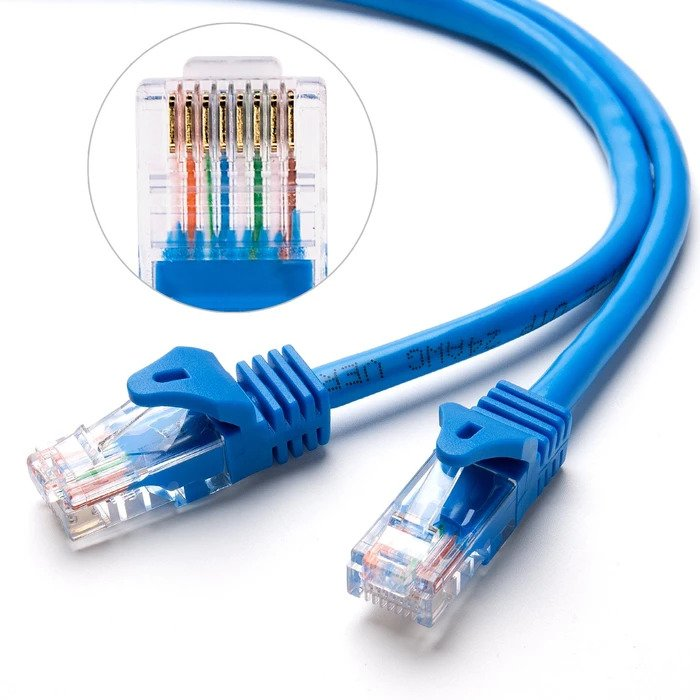
\includegraphics[width=.6\linewidth]{images/ethernet.jpg}
    \caption{An Ethernet cable used to network computers together.}
    \label{fig:ethernet}
\end{figure}

The other primary link layer technology is 802.11, more commonly known as Wi-Fi. With a wired network, signals can be sorted into separate wires so they don't overlap, but over a wireless network signals are broadcast and have the potential to interfere with one another. In order to prevent this, Wi-Fi is designed to allow devices to operate at slightly different frequencies which are arranged into channels.

There are two major variants of Wi-Fi: 2.4 gigahertz (GHz) and 5 GHz. These are two different frequency bands. Within each of them there are multiple channels. At 2.4 GHz, which was the first frequency available for Wi-Fi, there are 11 channels. However, the channels overlap with one another, so it is best for devices to use channels 1, 6, and 11, reducing the efffective number of channels down to 3. The newer 5 GHz protocol alleviates this problem by making hundreds of channels available. Most new devices can operate at either 2.4 GHz or 5 GHz, but some older devices only support 2.4 GHz.

The details of link layer technologies are complex, but luckily you rarely have to deal with them directly. In most cases, Ethernet or Wi-Fi have been engineered to the point where little effort is required to make them work properly, and you can focus on other layers of the network while trusting that signals are being carried appropriately by the link layer.

\section{Local Area Networks}

The network used to connect computers within a single home, business, or organization is called a local area network, or a LAN. Even though most LANs are connected to the outside Internet, they can also be used to allow devices on the same network to connect with each other without going through the Internet. In this section, we will review some concepts of local area networking and discuss using switches to manage network traffic.

\subsection{Network Topology}

When building a LAN, a network engineer has to connect computers either via Ethernet cables or wireless connections. For simplicity, we will focus on wired connections in this section.

In order to allow for a group of computers to communicate with each other, each computer must be able to reach any other computer via some number of hops in the network. The \emph{topology} of the network is the layout of the connections in the network, and this sets how a pair of computers communicates. 

One simple way to allow computers to communicate would be to connect all the computers in a line. Then each computer can communicate with the computers directly adjacent to it. This is called a linear topology, also known as daisy-chaining. Figure \ref{fig:daisy_chain} shows a network with linear topology.

\begin{figure}
    \centering
    \begin{tikzpicture}
        \node at (0,0) (a) {
\includegraphics[width=1cm]{images/computer.png}};
        \node at (3,0) (b) {
\includegraphics[width=1cm]{images/computer.png}};
        \node at (6,0) (c) {
\includegraphics[width=1cm]{images/computer.png}};
        \node at (9,0) (d) {
\includegraphics[width=1cm]{images/computer.png}};
        \draw[dashed,very thick] (a) -- (b) (b) -- (c) (c) -- (d);
    \end{tikzpicture}
    \caption{A network with linear topology.}
    \label{fig:daisy_chain}
\end{figure}

With a linear topology, if a computer wants to send a message to a computer which is not its neighbor, the intermediate computers have to carry the message along. In order to facilitate this, the destination address is included along with a packet. If a computer receives a packet and sees that the destination address is not its own, it will forward the packet along in the direction of the destination address.

One limitation of a linear topology is the difficulty of adding new devices to the network. Every time a new computer is being set up, it would have to be inserted somewhere in the line, causing temporary disruptions in the network. A possible alternative is a bus topology, in which all computers are connected to a central bus line. This layout is shown in Figure \ref{fig:bus}.

\begin{figure}
    \centering
    \begin{tikzpicture}
        \node at (0,0) (a) {
\includegraphics[width=1cm]{images/computer.png}};
        \node at (3,0) (b) {
\includegraphics[width=1cm]{images/computer.png}};
        \node at (6,0) (c) {
\includegraphics[width=1cm]{images/computer.png}};
        \node at (9,0) (d) {
\includegraphics[width=1cm]{images/computer.png}};
        \draw[dashed,very thick] (-1,-1) -- (10,-1);
        \draw[dashed,very thick] (a) -- (0,-1) (b) -- (3,-1) (c) -- (6,-1) (d) -- (9,-1);
    \end{tikzpicture}
    \caption{A network with bus topology.}
    \label{fig:bus}
\end{figure}

With a bus topology, a device can be added to the network simply by linking it to the bus line. When a computer wants to send a message on the network, it specifies the destination address and sends the message to the bus. All other computers receive the message, since they are also on the bus. The computer for which the message was intended can then read the message.

A clear problem with the bus and linear topologies is that several computers on the network are involved whenever two computers have to communicate. In the bus topology in particular, every message is broadcast, so there can be competition for network resources when multiple devices try to send messages at once.

In order to alleviate these difficulties, a network can be arranged in a star topology. In a star topology, shown in Figure \ref{fig:star} all computers are connected to one central device. When a computer wants to send a message, it will send it to the central device, which then forwards it on to the destination address. This way every communication happens with no more than two hops across the network, and only the central device is involved in facilitating communications.

\begin{figure}
    \begin{subfigure}{0.45\linewidth}
        \centering
        \begin{tikzpicture}
            \node at (0,0) (a) {
\includegraphics[width=1cm]{images/computer.png}};
            \node at (90:2) (b) {
\includegraphics[width=1cm]{images/computer.png}};
            \node at (-30:2) (c) {
\includegraphics[width=1cm]{images/computer.png}};
            \node at (-150:2) (d) {
\includegraphics[width=1cm]{images/computer.png}};
            \draw[dashed,very thick] (a) -- (b) (a) -- (c) (a) -- (d);
        \end{tikzpicture}
        \caption{A network with star topology.}
        \label{fig:star}
    \end{subfigure}%
    \hspace{.1\linewidth}%
    \begin{subfigure}{0.45\linewidth}
        \centering
        \begin{tikzpicture}
            \node at (0,0) (a) {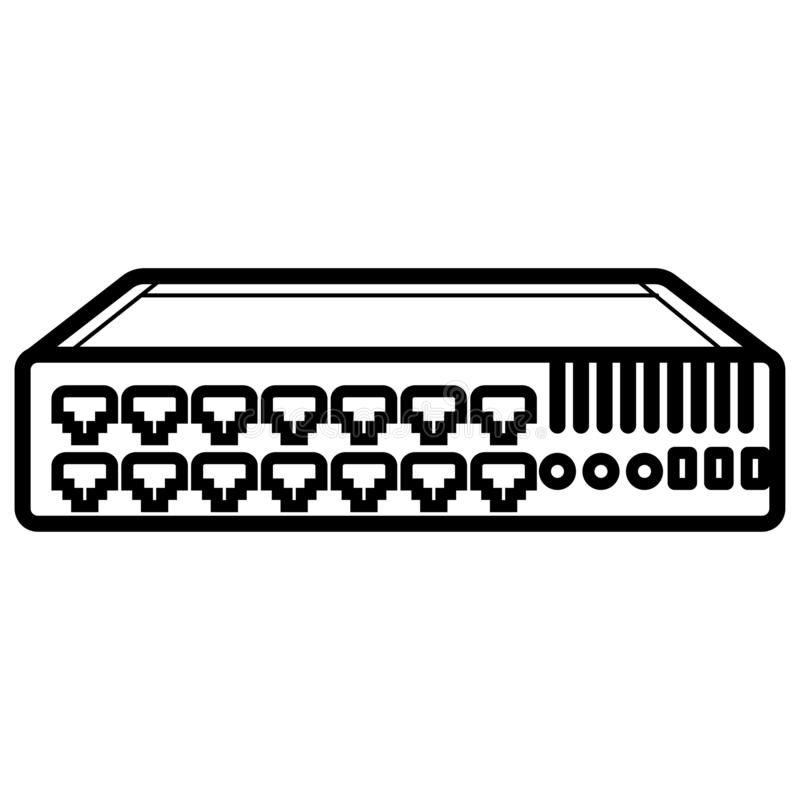
\includegraphics[width=1cm]{images/switch.jpg}};
            \node at (90:2) (b) {
\includegraphics[width=1cm]{images/computer.png}};
            \node at (-30:2) (c) {
\includegraphics[width=1cm]{images/computer.png}};
            \node at (-150:2) (d) {
\includegraphics[width=1cm]{images/computer.png}};
            \draw[dashed,very thick] (a) -- (b) (a) -- (c) (a) -- (d);
        \end{tikzpicture}
        \caption{A switched network.}
        \label{fig:switched}
    \end{subfigure}
    \caption{}
\end{figure}

In a star topology, the central device places an important and unique role. For this reason, it is very often replaced with a specialized network device called a switch. We will discuss switches in the following section.

\subsection{Switches}

A \emph{switch} is a device dedicated to moving packets through a network. It is designed to play the role of the central device in the star topology in Figure \ref{fig:star}. A typical switch may have dozens of Ethernet ports used to connect devices to it. The switch can receive packets from devices through these ports, and knows how to read the destination address of each packet. It forwards every packet along the cable pointing to the destination address, and nowhere else. This way, an Ethernet cable connected to a device is only every carrying packets sent from that device or intended for that device. A switched network is depicted in Figure \ref{fig:switched}.

It is useful to think about a switch in terms of the network layers we covered in Section \ref{sec:network:layers}. A switch is typically an Internet layer device. The Internet layer runs on top of the link layer, and so switches have link layer technology as well: these are the Ethernet ports and cables which allow devices to connect. Once a packet arrives at the switch, it uses the IP protocol in order to forward that packet to the appropriate device on the network. The flow of data from device to device follows the pattern in Figure \ref{fig:switch_layers}.

\begin{figure}
    \centering
    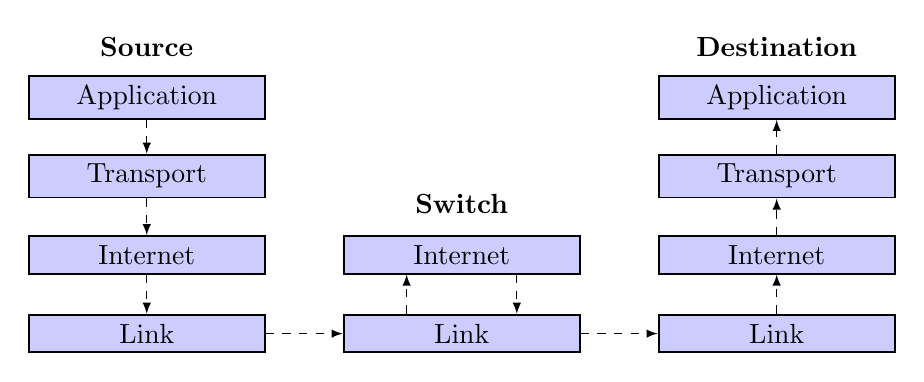
\begin{tikzpicture}[layer/.style={fill=blue!20,minimum width=3cm,align=center,text width=2.5cm,draw=black,solid,line width=.25mm},yscale=0.5]
        \node[above] at (-4, 4.8) {\textbf{Source}};
        \node[layer] at (-4, 4) (a1) {Application};
        \node[layer] at (-4, 2) (a2) {Transport};
        \node[layer] at (-4, 0) (a3) {Internet};
        \node[layer] at (-4, -2) (a4) {Link};

        \node[above] at (0, 0.8) {\textbf{Switch}};
        \node[layer] at (0, 0) (b1) {Internet};
        \node[layer] at (0, -2) (b2) {Link};

        \node[above] at (4, 4.8) {\textbf{Destination}};
        \node[layer] at (4, 4) (c1) {Application};
        \node[layer] at (4, 2) (c2) {Transport};
        \node[layer] at (4, 0) (c3) {Internet};
        \node[layer] at (4, -2) (c4) {Link};

        \draw[dashed,-latex] (a1) -- (a2);
        \draw[dashed,-latex] (a2) -- (a3);
        \draw[dashed,-latex] (a3) -- (a4);
        \draw[dashed,-latex] (a4) -- (b2);
        \draw[dashed,-latex,transform canvas={xshift=-.7cm}] (b2) -- (b1);
        \draw[dashed,-latex,transform canvas={xshift=.7cm}] (b1) -- (b2);
        \draw[dashed,-latex] (b2) -- (c4);
        \draw[dashed,-latex] (c4) -- (c3);
        \draw[dashed,-latex] (c3) -- (c2);
        \draw[dashed,-latex] (c2) -- (c1);
    \end{tikzpicture}
    \caption{The flow of data through network layers in a switched network.}
    \label{fig:switch_layers}
\end{figure}

Imagine a LAN with 50 devices connected to a switch. There are over a thousand different pairs of devices which may need to communicate with another, and the switch enables them to all communicate as if they had a dedicated cable between them, while actually using only 50 cables. This is the essential feature of any network: with relatively few physical connections, they enable an enormous number of potential communication channels. The Internet at large is designed in roughly the same way. We will discuss the details of the organization of the Internet, or more generally any wide area network, in the following section.

\section{Wide Area Networks}

Almost every LAN needs a way of communicating with the outside world. A network at a larger scale than a LAN is called a wide area network, or WAN. By far the most familiar example of a WAN is the Internet, but a WAN need not be this large. For example, a campus or metropolitan area may have its network organized as a WAN.

The link layer technology which carries signals over a WAN is similar to that of a LAN. A WAN typically needs higher capacity Ethernet cables, but the general principles are the same. The primary difference between a LAN and a WAN comes in at the Internet layer, where the IP protocol distinguishes between public and private networks. In this section we will discuss this difference, and the systems and protocols used to connect public networks together.

\subsection{Gateways and Routing}

If you have used a home network, you may be more familiar with routers than switches. This is because a switch is designed to connect all the devices into an area into a local network, but typically we also want to connect a local network to the outside Internet. This is the role of a router. Routers are responsible for connecting different networks together into a larger network.

In a typical setup, several devices on a local network will be connected to a router. The router assigns private IP addresses to each of these devices. Private IP addresses belong to one of three special blocks reserved for this purpose. The most common block is 192.168.*.*, any address ranging from 192.168.0.0 to 192.168.255.255. There are about 65,000 such addresses. A block like this can be written as 192.168.0.0/16, meaning the first 16 bits are fixed and the rest can change. The other private IP address ranges are 172.16.0.0/12, with about 1 million addresses, and 10.0.0.0/8, with about 16 million addresses.

When a device (such as a switch) within the LAN receives a packet, it will look at the destination IP address. If it knows where to route the packet -- that is, if the packet is destined for another device on the local network -- then it will forward the packet appropriately. If it does not know where to route the packet, then it will forward it on to the device designated as the \emph{default gateway} for the network. The default gateway is typically the router.

When the router receives a packet with a destination address outside the local network, it knows how to forward it appropriately. First, it will change the source address of the packet. The packet originated from a device on the private network, so its source address is a private address, such as 192.168.1.4. The router will replace this source address with its own address on the WAN. This will be a public IP address, such as 172.217.15.100. It then sends the packet out to the public Internet and awaits a reply. When it receives a reply, it will forward the packet on to the correct device on the network. This process is depicted in Figure \ref{fig:gateway}.

\begin{figure}
    \centering
    \begin{tikzpicture}
        \useasboundingbox (-8,-1.5) rectangle (5,2.5);
        \begin{scope}[transform canvas={scale=.8}]
        \node[label={[align=center]90:Private: 192.168.1.1\\Public: 172.217.15.100}] at (0,0) (a) {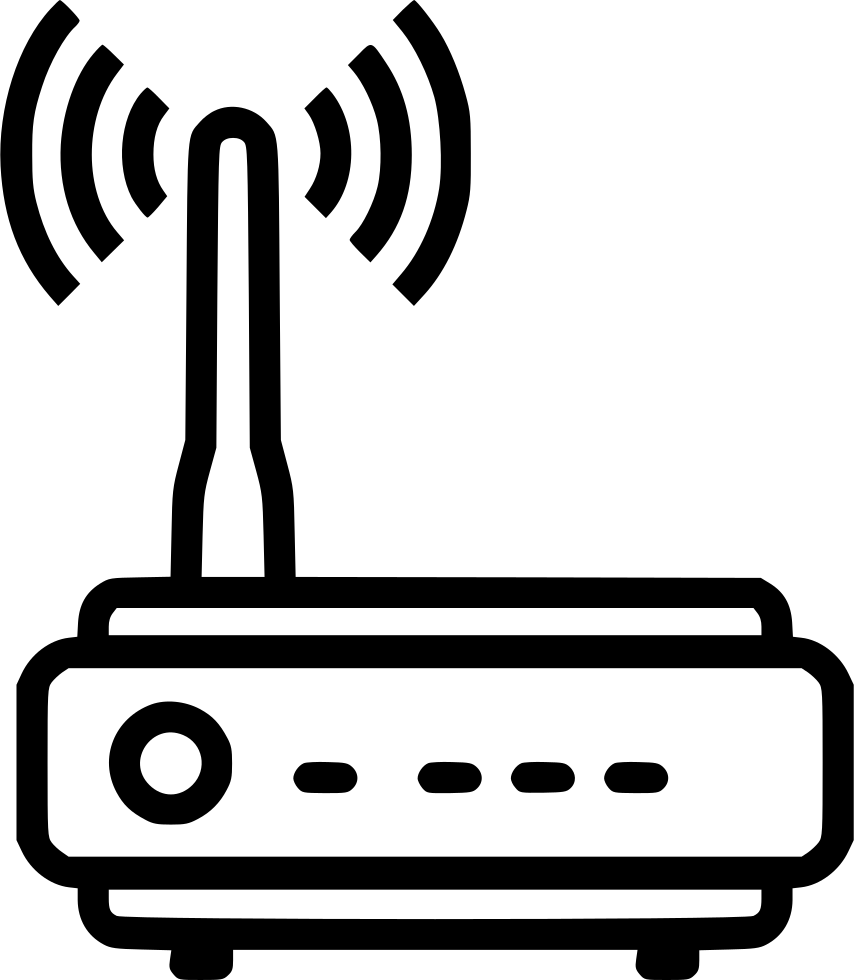
\includegraphics[width=1cm]{images/router.png}};
        \node[label={180:192.168.1.2}] at (-5,2) (b) {
\includegraphics[width=1cm]{images/computer.png}};
        \node[label=180:{192.168.1.3}] at (-6,1) (c) {
\includegraphics[width=1cm]{images/computer.png}};
        \node[label=180:{192.168.1.4}] at (-7,0) (d) {
\includegraphics[width=1cm]{images/computer.png}};
        \draw[dashed,very thick] (b) -- (a) (c) -- (a) (d) -- (a);
        \node[draw,thick,right,align=left] at (-6,-0.7) (packet) {\scriptsize Source: 192.168.1.4\\\scriptsize Destination: 208.80.153.224};
        \draw[thick,->] (packet) -- (-1.5,-0.7);
        \node[draw,thick,right,align=left] at (2,-0.7) (packet2) {\scriptsize Source: 172.217.15.100\\\scriptsize Destination: 208.80.153.224};
        \draw[thick,->] (1,-0.7) -- (packet2);
        \draw[dashed,very thick] (a) -- ++(5,0) node[above left] (cloud) {
\includegraphics[width=2cm]{images/cloud.png}};
        \node at (cloud) {Internet};
        \end{scope}
    \end{tikzpicture}
    \caption{The default gateway forwards packets from a LAN to a WAN.}
    \label{fig:gateway}
\end{figure}

\subsection{Autonomous Systems}

Once a packet is routed to a wide area network, such as the Internet, it needs to be sent to the network which contains the destination address. Typically, the first destination for a packet is a router belonging to an Internet Service Provider (ISP). For example, in the \texttt{traceroute} trace on page \pageref{code:traceroute}, the packet ends up at a router owned by Verizon, a popular ISP. This router belongs to an \emph{autonomous system} (AS) operated by Verizon. An autonomous system is simply a connection of routers on the Internet which are under some common administrative control, such as by an ISP.

Autonomous systems are managed globally using autonomous system numbers, or ASNs, which are similar to IP addresses. These numbers are allocated by the Internet Assigned Numbers Authority (IANA) to Regional Internet Registries (RIRs), which then assign the numbers to autonomous systems.

The routers in an autonomous system can forward packets to destinations within the same AS, but if a packet is destined for a network on another AS, it needs to be routed appropriately. This requires different ASs to communicate with one another. This can happen via \emph{peering}, in which two ASs mutually agree to carry traffic to one another free of charge, or via \emph{transit}, in which an AS charges a fee to carry traffic from other ASs.

When two ASs need to communicate with one another, they use the Border Gateway Protocol (BGP). This is the core routing protocol of the Internet, and is responsible for making decisions on how to get packets to a destination in the quickest way possible. 

\section{Network Security}\label{sec:network:security}

One of the most important issues with computer networks is security. The Internet is frequently used for transmitting confidential messages, facilitating financial transactions, and other applications where security is paramount. For this reason,there are protocols dedicated to ensuring that the Internet can be secure. The most common such protocol is Transport Layer Security (TLS), which is a successor to an older protocol called Secure Sockets Layer (SSL). TLS is implemented at the transport layer of a network. Web traffic which uses TLS/SSL security is sent using the HTTPS protocol at the application layer, rather than the unsecured HTTP protocol.

Another common network security application is a Virtual Private Network, or VPN. A VPN allows computers connected to different LANs to communicate over the Internet as if they belonged to the same LAN. This is often used by companies to allow employees to access private resources even when they are away from the office. Security is very important for a VPN, and it can be provided using TLS or other protocols.

The details of TLS are complicated, and we will not get into them here. Instead, we will cover what exactly security means in a network setting, and look at three goals of any secure network: privacy, authenticity, and reliability. Achieving these goals requires using tools from cryptography, which you may learn about in a future course.

\subsection{Privacy}

When two parties want to securely transmit a message, one of their most straightforward goals is privacy. The two parties do not want a third party to be able to lisen in on their communication.

Following a standard convention in cryptography, we will denote the two parties by Alice and Bob, and the adversarial third party by Carol. Alice is sending a message to Bob, and Carol wants to listen in. Since network signals travel over cables, Carol could listen in to the signal by physically tapping into a wire. Even more easily, on a wireless network, all signals are broadcast over the air and can be received by anyone who wants to listen.

In order to protect their messages from being read by Carol, Alice and Bob use an encryption algorithm. Alice and Bob have some shared key, and when Alice wants to send a message, she first uses her key to turn the plain text of the message into a cipher text. If the algorithm is secure, then the cipher text cannot be converted back to the plain text without knowledge of the key. This way, if Carol manages to read the message, she will only see nonsensical cipher text. Only Bob, who has the key, can produce the plain text.

A key issue here is how Alice and Bob come to have the same key. If Alice tells Bob her key over the network, then Carol could retrieve the key and use it to decrypt all future messages. This is a fundamental problem in cryptography called the key-sharing problem. It is solved using a technique called public key cryptography. In TLS, public key cryptography is implemented using either the RSA algorithm, or a more sophisticated method called elliptic curve cryptography (ECC). These algorithms allow Alice and Bob to generate shared keys which Carol cannot intercept.

\subsection{Authenticity}

Even if Carol cannot read messages sent between Alice and Bob, she can still do damage. One potential attack would be for Carol to impersonate Alice, by sending a message to Bob which says it comes from Alice. This is why TLS must also protect the authenticity of messages: if a message says it comes from Alice, Bob needs some way of verifying that this is actually the case.

The public key cryptography algorithms used for ensuring privacy can also provide authenticity. In these algorithms, every party on the network has a private key which is never shared with anyone. This private key is important for generating the shared keys used for encrypting messages. It can also be used to generate a ``digital signature,'' which could only be produced by someone in possession of the private key. As long as the private key has never been shared, a digital signature can provide a guarantee of authenticity.

\subsection{Integrity}

Finally, even if Carol cannot read messages or impersonate Alice or Bob, she could try to modify one of their messages. This is called a man-in-the-middle (MITM) attack, where Carol intercepts Alice's communications, edits them, and then forwards them to Bob with Alice's signature intact.

To protect against this, TLS uses a message authentication code (MAC) which is sent along with any message. This is a short code sent with the message, which depends on the shared key and on the message. If the algorithms are secure, then it should be nearly impossible to generate a MAC without knowledge of both the shared key and the message. When Bob receives the message along with the MAC, he verifies that the MAC is correct. If it is not, then he knows the message has been altered in transit and discards it.

\subsection{Security versus Trust}

An enormous amount of expertise, testing, and iteration has gone into making TLS secure. However, it is still relatively common to hear about security problems on the Internet. Where do these problems come from?

In this context, it is important to recognize a key difference between security and trust. Network security provided by TLS achieves the three goals outlined above: privacy, authenticity, and integrity. When Alice communicates with Bob, she can be sure that only Bob can read her messages, that messages she receives from Bob really come from Bob, and that the messages have not been altered in transit. However, \emph{TLS does not guarantee that Alice can trust Bob}.

There are many ways in which Bob could be unreliable. For example, Bob could be attempting to execute a phishing attack by impersonating someone else. TLS guarantees that Bob cannot truly impersonate \texttt{facebook.com}, but he could own \texttt{fcebook.com} and, using TLS security, provide a website that looks just like \texttt{facebook.com} and asks for your login credentials. If you provide them to \texttt{fcebook.com}, then Bob could read your password and log into your actual Facebook account.

Even if Bob is not malicious, he could be irresponsible. For example, if Bob runs an online vendor which collects credit card information to make payments, it is crucial that Bob takes appropriate security measures on his local network to protect that credit card information from becoming known to an attacker. TLS does not guarantee that Bob has taken the necessary precautions. Many of the most substantial security problems arise on the Internet when many customers have trusted a vendor like Bob with their personal details like credit card numbers, and Bob suffers a data breach, putting this data into the wrong hands.

Network security is an evolving field as companies and governments work to protect against these sorts of vulnerabilities. There are many opportunities for employment in this area, as organizations increasingly need to rely on dedicated security professionals in order to keep their data and their clients' data safe.
	\pagebreak
	\chapter{Control Structures}

So far, we have seen programs in which each statement is executed in order, one by one. Today we will learn about \emph{conditionals}, which allow us to execute statements depending on certain conditions. This is our first exposure to the idea of \emph{control flow}, which refers to the order (or sequence) in which statements of a program are executed.

In this chapter, we will first learn about \ic{if} statements, which allow us to write programs based on conditions. Then we will learn about \ic{else} statements. We will combine these \ic{if} and \ic{else} statements into more complex nested structures, and then finally learn about \ic{else if} statements. Lastly, this chapter ends with a list a common mistakes to avoid when writing conditionals.

\section{The \ic{if} statement}

\begin{definition}
An \emph{if statement} is a \emph{conditional statement} that consists of the reserved keyword \ic{if}, followed by a boolean expression enclosed in parentheses, followed by a statement typically enclosed in curly braces. If the boolean expression (or \emph{condition}) evaluates to true, the statement is executed. Otherwise, it is skipped.
\end{definition}

An \ic{if} statement allows us to write programs that decide whether to execute a particular statement, based on a boolean expression which we call the \emph{condition}. Below is an example of a simple \ic{if} statement:

\begin{code}
if (count > 20) {
    System.out.println("Count exceeded");
}
\end{code}

\noindent The condition in this example is \ic{count > 20}. It is a boolean expression that evaluates to either true or false. That is, \ic{count} is either greater than \ic{20} or not. If it is, ``Count exceeded" is printed. Otherwise, the \ic{println} statement is skipped. 

\begin{example}
What does the following piece of code print if \ic{x} is 101? What about if \ic{x} is 200? What about if \ic{x} is 8?

\begin{code}
if (x > 100) {
    System.out.println("Big number!");
} 
System.out.println("Hi there");
if (x % 2 == 0) { // checks if a number is even*
    System.out.println("Even number!");
}
\end{code}

* Recall that the modulo operator (\%) computes the remainder of some number. By checking if the remainder of some number when divided by 2 is 0, we are checking if that number is even. \\

\emph{Answer}: If \ic{x} is 101, the first boolean expression will evaluate to true, so the program will print ``Big number!" Then the program will print ``Hi there" regardless of any condition. Finally, since 101 is not even, the program will not print ``Even number!"

Using the same reasoning to trace the execution with \ic{x} as 200, the following statements will be printed: ``Big number! Hi there! Even number!"

When \ic{x} is 8, the output is ``Hi there! Even number!"
\end{example}

\begin{example}
How would you fill in the boolean expression below to take the absolute value of an integer \ic{x}? (Hint: to take an absolute value of a negative number, you must negate it).

\begin{code}
if (/* Insert boolean expression here */) {
    x = -x;
} 
\end{code}

\emph{Answer}: Insert the boolean expression x $<$ 0.
\end{example}

\section{The \ic{else} statement}
Sometimes we want to do one thing if a condition is true and another thing if that condition is false. We can add an \ic{else} clause to an \ic{if} statement to handle this kind of situation. Below is an example of a simple \ic{if-else} statement:

\begin{code}
if (price > 20) {
    System.out.println("Too expensive");
} else {
    System.out.println("Affordable");
}
\end{code}

\noindent This example prints either ``Too expensive" or ``Affordable", depending on whether \ic{price} is greater than 20. Only one or the other is ever executed, never both. This is because boolean conditions only evaluate to either true or false.

Note that it is not possible to have an \ic{else} statement without having a corresponding \ic{if} statement. Any \ic{else} statement must be attached to a preceding \ic{if} statement. 

\begin{example}
What does the following piece of code do?

\begin{code}
if (balance <= 0) {
    System.out.println("Unable to withdraw");
} else {
    System.out.println("Withdraw successful");
}
\end{code}

\emph{Answer}: It prints ``Unable to withdraw" if balance is 0 or lower. Otherwise, it prints ``Withdraw successful".
\end{example}

\begin{example}
Rewrite the code below using an \ic{else} statement.

\begin{code}
if (rating >= 4) {
    System.out.println("Would recommend");
} if (rating < 4) {
    System.out.println("Would not recommend")
}
\end{code}

\emph{Answer}: Since the second boolean expression is the negation of the first boolean expression, we can replace the second \ic{if} statement with an \ic{else}.
\begin{code}
if (rating >= 4) {
    System.out.println("Would recommend");
} else {
    System.out.println("Would not recommend")
}
\end{code}
\end{example}

\begin{example}
Does the following code compile?

\begin{code}
else {
    System.out.println("Hello");
}
\end{code}

\emph{Answer}: No, since an \ic{else} statement must have a corresponding \ic{if} statement.
\end{example}

\begin{example}
Does the following code compile?

\begin{code}
if (duration > 60) {
    System.out.println("Sorry, that's too long");
} else {
    System.out.println("I can fit that in my schedule");
} else {
    System.out.println("Let me know when you are free")
}
\end{code}

\emph{Answer}: No, since an \ic{if} statement may only have at most 1 corresponding \ic{else} statement.
\end{example}

\section{Nested conditionals}
It is possible to combine \ic{if} and \ic{else} statements in more interesting ways, by nesting them. Consider the following example:

\begin{code}
if (x < y) {
    System.out.println("x is less than y");
} else {
    if (x > y) {
        System.out.println("x is greater than y");
    } else {
        System.out.println("x is equal to y");
    }
}
\end{code}

\noindent This example correctly prints out the relationship between two integer variables \ic{x} and \ic{y} using nested conditionals. No matter what the values of \ic{x} and \ic{y} are, only a single statement will be printed. 

\begin{example}
Fill in each blank below with \ic{if} or \ic{else} to describe a person's height.

\begin{code}
/*__________*/ (height < 60) {
    System.out.println("Relatively short")
} /*__________*/ {
    /*__________*/ (height > 72) {
        System.out.println("Relatively tall");
    } /*__________*/ {
        System.out.println("Pretty average");
    }
}
\end{code}

\emph{Answer}: The four blanks should contain \ic{if}, \ic{else}, \ic{if}, and \ic{else}, in that order.
\end{example}

\begin{example}
Given integer variables \ic{a} and \ic{b} and the following piece of code, what value gets stored in variable \ic{c}?

\begin{code}
int c;
if (a > b) {
    c = a;
} else {
    if (b > a) {
        c = b;
    } else {
        c = 0;
    }
}
\end{code}

\emph{Answer}: The larger of the two variables, \ic{a} and \ic{b}, gets stored in \ic{c}. If \ic{a} and \ic{b} are equal, 0 gets stored in \ic{c}.
\end{example}

\begin{example}
Imagine that the following program represents the person's reaction to different types of food. Given a pizza (\ic{green} = false, \ic{bitter} = false, \ic{warm} = true, \ic{cheesy} = true), how will this person respond? What about when given a kiwi (\ic{green} = true, \ic{bitter} = false, \ic{warm} = false, \ic{cheesy} = false)? What about a strawberry (\ic{green} = false, \ic{bitter} = false, \ic{warm} = false, \ic{cheesy} = false)?

\begin{code}
if (green || bitter) {
    System.out.println("No thank you");
} else {
    if (warm && cheesy) {
        System.out.println("Yum, yes please!");
    } else {
        System.out.println("Thank you, I'll take some");
    }
}
\end{code}
\emph{Answer}: The person reponds ``Yum, yes please!" to pizza, ``No thank you" to kiwi, and ``Thank you, I'll take some" to strawberry.
\end{example}

\section{The \ic{else if} statement}
Nested conditionals are useful in many applications, but they can start feeling clunky as the nesting becomes deep. For example, consider the following piece of code:

\begin{code}
if (grade > 90) {
    System.out.println("You earned an A");
} else {
    if (grade > 80) {
        System.out.println("You earned a B");
    } else {
        if (grade > 70) {
            System.out.println("You earned a C");
        } else {
            if (grade > 60) {
                System.out.println("You earned a D");
            } else {
                System.out.println("You earned an F");
            }
        }
    }
}
\end{code}

\noindent To avoid having such deeply nested conditionals, we introduce the \ic{else if} clause. Using \ic{else if} statements, we can rewrite the above program as:

\begin{code}
if (grade > 90) {
    System.out.println("You earned an A");
} else if (grade > 80) {
    System.out.println("You earned a B");
} else if (grade > 70) {
    System.out.println("You earned a C");
} else if (grade > 60) {
    System.out.println("You earned a D");
} else {
    System.out.println("You earned an F");
}
\end{code}

You can imagine an \ic{else if} statement as shorthand for an \ic{if} nested inside an \ic{else}. For example, the following snippets of code behave identically (for any boolean expressions A and B):

\begin{code}
// Version 1 (using nested conditionals)
if (A) {
    System.out.println("A");
} else {
    if (B) {
        System.out.println("B");
    } else {
        System.out.println("C");
    }
}

// Version 2 (equivalent, using else if)
if (A) {
    System.out.println("A");
} else if (B) {
    System.out.println("B");
} else {
    System.out.println("C");
}
\end{code}

It is very common to see a conditional block of code that consists of 1 \ic{if} statement, 0 or more \ic{else if} statements, and 1 \ic{else} statements. In these cases, recall that only one of these statements will ever execute.

\begin{example}
Imagine \ic{A} and \ic{B} are boolean expressions. If both of them evaluate to true, what does the following code print out?

\begin{code}
if (A) {
    System.out.println("apple");
} else if (B) {
    System.out.println("banana");
} else {
    System.out.println("carrot");
} 
System.out.println("dragonfruit");
\end{code}

\emph{Answer}: The code will print ``apple" and then ``dragonfruit". Notice that ``banana" does not get printed even though \ic{B} is true since the entire \ic{if}, \ic{else if}, \ic{else} chain will only ever print one of ``apple", ``banana", and ``carrot". 
\end{example}

\begin{example}
Imagine \ic{X}, \ic{Y}, and \ic{Z} are boolean expressions. If \ic{X} evaluates to true, but \ic{Y} and \ic{Z} evaluate to false, what does the following code print out?

\begin{code}
if (X && Y) {
    System.out.println("xylophone");
} else if (!Z) {
    System.out.println("zoo");
}
\end{code}

\emph{Answer}: This code will print ``zoo". Notice that the boolean expressions used with \ic{if} statements can be complex and contain boolean operators such as \ic{\&\&} and \ic{||} and \ic{!}, as long as the expression evaluates to a true or false.
\end{example}

\section{Curly braces}
So far, we have been using curly braces to enclose each of our \ic{if}, \ic{else if}, and \ic{else} statements. These curly braces can be omitted if there is only a single statement. For example, in the snippet of code below, the first set of curly braces can be omitted, while the second cannot.

\begin{code}
if (guess == answer) {
    System.out.println("You guessed correctly!");
} else {
    System.out.println("Sorry, you guessed incorrectly.");
    System.out.println("The answer was " + answer);
} 
\end{code}

\noindent If all the curly braces were left out (as in the code below), the program would first either print ``You guessed correctly!" or ``Sorry, you guessed incorrectly.", but then also print ``The answer was ..." in all cases, regardless of the condition.

\begin{code}
if (guess == answer)
    System.out.println("You guessed correctly!");
else
    System.out.println("Sorry, you guessed incorrectly.");
    System.out.println("The answer was " + answer); 
    // ^^^ Careful! This is not part of the else clause!
\end{code}

Here it is important to note that whitespace and indentation are ignored by Java. Indentation has no effect on the behavior of a program. Proper indentation is extremely important for human readability. When used incorrectly, however, misleading indentation can result in unexpected behavior.

\begin{example}
Does the following code compile and print the larger of two integers \ic{a} and \ic{b} correctly?

\begin{code}
if (a > b)      System.out.println("a");
else {
System.out.println("b");
}
\end{code}

\emph{Answer}: Yes! Even though the whitespacing and indentation look funny, this piece of code compiles correctly.
\end{example}

\section{Common mistakes}
When writing conditional structures, beware of the following common  mistakes:

\subsection{Forgetting parentheses}
In Java, the parentheses surrounding the boolean expression in conditional structures are required. For example, the following code will not compile.
\begin{code}
if count > 10
    System.out.println("So many!");
\end{code}

\subsection{Accidental semi-colons}
Accidentally semi-colons immediately after the parentheses around the boolean expression in an \ic{if} statement is one of the trickiest mistakes to detect. The following code compiles, but it behaves unexpectedly. 
\begin{code}
if (count > 10);
    System.out.println("So many!");
\end{code}

\noindent The code above is misleading because it is identical to the following:
\begin{code}
if (count > 10) {
    ;
}
System.out.println("So many!");
\end{code}

\noindent The accidental semi-colon is treated as a single, ``do-nothing" statement.

\subsection{Missing curly braces}
As mentioned before, indentation helps make code more readable to humans, but it can also make code more confusing if used incorrectly. It is a common mistake to accidentally forget curly braces.

\begin{code}
if (leaves = 4) {
    System.out.println("You found a four-leaf clover, how lucky!");
} else
    System.out.println("Sorry, not a four-leaf clover.");
    System.out.println("Keep looking!");
\end{code}

\noindent This code above is misleading because it prints ``Keep looking!" regardless of whether a four-leaf clover was found. The writer of this program probably meant to add curly braces around the \ic{else} clause.

\subsection{\ic{else} without an \ic{if}}

Although the following example looks fine at first glance, it does not compile. This is because the \ic{else} clause is nested \emph{inside} the \ic{if} statement instead of acting as an \emph{alternative} option to the \ic{if} statement.

\begin{code}
if (chanceOfRain > 50) {
    System.out.println("Bring an umbrella!");
    else {
        System.out.println("Hm, I don't think it will rain today.")
    }
}
\end{code}

\noindent To fix the code above, move the \ic{else} statement \emph{outside} of the \ic{if} as below:

\begin{code}
if (chanceOfRain > 50) {
    System.out.println("Bring an umbrella!");
} else {
    System.out.println("Hm, I don't think it will rain today.")
}
\end{code}

\subsection{Assignment v.s. equality operator}
It is very easy to mix up the assignment operator (the single equals sign \ic{=}) with the equality operator (the double equals sign \ic{==}). The following code is incorrect and results in a compilation error:

\begin{code}
if (temperature = 0) {
    System.out.println("It's freezing!");
}
\end{code}

\noindent The assignment operator cannot be used here because conditional structures require a boolean expression (i.e. something that evaluates to either true or false). 

\exercisesection

\begin{exercise}
What output is produced by the following code fragment?

\begin{code}
int num = 87;
int max = 25;
if (num >= max*2)
    System.out.println("apple");
    System.out.println("orange");
System.out.println("pear");
\end{code}

TODO: modify this exercise, or make sure we can reference the Java Foundations textbook
\end{exercise}

\begin{exercise}
What output is produced by the following code fragment?

\begin{code}
int limit = 100;
int num1 = 15;
int num2 = 40;
if (limit <= limit) {
    if (num1 == num2)
        System.out.println ("lemon");
    System.out.println ("lime");
}
System.out.println ("grape");
\end{code}

TODO: modify this exercise, or make sure we can reference the Java Foundations textbook
\end{exercise}


\begin{exercise}
Given a day of the week encoded as 0=Sun, 1=Mon, 2=Tue, ...6=Sat, and a boolean indicating if we are on vacation, we need to decide when to set our alarm clock to ring. We want to wake up at ``7:00" on weekdays and ``10:00" on weekends. However, if we are on vacation, it should be ``10:00" on weekdays" and ``off" on weekends. Imagine you are given an integer variable \ic{day} and a boolean variable \ic{vacation}. Write a program that prints out the appropriate alarm time.

TODO: modify this exercise, or make sure we can reference codingbat.com
\end{exercise}

\begin{exercise}
Your cell phone rings. Normally you answer, except in the morning you only answer if it is your mom calling. In all cases, if you are asleep, you do not answer. Given three booleans, \ic{isMorning}, \ic{isMom}, and \ic{isAsleep}, write a program that correctly prints out whether or not you will pick up your phone (``Answer" or ``Do not answer"). 

For example, if \ic{isMorning}, \ic{isMom}, and \ic{isAsleep} are all false, print ``Answer". 

TODO: modify this exercise, or make sure we can reference codingbat.com
\end{exercise}

\begin{exercise}
You have a lottery ticket with a 3-digit number. If your ticket has the number 777, you win \$100. If your ticket has a number with the same 3 digits (like 222, for example), then you win \$10. Otherwise, you don't earn any money. Given three integers, \ic{a}, \ic{b}, and \ic{c}, that represent the digits of your lottery ticket, write a program that prints out how much money you earn.

For example, if your ticket number is 123 (\ic{a} = 1, \ic{b} = 2, \ic{c} = 3), print ``\$0". 

TODO: modify this exercise, or make sure we can reference codingbat.com
\end{exercise}

\referencessection

Computer Science: An Interdisciplinary Approach, Robert Sedgewick and Kevin Wayne.

Lewis, John, Peter DePasquale, and Joseph Chase. Java Foundations: Introduction to Program Design and Data Structures. Addison-Wesley Publishing Company, 2010.

Programming exercises from codingbat.com
	\pagebreak
	\chapter{Business Software}

\section{Introduction}

This lecture will go over three primary types of business productivity software most businesses use on a daily basis: 
\begin{enumerate}
	\item Word processing software: for typing and formatting text and images on a page (such as essays and reports) 
	\item Presentation software: for creating slides with information and graphics (such as for meetings and briefings)
	\item Spreadsheet software: for storing data, doing computations, and making graphs
\end{enumerate}

\section{Word Processing}

Word processing software is used for creating, editing, and formatting documents. Many tech companies have their own version of word processing software. A few more familiar examples include
\begin{itemize}
	\item Microsoft Word
	\item Apple Pages
	\item Google Docs
\end{itemize}

Beyond providing an interface to type the words of your report or essay into, word processors allow a variety of styling and formatting options to customize the document to look the way you like it. For example, all of the word processors above support
\begin{itemize}
	\item Automatic page numbering
	\item Adjustable margins
	\item Varieties of text size, text font, text color
	\item Addition of images and captions, along with image formatting
	\item Addition of tables and lists 
	\item Spelling and grammar checking
\end{itemize}

% Pop in  a picture

\section{Spreadsheets}

Spreadhseet software is used for dealing with data. A few examples of spreadsheet software include
\begin{itemize}
	\item Microsoft Excel
	\item Apple Numbers
	\item Google Sheets
\end{itemize}

Beyond providing a grid in which you can type numbers, spreadsheet software facilitate a variety of operations on the data. styling. A few key features supported by most spreadsheet applications include
\begin{itemize}
	\item Statistical analysis
	\item Sorting
	\item Creating charts and graphs
	\item Formatting (e.g. adding color, borders, etc.)
\end{itemize}

% maybe some activities here about what you would do with given data? 
% probably want to add pictures to illustrate each of the operations above 

\section{Presentations}

Presentation software is used for presenting data and graphics to an audience. Some common examples include
\begin{itemize}
	\item Microsoft Powerpoint
	\item Apple Keynote
	\item Google Slides
\end{itemize}

All of these software give the user a series of "slides" that can be clicked through during a presentation. It allows the presenter to focus the audience's attention on a single point at a time. The slides are not meant to contain all the information that the presenter wants to get across. Instead, the slides only mention the key takeaways, and the presenter should verbally fill in the details. For that reason, slides often consist of just a few bullet points and an image. Of course, there are a variety of creative ways to present - this is just the most common format!

A few particularly important features offered by almost all presentation software include
\begin{itemize}
	\item Automatic styling (color schemes, layouts, etc) 
	\item Add images and videos
	\item Slide transitions 
	\item Animations (e.g. showing one line of text on a slide at a time) 
\end{itemize}

\section{Project} 


	\pagebreak
	\chapter{Methods}

% Abstraction, modularity, code-reuse, syntax, arguments and calling

Sometimes it is useful to abstract certain computations into methods.
In this chapter, we will be looking at how and why we can use methods to
achieve more concise and easily-maintainable code.

We will first look at some code that does not use methods and identify some
problems with this code. We will then, in Section \ref{sec:methods},
introduce what a method is, including how to define and use them.
In Sections \ref{sec:abstraction} and \ref{sec:modularity}, we will
then talk about how we can use methods to improve the problems that
we noticed with our code. In particular, in Section \ref{sec:abstraction},
we talk about how methods allow us to abstract some of our code to get
more concise and maintainable code, and in Section \ref{sec:modularity},
we talk about how methods allow us to divide our code up into chunks
that we can consider in isolation, allowing us to manage and maintain
our code more easily.

Let us consider the following problem:

We have a class of nine students, split up into three groups of three.
For each group, we want to report the maximum score for each group.
%as well as the maximum score for the students overall.
We will use the variable names \ic{group1s1}, \ic{group1s2}, and \ic{group1s3}
to refer to the three scores achieved by the students in Group 1, and we will use
a similar naming convention for the variable names for the scores achieved by
students in Group 2 and Group 3.

The following snippet of code computes the maximum score in Group 1, storing
the result in \ic{group1Max}.
\begin{code}
int group1Max = group1s1;
if (group1s2 > group1Max) {
  group1Max = group1s2; 
}
if (group1s3 > group1Max) {
  group1Max = group1s3; 
}
\end{code}

If we now wish to extend this to compute the maximum score for each group,
we can copy the code and rename the variables to achieve the following
code:
\begin{code}
int group1Max = group1s1;
if (group1s2 > group1Max) {
  group1Max = group1s2; 
}
if (group1s3 > group1Max) {
  group1Max = group1s3; 
}

int group2Max = group2s1;
if (group2s2 > group1Max) {
  group2Max = group2s2; 
}
if (group2s3 > group2Max) {
  group2Max = group2s3; 
}

int group3Max = group3s1;
if (group3s2 > group3Max) {
  group3Max = group3s2; 
}
if (group3s3 > group3Max) {
  group3Max = group3s3; 
}
\end{code}

\noindent There are a couple of things about the process of getting this resulting code
that aren't particularly ideal.
The first is that it is very easy to make a mistake when copying the code and renaming
the variables. For example, we might have missed renaming \ic{group1Max} to \ic{group3Max}
in the computation of the maximum score for Group 3, leading us to compute an incorrect maximum
value in some cases.

The second issue is that there is a lot of redundancy.
If we look at the code, we can notice that there seem to be a lot of redundant parts
across the code for the three different groups.
If we had ended up with the wrong computation initially and needed to fix it
later, then we would have to make sure we fixed it everywhere, leading to repeated work and the
possibility that we didn't fix one of the copies. For example, if we initially started out with
\ic{group1s3 < group1Max} instead of \ic{group1s3 > group1Max}, and then copied and renamed variables
to compute the maximum scores for the other groups, we would end up with the code below:

\begin{code}
int group1Max = group1s1;
if (group1s2 > group1Max) {
  group1Max = group1s2;
}
if (group1s3 < group1Max) {
  group1Max = group1s3;
}

int group2Max = group2s1;
if (group2s2 > group1Max) {
  group2Max = group2s2;
}
if (group2s3 < group2Max) {
  group2Max = group2s3;
}

int group3Max = group3s1;
if (group3s2 > group3Max) {
  group3Max = group3s2;
}
if (group3s3 < group3Max) {
  group3Max = group3s3;
}
\end{code}

To fix our code, we would not only have to replace \ic{group1s3 < group1Max} with
\ic{group1s3 > group1Max}, but we would also need to replace \ic{group2s3 < group2Max} with
\ic{group2s3 > group2Max} and \ic{group3s3 < group3Max} with \ic{group3s3 < group3Max}.

\section{Methods}\label{sec:methods}
In Java, we can use abstractions in our code in the form of \emph{methods}.
Methods contain bits of code that may compute things using \emph{arguments}
that are passed into the method.

An example of the syntax for a \emph{method definition} is given below:
\begin{code}
public bool negate(bool arg) {
  return !arg; // method body
}
\end{code}
We can identify the different components of the method definition:
\begin{itemize}
\item  The \emph{access modifier} of the method is \ic{public},
\item the \ic{bool} before \ic{negate} gives the \emph{return type} of the method
\item \ic{negate} is the \emph{name of the method},
\item \ic{arg} is the \emph{name of the first argument/parameter} of the method,
\item the \ic{bool} before \ic{arg} it is the \emph{type} of the \ic{arg} parameter,
\item and the code between the curly braces is the method \emph{body}.
\end{itemize}
Inside the method body, there is code that may use the arguments of the method.
In the example above, the body only consists of the \ic{return} statement.
The \ic{return} statement is followed by something of the return type of the method.
This expression, after being evaluated, gives the \emph{return value} of the method.
As soon as a \ic{return} statement is encountered, a method finishes its execution.
\emph{Access modifiers} will be described later on when we talk about Classes,
but note that if an access modifier is omitted, it the method has the \emph{default} modifier.

Other important terms to note are as follows:
The \emph{parameter list} of a method consists of the types of its parameters in the
order they are given in the method definition.
For the above method, it is simply \ic{bool}.
The \emph{method signature} consists of the method name and parameter list.
For the above method, it is \ic{negate(bool)}.
A method is identified by its method signature.

\begin{example}
Consider the following method:
\begin{code}
int squareSum(int arg0, int arg1) {
  int res = arg0 + arg1;
  return res * res;
}
\end{code}
Give the following for the method:
\begin{itemize}
\item Access modifier
\item Return type
\item Arguments
\item Method signature
\end{itemize}

\noindent \emph{Answer}: 
\begin{itemize}
\item Access modifier: default
\item Return type: \ic{int}
\item Arguments: \ic{arg0}, \ic{arg1}
\item Method signature: \ic{squareSum(int, int)}
\end{itemize}
\end{example}

\begin{example}
Consider the following method:
\begin{code}
private void mystery (int age, String name) {
  if (age >= 18) {
    System.out.println(name);
  }
}
\end{code} 
Give the following for the method:
\begin{itemize}
\item Access modifier
\item Return type
\item Name
\item Parameter list
\end{itemize}

\noindent \emph{Answer:}
\begin{itemize}
\item Access modifier: \ic{private}
\item Return type: \ic{void}
\item Name: \ic{mystery}
\item Parameter list: \ic{int, String}
\end{itemize}

\end{example}

We may \emph{call} or \emph{invoke} the above \ic{negate} method from elsewhere in the code by,
for example, using \ic{negate(true)} if we want to call \ic{negate} with argument
\ic{true}.
We must specify the name of the method that we wish to call, followed by the arguments
that we wish to call it on, separated by commas if there are more than one.
The arguments provided in the call must correspond to the types of the arguments
specified in the method definition: if the method definition has the type \ic{bool}
for its first argument, then the first argument supplied in the call should also be
of type \ic{bool}, and if the definition has the type \ic{int} for its second argument,
then the first argument in the call should also be of type \ic{int}, and so on.
A method invocation evaluates to the return value it computes, where this
computation happens with the actual arguments
given in the call substituted for the arguments specified in the definition, so in
this case, the invocation \ic{id(true)} evaluates to \ic{false}.
A method invocation has the same type as its return type, which in this case, is \ic{bool}.

So, for example, we can do something like in following code snippet:
\begin{code}
  bool f = negate(true);
  bool t = negate(negate(true));
\end{code}
After executing the above code, the variable \ic{f} contains the value \ic{false}
and the variable \ic{t} contains the value \ic{true}.

Note that we can also have methods that do not return anything. Such
methods have \ic{void} return types. They may contain a \ic{return}
statement with no expression following \ic{return}.
Calls to these methods cannot be used inside of other expressions.
Two examples of methods with \ic{void} return types are below:
\begin{code}
public void printSum(double a, double b) {
  System.out.println(a + b);
}
\end{code}

\begin{code}
public void printBigger(double a, double b) {
  if (a > b) {
    System.out.println(a);
    return;
  }
  System.out.println(b);
}
\end{code}
Note that the latter example only ever prints the value of either \ic{a} or \ic{b} but
never both because
the \ic{return} statement finishes the execution of the method.

Some methods also do not take any arguments at all. One such example is below:
\begin{code}
public int constantOne() {
  return 1;
}
\end{code}
\noindent This method can be called using \ic{constantOne()}.

\begin{example}
What value does \ic{res} have after the following code snippet is executed?
\begin{code}
int res = constantOne() + constantOne();
\end{code}
\emph{Answer}: The value of \ic{res} is 2.
\end{example}.

Note that for every method that does not have a \ic{void} return type,
for every possible control-flow path through the method body,
there must be a \ic{return} statement that is eventually reached.
For example, the following method does not meet this requirement
because when \ic{arg} is \ic{false}, the \ic{return} statement is not
reached:
\begin{code}
public int twoIfTrue(bool arg) {
  if (arg) {
    return 2;
  }
}
\end{code}

\begin{example}
Consider the following method:
\begin{code}
public void mystery (bool arg0, int arg1) {
  if (arg0) {
    return -1 * arg1;
  }
  return arg0;
}
\end{code}

\noindent What do each of the following evaluate to?
\begin{itemize}
\item \ic{mystery(true, -2)}
\item \ic{mystery(true, 0)}
\item \ic{mystery(true, 4)}
\item \ic{mystery(false, -2)}
\item \ic{mystery(false, 0)}
\item \ic{mystery(false, 4)}
\end{itemize}

\noindent \emph{Answer:}
\begin{itemize}
\item \ic{mystery(true, -2)} evaluates to 2
\item \ic{mystery(true, 0)} evaluates to 0
\item \ic{mystery(true, 4)} evaluates to $-4$
\item \ic{mystery(false, -2)} evaluates to $-2$
\item \ic{mystery(false, 0)} evalutes to 0
\item \ic{mystery(false, 4)} evalutates to 4
\end{itemize}

\noindent What does the method do?

\noindent \emph{Answer:} It negates its second argument
\ic{arg1} whenever its first argument \ic{arg0} is
\ic{true} and otherwise just returns its second argument
\ic{arg1}.
\end{example}

\begin{example}
How many methods can be called by the following method?
What do you think each of their return types and parameter lists are?

\begin{code}
public void sayHello(int times, String name, String day) {
  if (shouldStop(times))
    return;
  String hello = getHelloStr(name, day);
  System.out.print.ln(hello);
  sayHello(times - 1, name, day);
}
\end{code}
\noindent \emph{Answer:}
Three methods can be called: \ic{shouldStop}, \ic{getHelloStr} and \ic{sayHello}.

The return type of \ic{shouldStop} is \ic{bool}, and it has parameter list \ic{int}.
The return type of \ic{getHelloStr} is \ic{String}, and it has parameter list \ic{String, String}.
The return type of \ic{sayHello} is \ic{void}, and it has parameter list \ic{int, String, String}.
\end{example}

\begin{example}
Write a method with signature \ic{printInOrder(int, int, int)} that takes
three \ic{int}s \ic{a}, \ic{b}, and \ic{c} as arguments and prints them out,
one per line, in increasing order. E.g. \ic{printInOrder(5, 9, 7)} should output the following:
\begin{code}
5
7
9
\end{code}

\noindent \emph{Answer:}
A possible solution is the following:
\begin{code}
public void printInOrder(int a, int b, int c) {
  int smallest = a;
  int middle = b;
  int biggest = c;
  if (smallest > middle) {
    int tmp = smallest;
    smallest = middle;
    middle = tmp;
  }
  if (smallest > biggest) {
    int tmp = smallest;
    smallest = biggest;
    biggest = tmp;
  }
  if (middle > biggest) {
    int tmp = middle;
    middle = biggest;
    biggest = tmp;
  }
  System.out.println(smallest);
  System.out.println(middle);
  System.out.println(biggest);
}
\end{code}
\end{example}

\subsection{Overloading}
As mentioned above, methods are identified by their signature, not just their names.
Because of this, we can actually have methods with the same name (in the same
Class) as long as they have different parameter lists.

For example, we can have the following two methods because
one has signature \ic{printBigger(double, double)} and the other
has signature \ic{printBigger(int, int)}:
\begin{code}
public void printBigger(double a, double b) {
  if (a > b) {
    System.out.println(a);
    return;
  }
  System.out.println(b);
}
public void printBigger(int a, int b) {
  if (a > b) {
    System.out.println(a);
    return;
  }
  System.out.println(b);
}
\end{code}
In this case, we say that the \ic{printBigger} method is \emph{overloaded}.

However, we cannot have the following two methods because they both have the
same signature \ic{twoIfTrue(bool)}:
\begin{code}
public int twoIfTrue(bool arg) {
  if (arg) {
    return 2;
  }
}
public double twoIfTrue(bool arg) {
  if (arg) {
    return 2.0;
  }
}
\end{code}

\begin{example}
Consider the following two methods that we have seen in previous
examples:
\begin{code}
private void mystery (int age, String name) {
  if (age >= 18) {
    System.out.println(name);
  }
}
public void mystery (bool arg0, int arg1) {
  if (arg0) {
    return -1 * arg1;
  }
  return arg0;
}
\end{code}
Are we allowed to have both of these methods together (in the same Class)?
Why or why not?

\noindent \emph{Answer:}
We are allowed to have both of these methods together because they have
different signatures. One has signature \ic{mystery(int, String)}
and the other has signature \ic{mystery(bool, int)}.
\end{example}

\begin{example}
Which of the following are valid overloadings?

\noindent A:
\begin{code}
public int absValue(int x) {
  if (x < 0) {
    return x * -1;
  }
  return x;
}
public double absValue(int x) {
  if (x < 0) {
    return 0.0 - x;
  }
  return x - 0.0;
}
\end{code}

\noindent B:
\begin{code}
public int absValue(int x) {
  if (x < 0) {
    return x * -1;
  }
  return x;
}
public double absValue(double x) {
  if (x < 0) {
    x = 0.0 - x;
  }
  return x;
}
\end{code}

\noindent C:
\begin{code}
public int absValue(int x) {
  if (x < 0) {
    return x * -1;
  }
  return x;
}
public int absValueX(int x) {
  if (x < 0) {
    return x * -1;
  }
  return x;
}
\end{code}

\noindent \emph{Answer:}
\begin{itemize}
\item A is not a valid overloading because both methods have the same signature.
\item B is a valid overloading because both methods have different signatures.
\item C is valid code, but this is not a valid overloading. It is not overloading at all because the methods have different names.
\end{itemize}
\end{example}

\subsection{Methods Summary}
In summary, every method definition has the following:
\begin{itemize}
\item An access modifier (if not explicitly stated, this will be the \emph{default} modifier)
\item A return type (possibly \ic{void})
\item A name
\item A (possibly empty) list of parameter types and names that can be passed to the method when it is called
\item A body
\item A return statement reached on every control path in the body, where each \ic{return} is followed by an
expression of the method's return type (unless the return type is \ic{void})
\end{itemize}
Each method is identified by its signature, so you may have methods with the same name but different parameter lists.

\section{Abstraction}\label{sec:abstraction}
Let us now return to our problem of finding the maximum scores for each
of the three groups.
The code for each of the three groups, though similar, have different variable names;
however, this is the only way in which they are different.
The process of distilling the similarity among different pieces of code is
the process of \emph{abstraction}.
In this case, we would like to \emph{abstract} away the details of
each copy to achieve a piece of code that describes all of their behavior.

After abstracting away the variable names, the code for each group is such that,
if we use the appropriate variable names for the students in the group
instead of \ic{x}, \ic{y}, and \ic{z}, that the following code snippet
would describe all of the three different operations, with
\ic{max} storing the desired result:
\begin{code}
int max = x;
if (y > max) {
  max = y; 
}
if (z > max) {
  max = z;
}
\end{code}
We can wrap this code snippet up in a method definition
that returns the value we care about:
\begin{code}
public int max3(int x, int y, int z) {
  int max = x;
  if (y > max) {
    max = y;
  }
  if (z > max) {
    max = z;
  }
  return max;
}
\end{code}

If we use this method in place of the redundant code,
our original code that compute the maximum scores for each of the three
groups then becomes as follows:
\begin{code}
int group1Max = max3(group1s1, group1s2, group1s3);
int group2Max = max3(group2s1, group2s2, group2s3);
int group3Max = max3(group3s1, group3s2, group3s3);
\end{code}
This resulting code is much more concise and is an example
of \emph{code reuse}, where the same exact code
(i.e. the code inside the body of \ic{max3}) is being reused
in several places. This code is also perhaps easier to understand
if you know that \ic{max3} simply calculates the maximum
of its three arguments. In the original code, after
going through the code for one of the groups
and realizing that it computes a maximum, you
would have to go through the calculations of the other
groups to make sure that they also compute a maximum.
Here, it is easy to see that the same computation is happening
for each group (but with different inputs).

We might further notice that both of the conditional statements
in the \ic{max3} method
compute very similar things (i.e. the maximum of two numbers),
and might perform further abstraction to achieve the following
method:
\begin{code}
int max2(int x, int y) {
  int max = x;
  if (y > max) {
    max = y; 
  }
}
\end{code}

We can then adjust our \ic{max3} method to call this one:
\begin{code}
int max3(int x, int y, int z) {
  return max2(max2(x, y), z);
}
\end{code}

Note that we do not need to change our code
for computing \ic{group1Max}, \ic{group2Max},
or \ic{group3Max} in order to use the method
\ic{max2}. The changes to \ic{max3} are sufficient.

\section{Modularity}\label{sec:modularity}
Let us again consider the case in which our calculation of the maximum
score is incorrect because we used \ic{<} instead of \ic{>} in
the last comparison. Let us assume that we are still using the
version of \ic{max3} that does not call \ic{max2}, but
we mistakenly have the comparison \ic{z < max} instead of
\ic{z > max} in our method:
\begin{code}
public int max3(int x, int y, int z) {
  int max = x;
  if (y > max) {
    max = y;
  }
  if (z < max) {
    max = z;
  }
  return max;
}
\end{code}

In order to fix, this we simply need to change \ic{z < max}
to \ic{z > max} once. The code that calculates
the values of \ic{group1Max}, \ic{group2Max},
and \ic{group3Max} by calling \ic{max3} is fixed by this
one change because for all the groups, we call the
same method. Here we have achieved a \emph{separation of concerns}
in the two parts of our code:
\begin{itemize}
\item We have one part of our code (the \ic{max3} method)
that is concerned with finding the maximum of three \emph{arbitrary}
numbers, but it is not concerned with \emph{which} numbers
specifically for which it is finding the maximum.
\item We have another part that
is concerned with computing the maximum scores for each group,
\emph{given that} we have some other code that
can calculate the maximum of three numbers, but it is
not concerned with \emph{how} this maximum is found,
as long as it is done correctly
\end{itemize}

This separation of concerns is referred to as \emph{modularity},
and we can regard the code inside of different methods as
being in different \emph{modules}.
We have already seen that modularity can allow us to do
things like fix bugs in one part of our code without having
to touch other parts of our code.

Modularity also lets us do other things, like naturally
divide up labor. If you wanted to split up the work
of writing a program that finds the maximum of each
group's three scores with a friend,
you might volunteer to write the code that deals with
finding the maximum scores for each group provided that
your friend writes code that finds the maximum of three numbers
contained in a method with signature \ic{max3(int, int int)} that returns
an \ic{int} that is the maximum of its three \ic{int} arguments.

Given that you know your friend will write such a \ic{max3}
method, you can, without seeing your friend's code,
write the following code (that we have already seen):
\begin{code}
int group1Max = max3(group1s1, group1s2, group1s3);
int group2Max = max3(group2s1, group2s2, group2s3);
int group3Max = max3(group3s1, group3s2, group3s3);
\end{code}

\noindent Once your friend finishes writing \ic{max3}, then your code
should work as expected. 

An advantage of modularity is that it is not necessary
to know the details of how the modules that you use
are implemented nor used.
In the above example, you do not need to know how exactly your
friend implements \ic{max3} (maybe it calls \ic{max2}
and maybe it does not) and your friend does not need to
know how you use \ic{max3} (maybe you also use it to
find the maximum of the three maximum scores and maybe
you do not).

\begin{example}
What would you add to the following code to calculate
the maximum of \ic{group1Max}, \ic{group2Max},
and \ic{group3Max} and store it in \ic{allGroupMax}?

\begin{code}
int group1Max = max3(group1s1, group1s2, group1s3);
int group2Max = max3(group2s1, group2s2, group2s3);
int group3Max = max3(group3s1, group3s2, group3s3);
\end{code}

\noindent \emph{Answer:}
\begin{code}
int group1Max = max3(group1s1, group1s2, group1s3);
int group2Max = max3(group2s1, group2s2, group2s3);
int group3Max = max3(group3s1, group3s2, group3s3);
// added code below:
int allGroupMax = max3(group1Max, group2Max, group3Max);
\end{code}
\end{example}

\begin{example}
Consider the case where not only do you
want to compute the maximum scores for each group
for Group 1, Group 2, and Group 3, but you
also want to do the same for Group 4 and Group 5.
Unfortunately, while Group 4 and Group 5 also have
three scores per group (\ic{group4s1}, \ic{group4s2},
\ic{group4s3}, \ic{group5s1}, \ic{group5s2},
and \ic{group5s3}), these scores are all \ic{double}s
rather than \ic{int}s.

You want write the following code:
\begin{code}
int group1Max = max3(group1s1, group1s2, group1s3);
int group2Max = max3(group2s1, group2s2, group2s3);
int group3Max = max3(group3s1, group3s2, group3s3);
double group4Max = max3(group4s1, group4s2, group4s3);
double group5Max = max3(group5s1, group5s2, group5s3);
\end{code}

What code do you ask your friend to write
so that your code works?

\noindent \emph{Answer:} You can ask your friend to write
an overloaded \ic{max3}: one overloading (the one
we have seen so far) should return an
\ic{int} and have method signature \ic{max3(int, int, int)}
and the other should return a \ic{double} and have
method signature \ic{max3(double, double, double)}.
Both versions of \ic{max3} should return the maximum value
of their three arguments.
\end{example}

\begin{example}
Give the signatures of methods that you would need to write
to make the following code work:
\begin{code}
int computeAverages(int a, int b, int c, int d, int e, int f, int g, int h) {
  int avg0 = sum(a, b) / 2;
  int avg1 = sum(c, d, e) / 3;
  int avg2 = sum(f, g, h) / 3;
  int avgAvg = sum(avg0, avg1, avg2) / 3;
  return avgAvg;
}
\end{code}

\noindent \emph{Answer:}
\ic{sum(int, int)} and \ic{sum(int, int, int)}
\end{example}

\begin{example}
This is the same code as in the previous example, but
someone made a mistake and divided by 4 instead of 3
when taking the average of three numbers:
\begin{code}
int computeAverages(int a, int b, int c, int d, int e, int f, int g, int h) {
  int avg0 = sum(a, b) / 2;
  int avg1 = sum(c, d, e) / 4;
  int avg2 = sum(f, g, h) / 4;
  int avgAvg = sum(avg0, avg1, avg2) / 4;
  return avgAvg;
}
\end{code}
Improve the original code by using abstraction.

\noindent \emph{Answer:}
\begin{code}
int avg(int a, int b) {
  return sum(a, b) / 2;
}
int avg(int a, int b, int c) {
  return sum(a, b, c) / 3;
}
int computeAverages(int a, int b, int c, int d, int e, int f, int g, int h) {
  int avg0 = avg(a, b);
  int avg1 = avg(c, d, e);
  int avg2 = avg(f, g, h);
  int avgAvg = sum(avg0, avg1, avg2) / 4;
  return avgAvg;
}
\end{code}

\end{example}

	\pagebreak
	\chapter{Arrays}
\label{ch:arrays}

Consider this snippet of code:

\begin{code}
if      (day ==  0) System.out.println("Monday");
else if (day ==  1) System.out.println("Tuesday");
else if (day ==  2) System.out.println("Wednesday");
else if (day ==  3) System.out.println("Thursday");
else if (day ==  4) System.out.println("Friday");
else if (day ==  5) System.out.println("Saturday");
else if (day ==  6) System.out.println("Sunday");
\end{code}

\noindent What does this code do? It prints the day of the week after conditioning on the value of an integer \ic{day}. But this code is repetitive. It would be useful if we had some way of creating a list of days of the week, and then just specifying which of those days we wanted to print. Something like this:

\begin{code}
System.out.println(DAYS\_OF\_WEEK[day]);
\end{code}

To achieve this in Java, we need arrays.

\begin{definition}
An \emph{array} is an ordered and fixed-length list of values that are of the same type. We can access data in an array by \emph{indexing}, which means referring to specific values in the array by number. If an array has \ic{n} values, then we think of it as being numbered from \ic{0} to \ic{n-1}.
\end{definition}

\begin{figure}
	\centering
	\includegraphics[width=0.5\textwidth]{images/array-diagram.png}
	\caption{Diagram of an array (Credit: https://www.geeksforgeeks.org/arrays-in-java/)}
\end{figure}

To \emph{loop} or \emph{iterate} over an array means that our program accesses every value in the array, typically in order. For example, if we looped over the array in the diagram, that would mean that we looked at the value at the 0th index, then the value at the 1st index, then the value at the 2nd index, and so on.

When we say that the array is "ordered" is that the relationship between an index and its stored value is unchanged (unless we explicitly modify it). If we loop over an unchanged array multiple times, we will always access the same values.

Arrays are \emph{fixed-length}, meaning that after we have created an array, we cannot change its length. We will see in the next chapter [TK: confirm] that \ic{ArrayLists} are an array-like data structure that allows for changing lengths.

Finally, all the values in an array must be of the same type. For example, an array can hold all floating point numbers or all characters or all strings. But an array cannot hold values of different types.

\section{Creating arrays}

The syntax for creating an array in Java has three parts:

\begin{enumerate}
\item Array type
\item Array name
\item Either: array size or specific values
\end{enumerate}

For example, this code creates an array of size \ic{n = 10} and fills it with all \ic{0.0}s

\begin{code}
double[] arr;                    // Declare array
arr = new double[n];             // Initialize the array
for (int i = 0; i < n; i++) {    // Iterate over array
    arr[i] = 0.0;                // Initialize elements to 0.0
}
\end{code}

The key steps are: we first declare and initialize the array. We then loop over the array to initialize specific values. We can also initialize the array at compile time, for example

\begin{code}
String[] DAYS_OF_WEEK = {
//  Indices:
//  0      1      2      3      4      5      6
    "Mon", "Tue", "Wed", "Thu", "Fri", "Sat", "Sun"
};
\end{code}

Notice the difference in syntax. When creating an empty array, we must specify a size. When initialize an array at compile time with specific values, the size is implicit in the number of values provided.

Finally, in Java, it is acceptable to move the brackets to directly after the type declaration to directly after the name declaration. For example, these two declarations are equivalent:

\begin{code}
int arr[];
int[] arr;
\end{code}

\section{Indexing}

Consider the array \ic{DAYS\_OF\_WEEK} from the previous section. We can \emph{index} the array using the following syntax:

\begin{code}
System.out.println(DAYS_OF_WEEK[3]);  // Prints "Thu"
\end{code}

In Java, array's are said to use \emph{zero-based indexing} because the first element in the array is accessed with the number \ic{0} rather than \ic{1}.

\begin{example}
What does \ic{System.out.println(DAYS\_OF\_WEEK[1]);} print?
\end{example}

\begin{example}
What does this code do? What number does it print?

\begin{code}
double sum = 0.0;
double[] arr = { 1, 2, 2, 3, 4, 7, 9 }
for (int i = 0; i < arr.length; i++) {
    sum += arr[i];
}
System.out.println(sum / arr.length);
\end{code}
\end{example}

\section{Array length}

As mentioned previously, arrays are \emph{fixed-length}. After you have created an array, it's length is unchangeable. You can access the length of an array \ic{arr[]} with the code \ic{arr.length}.

\begin{example}
What does \ic{System.out.println(DAYS\_OF\_WEEK.length);} print?
\end{example}

\begin{example}
Write a \ic{for} loop to print the days of the week in order (Monday through Sunday) using an array rather than seven \ic{System.out.println} function calls.
\end{example}

\section{Default initialization}

In Java, the default initial values for numeric primitive types is \ic{0} and \ic{false} for the \ic{boolean} type.

\begin{example}
Consider this code from earlier:

\begin{code}
double[] arr;
arr = new double[n];
for (int i = 0; i < n; i++) {
    arr[i] = 0.0;
}
\end{code}

Rewrite this code to be a single line.
\end{example}

\section{Bounds checking}

Consider this snippet of code.

\begin{example}Where is the bug?
\begin{code}
int[] arr = new int[100]; 
for (int i = 0; i <= 100; ++i) {
    System.out.println(arr[i]);
}
\end{code}
\end{example}

The issue is that the program attempts to access the value \ic{arr[100]}, while the last element in the array is \ic{arr[99]}.

This kind of bug is called an ``off-by-one error'' and is so common it has a name. In general, an off-by-one-error is one in which a loop iterates one time too many or too few.

\begin{example}
Where is the off-by-one-error?

\begin{code}
int[] arr = new int[100];
for (int i = 0; i < array.length; i++) {
    arr[i] = i;
}
for (int i = 100; i > 0; --i) {
    System.out.println(arr[i]);
}
\end{code}
\end{example}

\begin{example}
Fill in the missing code in this \ic{for} loop to print the numbers in reverse order, i.e. \ic{5, 4, 3, 2, 1}:

\begin{code}
int[] arr = { 1, 2, 3, 4, 5 };
for (???) {
    System.out.println(arr[i]);
}
\end{code}
\end{example}

\section{Empty arrays}

This code prints five values, one per line, but we never specified which values. What do you think it prints?

\begin{code}
int[] arr = new int[5];
for (int i = 0; i < arr.length; i++) {
    System.out.println(arr[i]);
}
\end{code}

In Java, an unitialized or empty array is given a default value:

\begin{itemize}
\item For \ic{int}, \ic{short}, \ic{byte}, or \ic{long}, the default value is \ic{0}.
\item For \ic{float} or \ic{double}, the default value is \ic{0.0}
\item For \ic{boolean} values, the default value is \ic{false}.
\item For \ic{char}, the default value is the null character \ic{'\u0000'}.
\end{itemize}

Note that an array can be partially initialized.

\begin{example}
What does this code print?

\begin{code}
char[] alphabet = new char[26];
alphabet[0] = 'a';
alphabet[1] = 'b';
for (int i = 0; i < alphabet.length; i++) {
    System.out.println(alphabet[i]);
}
\end{code}
\end{example}

\section{Enhanced for loop}

So far, we have seen how to iterate over arrays by indexing each element with a number:

\begin{code}
char[] vowels = {'a', 'e', 'i', 'o', 'u'};
for (int i = 0; i < vowels.length; ++ i) {
    System.out.println(vowels[i]);
}
\end{code}

We can perform the same iteration without using indices using an ``enhanced \ic{for} loop'' or \ic{for-each} loops:

\begin{code}
char[] vowels = {'a', 'e', 'i', 'o', 'u'};
for (char item: vowels) {
    System.out.println(item);
}
\end{code}

\section{Exchanging and shuffling}

Two common tasks when manipulating arrays are \emph{exchanging two values} and \emph{shuffling} values. (\emph{Sorting} is more complicated and will be address later.)

To exchange to values, consider the following code:

\begin{code}
double[] arr = { 1.0, 2.0, 3.0, 4.0, 5.0, 6.0 };
int i = 1;
int j = 4;
double tmp = arr[i]; 
arr[i] = arr[j]; 
arr[j] = tmp;
\end{code}

\begin{example}
What are the six values in the array, in order?
\end{example}

To shuffle the array, consider the following code:

\begin{code}
int n = arr.length; 
for (int i = 0; i < n; i++) { 
    int r = i + (int) (Math.random() * (n-i)); 
    String tmp = arr[r];
    arr[r] = arr[i];
    arr[i] = tmp;
}
\end{code}

\begin{example}
What does this code do:

\begin{code}
for (int i = 0; i < n/2; i++) {
    double tmp = arr[i];
    arr[i] = arr[n-1-i];
    arr[n-i-1] = tmp;
}
\end{code}
\end{example}

\exercisesection

\begin{exercise}
Write a program that reverses the order of values in an array.
\end{exercise}

\begin{exercise}
What is wrong with this code snippet?

\begin{code}
int[] arr;
for (int i = 0; i < 10; i++) {
    arr[i] = i;
}
\end{code}
\end{exercise}

\begin{exercise}
Rewrite this snippet using an enhanced \ic{for-each} loop (for now, it is okay to re-define the array):

\begin{code}
char[] vowels = {'a', 'e', 'i', 'o', 'u'};
for (int i = array.length; i >= 0; i--) {
    char letter = vowels[i];
    System.out.println(letter);
}
\end{code}
\end{exercise}

\begin{exercise}
Write a program that uses \ic{for} loops to print the following pattern:

\begin{code}
1********

12*******

123******

1234*****

12345****

123456***

1234567**

12345678*

123456789
\end{code}
\end{exercise}

\begin{exercise}
Write a program \ic{HowMany.java} that takes an arbitrary number of command line arguments and prints how many there are.
\end{exercise}

\referencessection

Computer Science: An Interdisciplinary Approach, Robert Sedgewick and Kevin Wayne.

	\pagebreak
	\input{arraylists.tex}
	\pagebreak
	\chapter{Systems Development}

\section{Introduction}
Creating reliable software requires strong coding skills, so you can get the
computer to do what you want. It additionally requires good ``systems development'' skills so that (1) your code is organized / quickly updateable by yourself and others and (2) you are designing the product your users want, rather than what you \emph{think} they want. Systems development is a useful concept not just for computer science projects, but for any type of product development. 

For code organization, we use \emph{Application Programming Interfaces} (APIs), which are a set of functions and procedures to allow different portions of code in a big project to communicate with each other. For user-guided product design, we use \emph{iterative design}, which is the process of making many imperfect iterations of a project to prototype to users before trying to make the final product. 

\section{Code Organization}

 \subsection{Modularity}
 \begin{definition}
 \emph{Modularity} means that code can be separated into many smaller components that are relatively independent. 
 \end{definition}
 
Modularity has two primary benefits:
\begin{itemize}
\item \textbf{Teamwork}: It allows different people to work on different portions of the code without interfering with one another. This is how software companies like Google, Amazon, and Microsoft can have tens of thousands of teammembers all working on the same project.
\item \textbf{Updateability}: It ensures that if one portion of the code needs to be updated or fixed, the rest of the code will not be impacted. 
\end{itemize} 

To illustrate this, we will consider modularity's usefulness in cars. Cars are incredibly complicated, but they can be understood by considering them as a collection of interacting components. Each component has its own functionality and relationship to the rest of the car.  

A few components of a car include:
\begin{itemize}
\item Tires: a round object that can attach to an axle
\item Engine: a device that can spin an axle
\item Axle: a rod that can be connected in the center to an engine, and at the edges to tires
\end{itemize} 

\begin{figure}
	\centering
	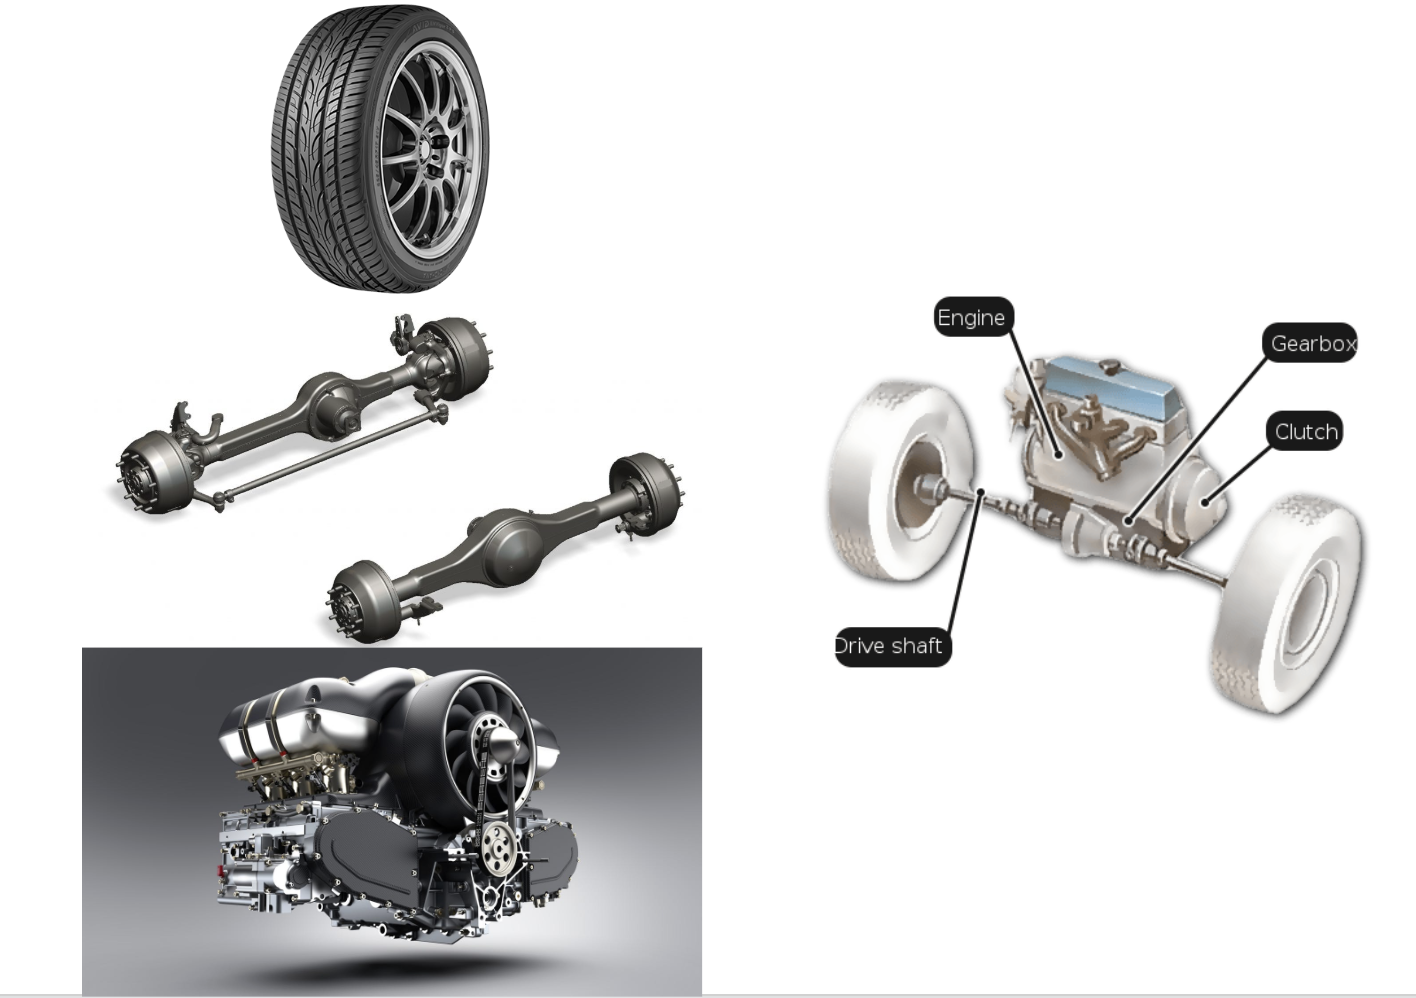
\includegraphics[width=0.5\textwidth]{images/car_example}
	\caption{Tires, engine, and axle can be combined to make the core axle-tire-engine unit of a car.}
\end{figure}

There are different ways to design each of these. They can each be made from a number of materials, and there are different sizes and varieties of each (e.g. 4 vs 6 cylinder engine, snow vs all-season tires, etc.). Furthermore, any \textit{combination} of these different varieties can be put together: we can change the type of tires we have without thinking about what type of axle or motor is in the car. 

\begin{figure}
	\centering
	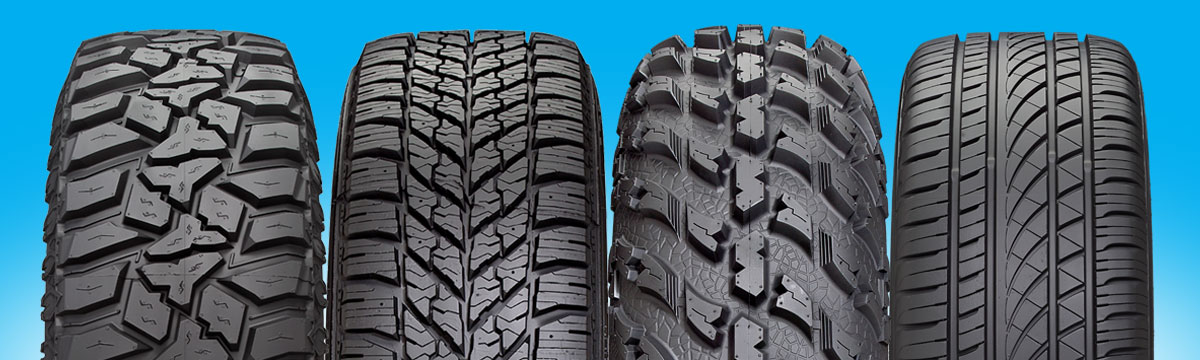
\includegraphics[width=0.5\textwidth]{images/tires.jpg}
	\caption{A variety of tires are available, and each must simply (1) be built to roll and (2) be connectable to an axle}
\end{figure}

We will now look at the benefits of this modularity in car design:

\begin{itemize}
\item \textbf{Teamwork}: Car companies can divide the work amongst multiple
  teams, and those teams won't interfere with each other as they work. One team
  can spend months developing the axle: finding the right alloy, shape, and
  weight to handle the load from the car. Another team can spend months
  developing the engine: trying out different arrangements of the cylinders or
  different numbers of cylinders. What's more, car manufacturers almost always
  outsource the production of their tires to tire manufacturers: they leave the
  decisions on the type of rubber and treads to a team totally outside of their
  company. The modularity of the car allows these teams to work totally
  separately, with the only communication between them the above list: the tire
  must roll and attach to an axle; the engine must spin the axle; and the axle
  must connect to the engine and the tires. Once the teams agree on the way they
  will bolt the systems together, they no longer have to communicate.
    
\item \textbf{Updateability}: Modularity allows car enthusiasts to upgrade and
  customize their vehicles without having to redesign the whole thing. If a
  vehicle owner wants to replace their V6 with a V8, they can do that as long as
  the connections between the motor and the rest of the vehicle are the same
  (i.e. the connection to the axle, to the fuel source, etc). If a vehicle owner
  wants to replace their all season tires for snow tires in the winter, they can
  do that as long as the connection with the rest of the vehicle is the same
  (i.e. the connection to the axle is the same).
\end{itemize}

\subsection{APIs}
\begin{definition}
An \emph{Application Programming Interface}, or API, is a contract between components in a system, expressing what each component can expect from the others. 
\end{definition}

Building on the previous section's example of a vehicle, we can consider the API between the engine manufacturer and the vehicle manufacturer. 

The engine manufacturer can expect the vehicle to:
\begin{itemize}
	\item Have an axle.
	\item Have a fuel source.
	\item Have a cooling source.
	\item Have a control system.
\end{itemize}

The vehicle manufacturer can expect the engine to:
\begin{itemize}
	\item Attach to an axle.
	\item Spin at a given revolution speed.
\end{itemize}

As we saw in the previous section, this type of contract allows division of labor between different teams working on a project to ensure that they can work independently.

Another API exists between a driver and the manufacturer: the driver can expect the car to have a:
\begin{itemize}
	\item Device to turn on/off the car.
	\item Device to steer the car.
	\item Device to accelerate the car.
	\item Device to decelerate the car.
\end{itemize}

The car maker can expect the driver to have
\begin{itemize}
	\item Arms and hands that can turn and push.
	\item Feet and legs that can press.
\end{itemize}

\begin{example}
An API between an ATM and a user. 
\end{example}

From the perspective of a user, an ATM's purpose is to take in a credit card and a specified dollar amount from a user, and output the requested amount of money. The user can expect an ATM to:
\begin{itemize}
	\item Read their credit card.
	\item Specify the card's PIN number.
	\item Specify a requested dollar amount.
	\item Output money and notify their bank of the transaction.
\end{itemize}

An ATM can expect the user to:
\begin{itemize}
	\item Have a credit card.
	\item Type with their fingers.
	\item Read and respond to prompts on the screen.
\end{itemize}

Note that a problem with the API translates to a problem with the end-product. This API doesn't guarantee that a blind person will be able to use the ATM, for example (they won't be able to read). 

\begin{example}
The API between an ATM and a bank.
\end{example}

From the perspective of a bank, an ATM's purpose is to send in credit card info and the requested dollar amount, and fulfill a user request for money only if the bank authenticates the request. 

The bank can expect an ATM to
\begin{itemize}
	\item Accurately send the bank credit card info and a PIN.
	\item Accurately send the bank the requested dollar amount.
	\item Complete the user's transaction only if the bank sends back a confirmation.
\end{itemize}

The ATM can expect the bank to
\begin{itemize}
	\item Receive credit card info and a PIN.
	\item Send back a confirmation or denial.
\end{itemize}

\section{User-oriented Design}

\subsection{Waterfall vs Iterative Design}

\begin{example}
build the highest tower possible in 6 minutes using the following ingredients:\footnote{Adapted from https://tinkerlab.com/spaghetti-tower-marshmallow-challenge/}
\begin{itemize}
	\item 10 sticks of dry spaghetti
	\item One foot of string
	\item One foot of tape
\end{itemize}
\end{example}

This activity generally demonstrates that iteration trumps pre-planning. It's faster to just try out imperfect designs than to try to wait for a perfect idea. With a 6 minute time limit, iteration tends to work out better than pre-planning. 

\begin{definition}
\emph{Waterfall design} is a development process in which each stage of development is finished before the next is started. 
\end{definition}

\afm{I'm unsure about putting this here, shouldn't it just go in a bibliography?}The components of waterfall design \footnote{adapted from https://airbrake.io/blog/sdlc/waterfall-model} are the following:
\begin{enumerate}
	\item Requirements: define what the application should do (essentially, write the API between a user and your product).
	\item Design: decide what the product will look like based on the requirements, and how it will be implemented.
	\item Implementation: build the product based on the design.
	\item Test: ensure the product works as expected.
	\item Deployment: release the product to the users.
\end{enumerate}

\begin{figure}
	\centering
	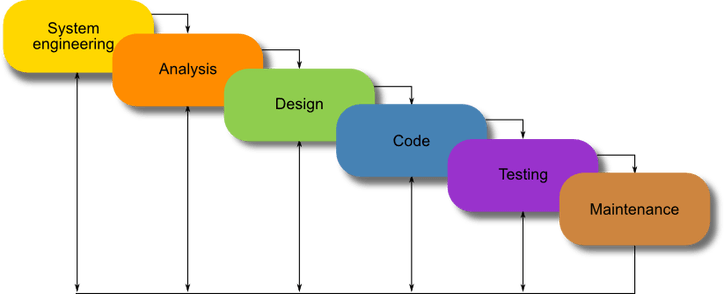
\includegraphics[width=0.5\textwidth]{images/waterfall.png}
	\caption{Waterfall design.}
\end{figure}

In waterfall design, mistakes early in the process can grow fatal. You might spend a lot of time and money going through the full waterfall and developing a final product and then realize that the requirements were wrong. Going back to a previous example, suppose you had designed an ATM thinking that users would be able to read and later found out that blind users must also be able to access the ATM. You would have to completely redesign the system, perhaps having to put speakers into the ATM so that the prompts can be read aloud to the user. 

\begin{definition}
In \emph{iterative design}, many iterations of a project are built and presented to users with the expectation that the requirements and design may need to be adjusted in further iterations. 
\end{definition}

Iterative design entails going through the same 4 steps of specifying requirements, drafting a design, implementing, then deploying. However, less time and money is invested into trying to make the first iteration perfect. The first iteration of a project might look horrible, but users will be able to tell you the fundamental flaws (such as missing requirements) before you start implementing a perfect product for the wrong problem. 

Iterative design is also used in drawing. As shown in \autoref{fig:owl}, professional artists start with a rough sketch of an object before starting to fill in details. The first iteration (top) doesn't look very good, but you might find out that you're missing basic requirements: you might be missing certain body parts, or decide you'd like to add a background or another object. By the second iteration, things look a little better, but you still might find more fundamental errors along the way. By the time you're ready to fill in all of the details in the bottom step, you're confident you're drawing the figure you want to draw. 

\begin{figure}
	\centering
	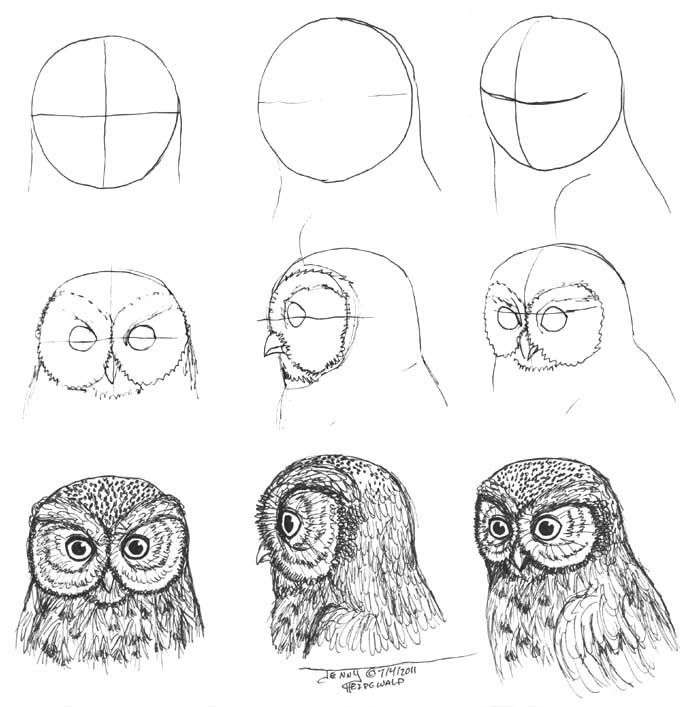
\includegraphics[width=0.5\textwidth]{images/owl.jpg}
	\caption{Iterative drawing of an owl\footnote{Courtesy of https://www.pinterest.com/pin/469289223655955022/}.}
	\label{fig:owl}
\end{figure}

\section{Testing}
Code rarely works the way we would like it to the first time around. 

\begin{definition}
A \emph{software bug}, is an error in a computer program which causes an incorrect or unexpected result, or to behave in unintended way (Wikipedia). 
\end{definition} 

Medium estimated that in 2016 approximately a trillion dollars was lost to the US economy due to software bugs. As one tangible example of the cost of bugs, in 1962 NASA's 18 million dollar Mariner 1 had to be self-destructed mid-flight because of a missing hyphen in the control code.\footnote{https://medium.com/@ryancohane/financial-cost-of-software-bugs-51b4d193f107}

For this reason, developers are always expected to carefully test the code they write to ensure there are no bugs. In addition, even relatively small software firms often have an entire team whose sole job is to test code written by the developers. Their job is to use the product in a variety of potentially unexpected ways. In essence, they try their best to break the code. The product is not ready for the market until the testing team is unable to break it, and all of its behaviors are as expected by the API for the product. 

	\pagebreak

\appendix
\addappheadtotoc
\appendixpage
	\section*{Possible appendices topics}

\begin{itemize}

	\item Comparing floating point numbers.
	\item Type conversion.
	\item Useful math functions, e.g. \ic{min()}, \ic{log}.

\end{itemize}

\section{Java Reserved Words}

TODO: fill this in

\end{document}
